\documentclass{article}[12pt]
\usepackage{fancyhdr, fancybox, tabularx, verbatim, epsfig}
%\usepackage{fancyhdr, graphicx, fancybox, wrapfig, epic, ecltree, tabularx,
%  verbatim, alltt, ifthen, boxedminipage, epsfig}

\includeonly{overview, high_level, data_formats, data_interface, examples,
  advanced, functions, matrix_free}

%\setlength{\oddsidemargin}{0.4\oddsidemargin}
%\setlength{\evensidemargin}{0.4\evensidemargin}
%\setlength{\topmargin}{0.0\topmargin}
%\setlength{\textheight}{1.16\textheight}
%\setlength{\textwidth}{1.29\textwidth}
\setlength{\oddsidemargin}{0.3\oddsidemargin}
\setlength{\evensidemargin}{0.3\evensidemargin}
\setlength{\topmargin}{0.0\topmargin}
\setlength{\textheight}{1.16\textheight}
\setlength{\textwidth}{1.39\textwidth}

%
% macros for formatting symbols for reals, integers, etc.
%

\newcommand{\Az}  {{\bf Aztec}}
\newcommand\R     {{\rm \bf R}}
\newcommand\I     {{\rm \bf I}}
\newcommand\C     {{\rm \bf C}}

%
% define boxes for describing variables, etc
%

\def\optionbox#1#2{\noindent$\hphantom{hix}${\parbox[t]{2.10in}{\it
#1}}{\parbox[t]{3.9in}{#2}} \\[1.1em]}

\def\choicebox#1#2{\noindent$\hphantom{hixthere}$\parbox[t]{2.10in}{\sf
#1}\parbox[t]{3.5in}{#2}\\[0.8em]}

\def\structbox#1#2{\noindent$\hphantom{hix}${\parbox[t]{2.10in}{\it
#1}}{\parbox[t]{3.9in}{#2}} \\[.02cm]}

\def\in{\hskip .2in \=}
\def\hsp{\hskip .4in \=}
\def\sp{\hskip .18in \=}
\def\sh{\hskip .18in }
\def\bb{\hskip .034in }
\def\lil{\hskip .1in }


\def\protobox#1{\vspace{2em}{\flushleft{\bf Prototype}
\hrulefill}\flushleft{\fbox{\parbox[t]{6in}{\vspace{1em}{\sf
#1}\vspace{1em}}}}}

%--- redefine this for the tabularx environment

\newcolumntype{Y}{>{\raggedright\arraybackslash}X}
\newcolumntype{Z}{>{\small\raggedright\arraybackslash}X}

%
% ***********************************************************************
% * 02 July 1993: McCorkle                                              *
% * Define a macro that will lightly print the word `DRAFT' diagonally  *
% * across each page of the document. This macro was obtained from the  *
% * NMSU math department                                                *
% *                                                                     *
% * Usage: \draft                                                       *
% ***********************************************************************
%
\def\draft{%
\special{!userdict begin /bop-hook{gsave
200 30 translate 65 rotate
/Times-Roman findfont 216 scalefont setfont
0 0 moveto 0.9 setgray (DRAFT) show grestore}def end}
}

\renewcommand\baselinestretch{0.9}

\begin{document}

\large
\pagenumbering{roman}

%\draft                                   % Lightly print `DRAFT' on every
                                         % page of the document

%
% Stuff for SAND report style from B.A. Hendrickson, SNL, 1422
%
\hspace{2.22in}
SAND99--8801J
\hfill
Distribution

\hspace{2.07in}
Unlimited Release
\hfill
Category UC--405
\begin{center}
Printed Nov 1999
\end{center}

\vspace{0.8in}

\begin{center}
%{\Large{\bf \Az{} User's Guide$^\ast$ \\ Version 2.1}}
  {\Large{\bf Official \Az{} User's Guide\footnote{This work was supported by 
	the
        Applied Mathematical Sciences program, U.S. Department of Energy,
        Office of Energy Research, and was performed at Sandia National
        Laboratories, operated for the U.S. Department of Energy under contract
        No. DE-AC04-94AL85000. The \Az{} software package was developed by the
        authors at Sandia National Laboratories and is under copyright
        protection} \\ Version 2.1}}

\vspace*{0.4in}

Ray S. Tuminaro\footnote{Applied \& Numerical Mathematics Department;
  tuminaro@cs.sandia.gov; (925) 294-2564}
\,\,\,\,Mike Heroux\footnote{Applied \& Numerical Mathematics Department;
  maherou@cs.sandia.gov; (320) 845-7695}
\,\,\,\,Scott A. Hutchinson\footnote{Parallel Computational Sciences Department;
  sahutch@cs.sandia.gov; (505) 845-7996}
\,\,\,\, John N. Shadid\footnote{Parallel Computational Sciences Department;
  jnshadi@cs.sandia.gov; (505) 845-7876}
\\

Massively Parallel Computing Research Laboratory \\
Sandia National Laboratories \\
Albuquerque, NM \, 87185

\vspace*{.9in}

\end{center}

{\centering\large Abstract \\[1em]}

\Az{} is an iterative library that greatly simplifies the parallelization
process when solving the linear systems of equations $Ax = b$ where $A$ is a
user supplied $n \times n$ sparse matrix, $b$ is a user supplied vector of
length $n$ and $x$ is a vector of length $n$ to be computed. \Az{} is intended
as a software tool for users who want to avoid cumbersome parallel programming
details but who have large sparse linear systems which require an efficiently
utilized parallel processing system.  A collection of data transformation tools
are provided that allow for easy creation of distributed sparse unstructured
matrices for parallel solution. Once the distributed matrix is created,
computation can be performed on any of the parallel machines running \Az{}:
workstation clusters (DEC, SGI, SUN, LINUX, etc.), Cray T3E,
Intel TeraFlop, Intel Paragon, IBM SP2, nCUBE 2
as well as other
MPI platforms, vector machines or serial machines.

\Az{} includes a number of Krylov iterative methods such as conjugate gradient
(CG), generalized minimum residual (GMRES) and stabilized biconjugate gradient
(BiCGSTAB) to solve systems of equations.  These Krylov methods are used in
conjunction with various preconditioners such as polynomial or domain
decomposition methods using LU or incomplete LU factorizations within
subdomains. Although the matrix $A$ can be general, the package has been
designed for matrices arising from the approximation of partial differential
equations (PDEs).


\vfill

\newpage

%--- heading stuff

\pagestyle{fancyplain}
\addtolength{\headwidth}{\marginparsep}
%\addtolength{\headwidth}{\marginparwidth}
%--- remember section title
\renewcommand{\sectionmark}[1]{\markboth{#1}{}}
%\renewcommand{\subsectionmark}[1]{\markright{\thesubsection\ #1}}
%\lhead[\fancyplain{}{\bfseries\thepage}]%
%      {\fancyplain{}{\bfseries\rightmark}}
\rhead[\fancyplain{}{\bfseries\leftmark}]%
      {\fancyplain{}{\bfseries\thepage}}
\cfoot{}
%\rfoot{\leftmark\\\rightmark}

\large
\tableofcontents

\newpage

{\flushleft {\bf Notation Conventions} \hrulefill
\\[0.5em]

Different fonts are used to indicate program fragments, keys words, variables,
or parameters in order to clarify the presentation.  The table below describes
the meaning denoted by these different fonts.\\[3em]

\begin{tabularx}{\textwidth}{lX} \hline \\
{\bf Convention} & {\bf Meaning} \\[1.25em]

\tt typewriter & File names, code examples and code
fragments. \\

{\sf sans serif} & C language elements such as function names and constants
when they appear embedded in text or in function definition syntax
lines. \\

{\it italics\/} & Parameter and variable names when they appear embedded in
text or function definition syntax lines. \\

{\bf AZ\_ } & C language elements such as function names and constants which
are supplied by the \Az{} library. \\[1em] \hline
\end{tabularx}
%
\vskip 3.0em
\flushleft {\bf Code Distribution} \hrulefill
\\[0.5em]

\Az{} is publicly available for research purposes and may be licensed for
commercial application.  The code is distributed along with technical
documentation, example C and Fortran driver routines and sample input files via
the internet.  It may be obtained by contacting one of the authors listed on
page i of this report or from the \Az{} web site at
\tt http://www.cs.sandia.gov/CRF/aztec1.html.}

\newpage
\pagenumbering{arabic}

% @HEADER
% ***********************************************************************
% 
%            Trilinos: An Object-Oriented Solver Framework
%                 Copyright (2001) Sandia Corporation
% 
% Under terms of Contract DE-AC04-94AL85000, there is a non-exclusive
% license for use of this work by or on behalf of the U.S. Government.
% 
% This library is free software; you can redistribute it and/or modify
% it under the terms of the GNU Lesser General Public License as
% published by the Free Software Foundation; either version 2.1 of the
% License, or (at your option) any later version.
%  
% This library is distributed in the hope that it will be useful, but
% WITHOUT ANY WARRANTY; without even the implied warranty of
% MERCHANTABILITY or FITNESS FOR A PARTICULAR PURPOSE.  See the GNU
% Lesser General Public License for more details.
%  
% You should have received a copy of the GNU Lesser General Public
% License along with this library; if not, write to the Free Software
% Foundation, Inc., 59 Temple Place, Suite 330, Boston, MA 02111-1307
% USA
% Questions? Contact Michael A. Heroux (maherou@sandia.gov) 
% 
% ***********************************************************************
% @HEADER

\documentclass[10pt,relax]{SANDreport}
\usepackage{amsmath,amsthm}
\usepackage{amssymb}
\usepackage{amsfonts}
\usepackage{palatino}
\usepackage{rotating,tabularx}

\def\choicebox#1#2{\noindent$\hphantom{th}$\parbox[t]{1.8in}{\sf
#1}\parbox[t]{4.5in}{#2}\\[0.8em]}

\author{Marzio Sala, Michael A. Heroux\\
Computational Mathematics and Algorithms Department \\ [10pt]
William F. Spotz, Eric T. Phipps \\
Applied Computational Methods Department \\ [10pt]
Sandia National Laboratories \\
P.O. Box 5800 \\
Albuquerque, NM 87185-1110 \\
}

\title{An Overview of PyTrilinos}
\SANDnum{SAND2005-XXXX}
\SANDauthor{
Marzio Sala, William F. Spotz, Eric T. Phipps, Micheal A. Heroux}

\SANDprintDate{June 2005}
\SANDreleaseType{Unlimited Release}

\newcommand{\PyTrilinos}{{PyTrilinos}}
\newcommand{\Trilinos}{{Trilinos}}
\newcommand{\TrilinosTM}{Trilinos \copyright}
\newcommand{\trilinos}{{Trilinos}}
\newcommand{\ifpack}{{Ifpack}}
\newcommand{\aztecoo}{{AztecOO}}
\newcommand{\amesos}{{Amesos}}
\newcommand{\epetra}{{Epetra}}
\newcommand{\ml}{{ML}}
\newcommand{\mb}[1]{{\mathbf {#1} }}
\newcommand{\teuchos}{{Teuchos}}
\newcommand{\triutils}{{Triutils}}
\newcommand{\metis}{{METIS}}

\newcommand{\ie}{i.e., }
\newtheorem{assumption}{Assumption}[section]
\newtheorem{lemma}{Lemma}[section]
\newtheorem{proposition}{Proposition}[section]
\newtheorem{corollary}{Corollary}[section]
\newtheorem{theorem}{Theorem}[section]
\newtheorem{algorithm}{Algorithm}[section]
\newtheorem{definition}{Definition}[section]
\newtheorem{property}{Property}[section]
\newtheorem{interface}{Interface}[section]
\newtheorem{remark}{Remark}
\newcommand{\note}[1]{\begin{center}\fbox{\bf #1}\end{center}}


\def\choicebox#1#2{\noindent$\hphantom{th}$\parbox[t]{3.0in}{\sf
#1}\parbox[t]{3.35in}{#2}\\[0.8em]}

\begin{document}

\maketitle

\begin{abstract}
\PyTrilinos\ is a collection of Python modules that are useful for
serial and parallel scientific computing. This collection contains
modules that cover serial dense linear algebra, parallel sparse linear
algebra, direct and iterative linear solution techniques, domain
decomposition and multilevel preconditioners, nonlinear solvers and
continuation algorithms. Also included are a variety of related
utility functions and classes, including distributed I/O and matrix generation
utilities.
\PyTrilinos\ vector objects are integrated with the popular Numeric
Python module, gathering together a variety of high-level distributed
computing with serial vector operations.

PyTrilinos is defined as a set of interfaces to already available non-Python
libraries.
This hybrid framework uses Python as front-end, and
efficient precompiled libraries for all computationally expensive tasks. Thus,
we take advantage of both the flexibility and ease of use of Python,
and the efficiency of the underlying C++, C and FORTRAN numerical
kernels. The presented numerical results show that, if properly used, the
overhead required by the Python interpreter is negligible. The presented
numerical results show that, if properly used, the overhead required by the
Python interpreter is negligible.

To run in parallel, \PyTrilinos\ simply requires a standard Python
interpreter.  The fundamental MPI calls are abstracted beneath the
Epetra module layer, and all inter-processor communications by all
\PyTrilinos\ modules are handled using Epetra communicators. This
makes serial and parallel scripts using \PyTrilinos\ virtually
identical.
\end{abstract}

\clearpage
\section*{Acknowledgments}
The authors would like to acknowledge the support of the ASCI and LDRD
programs that funded development of Trilinos, and all the Trilinos
developers for their contribution to Trilinos, without which
\PyTrilinos\ would not exist.

\medskip

\SANDmain
\tableofcontents
\newpage

%-----------------------------------------------------------------------------
\section{Introduction}
\label{sec:intro}
%-----------------------------------------------------------------------------

The choice of the programming language for the development and usage of
large-scale, high-performance numerical algorithms is often a thorny issue.
Ideally, the programming language is only a tool used to produce a working
library or application. In practice, the are important differences between the
several programming languages made available to developers---from FORTRAN77 or
FORTRAN90, to C and C++, Java, Python, MATLAB, and several others. An important
distinction can be made between {\sl interpreted} languages and {\sl compiled}
languages. For the former, the list of instructions (called {\sl script}) is
translated at run-time by an interpreter, then executed; for the latter, the
code is compiled and an executable is created. It is well known that
interpreted code is easier to use and debug as the interpreter will analyze each
instruction as it is executed. This comes at a computational price, since the interpreter
may require several CPU cycles to parse each instruction. Therefore,
interpreted languages are usually disregarded by developers of
high-performance applications (often as a pre-conceptual idea). Almost all
high-performance libraries are written in compiled languages
such as C, C++ or FORTRAN. Using these languages, developers can obtain 
high performance and portable codes,
since these languages are reasonably well standarized and compilers quite
mature on almost all platforms.  However,
these languages require constant attention to low-level system
programming, like memory allocation and deallocation.  Because
compilation and linking are essential steps, the development cycle can
be slowed down considerably, sometimes making the development of new algorithm
problematic.

As developers of numerical algorithms,
our interest is in a high-level, flexible programming environment,
with performance comparable to that of native C, C++ or FORTRAN
code. Flexibility is fundamental to allow rapid prototyping, in the
sense that the developer should be able to write a basic code
satisfying his or her needs in a very short time.  However, it is
almost impossible for a single programming language to be at the same
time easy-to-use, allow fast development, and produce optimized
executables. Indeed, the goals of efficiency and flexibility are often
in conflict with each other.
From our point of view, the key observation is that, for most
applications, the time-critical portion of the code that requires the
efficiency of a compiled language is related to a small set of
self-contained functions or classes. Therefore, one can adopt an
interpreted (and possibly interactive) language, without a big
performance degradation, provided there is a robust interface between
the interpreted and compiled languages. Among the available scripting
languages, we decided to adopt Python 
(see, for instance, \cite{python-book}).  Python
is an interpreted, interactive, object-oriented programming
language, which combines remarkable power with very clean syntax (it
is often observed that well-written Python code reads like pseudo
code).  Perhaps most importantly, it can be easily extended using
modules written in C or C++ for all performance critical tasks.

This article describes a collection of numerical analysis algorithms, called
PyTrilinos, 
built on top of the Trilinos
project~\cite{Trilinos-home-page,Heroux:2005:OTP}.  It adds significant power
to the interactive Python session by exposing the user to high-level commands
and classes for the creation, handling and usage of serial dense and
distributed sparse linear algebra objects. Using \PyTrilinos, an interactive
Python session becomes a powerful data-processing and system-prototyping
environment that can be used to test, validate, use
and extend serial and parallel numerical algorithms.
In our opinion, Python naturally complements
system languages like C, C++ and FORTRAN rather than competing with
them. Equivalently, PyTrilinos complements Trilinos by offering a rapid
development cycle for some of its capabilities.

%Python is a high-level general purpose programming language. Because
%code is automatically compiled to byte code and executed, Python is
%suitable for use as a scripting language.  In typical Python
%development, a system's frontend and infrastacture may be written in
%Python for ease of development and modification, but the kernel is
%still written in C or C++ for efficiency.  We use Python as a glue
%between different modules, written in high-performance languages; each
%of these modules is an already available library, dynamically loaded
%by Python when required.  

\smallskip

This document is organized as follows. Section~\ref{sec:design} describes the
project design, the organization of PyTrilinos and its division into modules.
Comments on the usage of
parallel, MPI Python scripts using PyTrilinos are reported in
Section~\ref{sec:serial}. 
Section~\ref{sec:related} positions PyTrilinos with respect to similar
projects. 
Examples of usage and comparisons between Trilinos
and PyTrilinos codes are reported in Section~\ref{sec:comparision}.
Concluding remarks are reported in Section~\ref{sec:concluding}.

%-----------------------------------------------------------------------------
\section{Project Design}
\label{sec:design}
%-----------------------------------------------------------------------------

%-----------------------------------------------------------------------------
\subsection{Why Python}
\label{sec:why}
%-----------------------------------------------------------------------------

Python has emerged as an excellent choice for scientific computing
because of its simple syntax, ease of use, and elegant
multi-dimensional array arithmetic. Its interpreted evaluation allows
it to serve as both the development language and the command line
environment in which to explore data. Python also excels as a ``glue''
language between a large and diverse collection of software packages
-- a common need in the scientific arena.

Python combines remarkable power with very clean syntax. It has
modules, classes, exceptions, high-level dynamic data types, automatic
memory management that frees the user from most hassles of memory
allocation, and much more. Python also has some features that make it
possible to write large programs, even though it lacks most forms of
compile-time checking: a program can be constructed out of modules,
each of which defines its own namespace. Exception handling makes it
possible to catch errors where required without cluttering the code
with error checking.

Python's development cycle is dramatically shorter than that of
traditional tools. In Python, there are no compile or link
steps--Python programs simply import modules at runtime and use the
objects they contain. Because of this, Python programs run immediately
after changes are made. Python integration tools make it usable in
hybrid, multi-compont applications. As one consequence, systems can
simultaneously utilize the strengths of Python for rapid development,
and of traditional languages such as C for rapid execution.  This
flexibility of development modes is crucial in realistic environments.

\note{Why no other scripting languages?}

%-----------------------------------------------------------------------------
\subsection{Multilevel Organization of PyTrilinos}
\label{sec:multilevel}
%-----------------------------------------------------------------------------
  
\PyTrilinos\ is a designed as a modular multilevel framework, and it
takes advantage of several programming languages at different levels.
The key components are:
\begin{enumerate}

\item {\bf Trilinos}, a set of numerical solver packages in active
  development that allows high-performance scalable linear algebra
  operations for problems defined on sparse matrices. Trilinos
  contains more that half a million of code lines, and it can
  interface to several third-party libraries. The source codes of the
  ``stable'' linear algebra packages of Trilinos account for about 300,000
  code lines, divided in about 67,000 code lines for distributed linear
  algebra objects and utilities, 20,000 code lines for direct solvers and
  interfaces to third-party direct solvers, 128,000 code lines for multilevel
  preconditioners, and 76,000 code lines for other algebraic preconditioners
  and Krylov accelerators.

\item {\bf Numeric}, a well-established Python module to handle
  matrices and vectors; see~\cite{numeric}.

\item {\bf SWIG}, the Simplified Wrapper and Interface Generator,
  which is a preprocessor that turns ANSI C/C++ declarations into
  scripting language interfaces, and produces a fully working Python
  extension module; see~\cite{swig}.

\item {\bf Distutils}, a Python module with utilities aimed at the
  portable distribution of both pure Python modules and compiled
  extension modules.  Distutils has been a part of the standard Python
  distribution since Python version 2.2.

\end{enumerate}

A description of the organization of  the linear algebra modules of
PyTrilinos, with some of the third-party libraries can be accessed,
is reported in Figure~\ref{fig:organization}.

\begin{figure}
\begin{center}
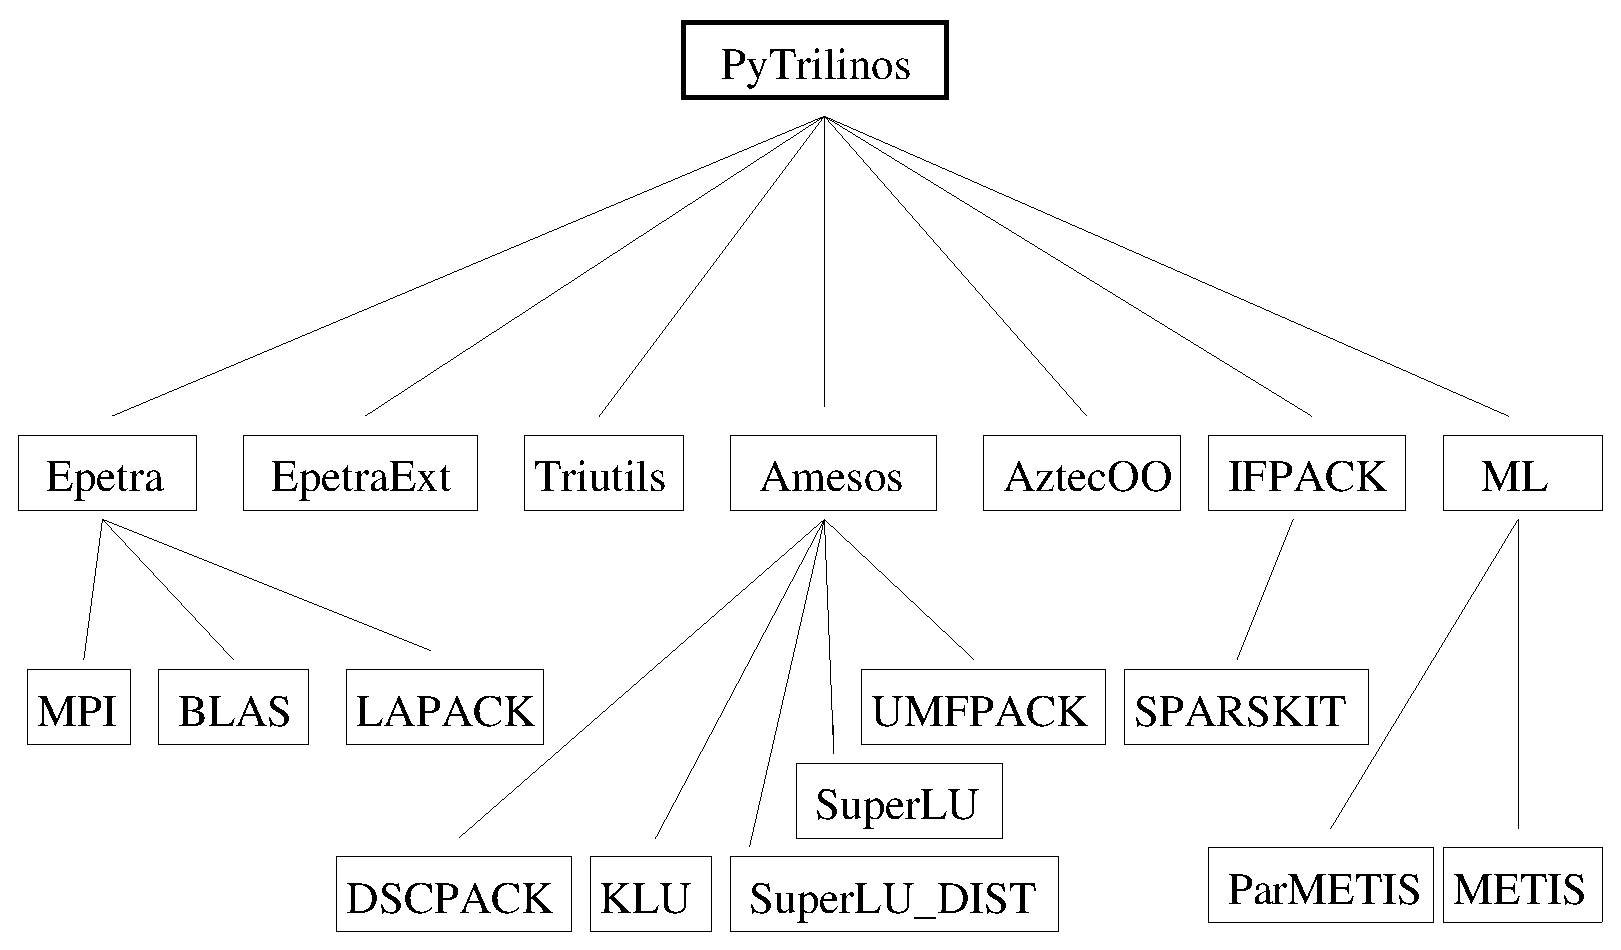
\includegraphics[width=12cm]{../UsersGuide/organization.eps}
\caption{Organization of the linear algebra modules of PyTrilinos.}
\label{fig:organization}
\end{center}
\end{figure}

%-----------------------------------------------------------------------------
\subsection{PyTrilinos Organization}
\label{sec:organization}
%-----------------------------------------------------------------------------

\PyTrilinos\ reflects the Trilinos organization by presenting a series
of {\sl modules}, each of them wraps a given Trilinos {\sl package},
 where a package is an integral unit usually
developed by a small team of experts in a particular area.
Trilinos packages that support namespaces have a Python submodule for
each namespace.  Algorithmic capabilities are defined within
independent packages. At present, the modules of \PyTrilinos\ are:

\begin{enumerate}

\item {\bf Epetra}, a collection of concrete classes to support the
construction and use of vectors, sparse distributed graphs, and dense and
distributed sparse matrices. It provides serial, parallel and distributed
memory capabilities. Epetra supports double-precision floating point data only
(no single-precision or complex), and uses BLAS and LAPACK where possible, and
as a result has good performance characteristics.  See~\cite{epetra-guide} for
more details. 
\item {\bf EpetraExt} offers a variety of extension capabilities to
  the Epetra package, such as input/output and coloring algorithms.
  The I/O capabilities make it possible to read and write generic
  Epetra objects (like maps, matrices and vectors).

\item {\bf Triutils} allows the creation of several matrices, like the
  MATLAB's {\tt gallery} function, and it can be useful for examples
  and testing. Some input capabilities make it possible to read a matrix in
  Harwell/Boeing or MatrixMarket format, therefore accessing a large variety
  of well-recognized test cases for dense and sparse linear algebra.

\item {\bf Amesos} contains a set of clear and consistent interfaces
  to the following third-party serial and parallel sparse direct
  solvers: UMFPACK~\cite{umfpack-acm-toms},
  PARDISO~\cite{pardiso-manual}, TAUCS~\cite{taucs-home-page}, SuperLU
  and SuperLU\_DIST~\cite{superlu-manual},
  DSCPACK~\cite{dscpack-manual}, MUMPS~\cite{mumps-manual}, and
  ScaLAPACK~\cite{scalapack-book,scalapack}. As
  such, \PyTrilinos\ makes it possible to access state-of-the-art
  direct solver algorithms developed by groups of specialists, and
  written in different languages (C, FORTRAN77, FORTRAN90), in both
  serial and parallel environments. By using Amesos, more than 350,000 code lines (without
  considering BLAS, LAPACK, and ScaLAPACK) can be easily accessed from any
  code based on Trilinos (and therefore PyTrilinos).  We refer to the Amesos
  reference guide~\cite{Amesos-Reference-Guide} for more details.

\item {\bf AztecOO} contains preconditioned Krylov accelerators, like
  CG, GMRES and several others~\cite{golub96matrix}, based on the popular Aztec
  library~\cite{aztecoo-guide}.  One-level domain decomposition
  preconditioners based on incomplete factorizations are available.

\item {\bf IFPACK} contains object-oriented algebraic preconditioners,
  compatible with Epetra and AztecOO.  It supports construction and
  use of parallel distributed memory preconditioners such as
  overlapping Schwarz domain decomposition with several local solvers.
  IFPACK can take advantage of SPARSKIT~\cite{sparskit}, a venerable
  but successful software package; see~\cite{ifpack-guide}.

\item {\bf ML} contains a set of multilevel preconditioners based on
  aggregation procedures for serial and vector problems compatible with Epetra
  and AztecOO. ML can take
  advantage of the METIS~\cite{metis} ParMETIS~\cite{parmetis}
  libraries to create the aggregates.  For a general introduction to
  ML and its applications, we refer to the ML Users
  Guide~\cite{ml-guide}.

\end{enumerate}

Note that all third-party libraries (except BLAS and LAPACK) are
optional and do not need to be installed to use \PyTrilinos\ (or
Trilinos). 

All the presented modules depend on Epetra, since Epetra is the ``language''
of Trilinos, and offers a convenient set of interfaces to define distributed
linear algebra objects.  \PyTrilinos\ cannot be used without the Epetra
module, while all the other modules can be enabled or disabled in the
configuration phase of Trilinos.

%-----------------------------------------------------------------------------
\section{Serial and Parallel Environments}
\label{sec:serial}
%-----------------------------------------------------------------------------

Although testing and development of high-performance algorithms can be done in
serial environments, parallel environments still constitute the most
important field of application for most of Trilinos' algorithms. However,
  Python itself does not provide any parallel support. Because of this reason,
  several projects entered the scene, to fulfill the gap between Python and
  MPI applications. We have analyzed the following:
\begin{itemize}
\item {\bf MPI Python (pyMPI)} is a framework for developing parallel Python
  applications using MPI~\cite{MPI-Python};
\item {\bf PyPAR} is a more light-weight wrapper of the MPI library
  for Python~\cite{pypar}.
\item {\bf Python BSP} supports the more high-level Bulk Synchronous
  Parallel approach~\cite{bsp}
\end{itemize}

All these projects allow the use of Python through the interactive  prompt, 
  but an additional overhead is introduced. Besides, none of these projects
  defines a well-recognized standard, since they are still under heavy
  development. 

Our approach is somehow complementary to the efforts of these projects. 
We decided to use a standard, out-of-the-box, Python interpreter, then wrap 
only the very basic MPI functions 
(MPI\_Init(), MPI\_Finalize(), and MPI\_COMM\_WORLD). By wrapping these three
objects, one can define an MPI-based Epetra communicator, on which
all wrapped Trilinos packages are already
based. This reflects the philosophy of all the
considered
Trilinos packages, that have no explicit dependency on MPI communicators, and
accept the pure virtual class Epetra\_Comm instead. PyTrilinos scripts create
a communicator using command
\begin{verbatim}
    >>> comm = Epetra.PyComm()
\end{verbatim}
which returns an Epetra.SerialComm if \PyTrilinos\ has been compiled
in serial mode, or an Epetra.MpiComm if \PyTrilinos\ has support for
MPI. By using Epetra.PyComm, \PyTrilinos\ scripts are virtually
identical for both serial and parallel runs, and generally reads:
\begin{verbatim}
    >>> from PyTrilios import Epetra
    >>> Epetra.Init()
    >>> comm = Epetra.PyComm()
        ...
    >>> Epetra.Finalize()
\end{verbatim}
A pictorial representation of how communication are handled in
the case of two  processors is given in Figure~\ref{fig:distributed}. For
serial runs, both Init() and Finalize() are empty instructions.

\smallskip

The major disadvantage of this approach is that Python cannot be run
interactively if more than one processor is used, and we experienced problems
with some MPI interpreters (in particular MPICH) to execute Python scripts.
Besides, although all the most important MPI calls are available through
Epetra.Comm objects (for example, the rank of a process is returned by method
                     {\tt Comm.MyPID()} and the number of processes involed in
                     the computation by method {\tt Comm.NumProc()}), not all
the functions specified by the MPI forum are readily available through the
Comm object.  For example, there are no point-to-point communications, or
non-blocking functions. Also, PyTrilinos always uses MPI\_COMM\_WORLD as basic
communicator.

In our opinion, these are only minor drawbacks, and the list
of advantages is much longer. 
First, since all
calls are handled by Epetra, no major overhead occurs, other than that of
parsing a Python instruction. Second, all PyTrilinos modules that require
direct MPI calls can dynamic cast the Epetra.Comm object, retrive the MPI
communicator object, then use direct C/C++ MPI calls. As such, the entire set of MPI
function is available to developers. Third, a standard Python interpreter is
required. Finally, serial and paralle scripts are identical, and 
 PyTrilinos scripts can be run in parallel
by using an instruction of type
\begin{verbatim}
    % mpirun -np 4 python ./my-script.py
\end{verbatim}
at the shell prompt, where {\tt my-script.py} contains at least the basic
instructions required to define an Epetra.PyComm.

\begin{figure}
\begin{center}
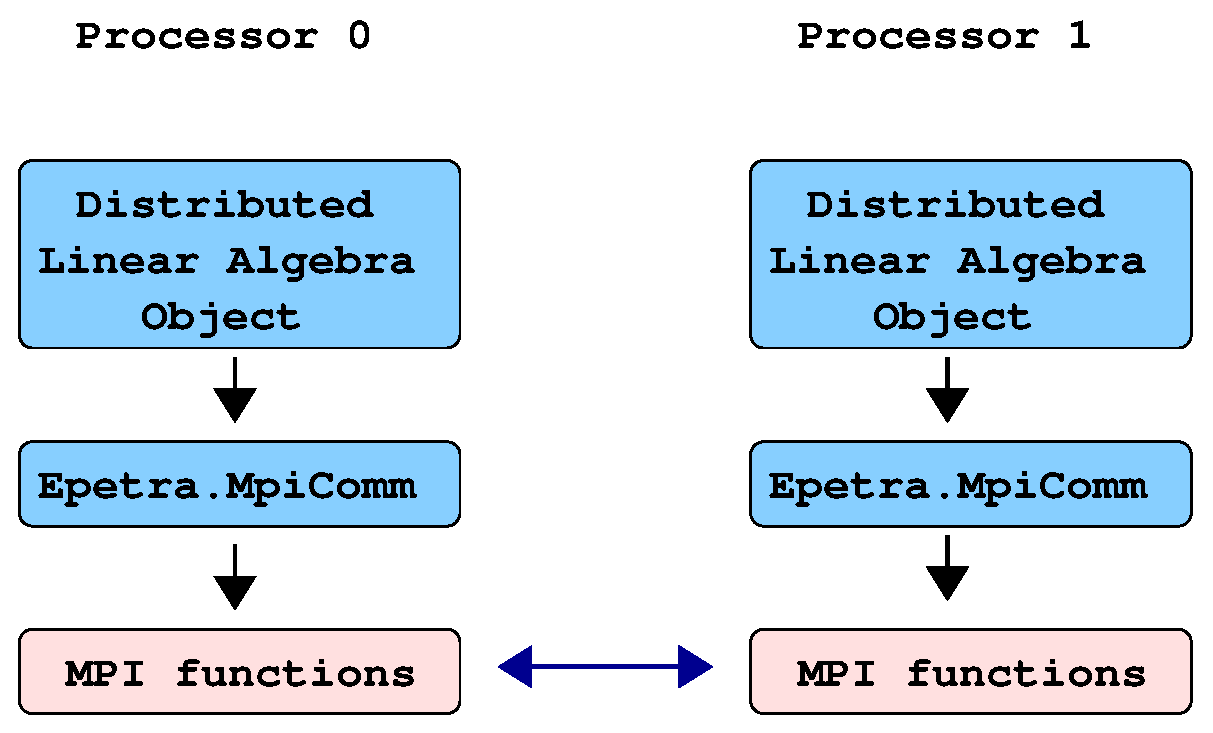
\includegraphics[height=5cm]{../UsersGuide/distributed_object.eps}
\caption{All distributed PyTrilinos objects are based on the Epetra.MpiComm
  object, which takes care of calling MPI functions for intra-processor
    communications.}
\label{fig:distributed}
\end{center}
\end{figure}


%-----------------------------------------------------------------------------
\section{Using PyTrilinos}
\label{sec:using}
%-----------------------------------------------------------------------------

In order to present the functionalities of PyTrilinos, this Section will
briefly describe the main capabilities of all modules, together with a brief
mathematical background of the implemented algorithms.

%-----------------------------------------------------------------------------
\subsection{The Epetra Module}
\label{subsec:epetra}
%-----------------------------------------------------------------------------

Two Epetra objects are important for this
  discussion. The first object is a {\sl communicator}, which
  encapsulates all the inter-processor data exchange. The second
  object is a {\sl map}, which describes the domain decomposition of
  distributed linear algebra objects. Serial runs make use of trivial
  communicators and maps; parallel runs adopt an MPI-based
  communicator and support arbitrary maps.
  
Epetra provides an extensive set of classes to create and fill
distributed sparse matrices. These classes allow row-by-row or
element-by-element constructions. Support is provided for common
matrix operations, including scaling, norm, matrix-vector
multiplication and matrix-multivector multiplication.  Using Epetra
objects, applications do not need to know about the particular storage
format, and other implementation details such as data layout, the
number and location of ghost nodes. Matrices can be stored row-by-row using
class Epetra.CrsMatrix, and vectors with classes Epetra.Vector and
Epetra.MultiVector.
Another useful class is Epetra.FECrsMatrix.  The most important
additional feature provided by the Epetra.FECrsMatrix compared
to Epetra.CrsMatrix, is the capability to set non-local matrix
elements. Serial dense linear algebra is supported 
(as a light-weight on the top of BLAS and LAPACK) through classes
Epetra.SerialDenseVector and Epetra.SerialDenseMatrix.
 Class Epetra.Time can be used
to track the elapsed CPU time, and class Epetra.CrsGraph to define distributed
graphs.

%-----------------------------------------------------------------------------
\subsection{The Triutils Module}
\label{subsec:triutils}
%-----------------------------------------------------------------------------

Triutils provides matrix reading and matrix generation capabilities. This
module is mainly meant for testing solvers. A function is available to read a
matrix from the popular Harwell/Boeing format.
Several matrices, corresponding to finite difference discretization of model
problems, can be generated using the matrix gallery of Triutils, which
provides functionalities similar to that of the MATLAB's {\tt gallery}
command; see~\cite[Chapter 5]{Trilinos-tutorial} for more details.

%-----------------------------------------------------------------------------
\subsection{The Amesos Module}
\label{subsec:amesos}
%-----------------------------------------------------------------------------

Once a (square) sparse matrix and two vectors are created, an
important problem is how to solve the corresponding linear system
\begin{equation}
  \label{eq:lin_sys}
  A X = B
\end{equation}
where $A \in \mathbb{R}^{n \times n}$ is a sparse linear operator, $X
\in \mathbb{R}^{n \times m}$ and $B \in \mathbb{R}^{n \times m}$ are
the solution and right-hand side, respectively. Parameter $n$ is the
global dimension of the problem, and $m$ is the number of vectors in
the multi-vectors $X$ and $B$.  (If $m = 1$, then $X$ and $B$ are
``normal'' vectors.)  Linear systems of type (\ref{eq:lin_sys}) arise
in a variety of applications, and constitute the innermost
computational kernel, and often the most time-consuming of several
numerical algorithms. An efficient solver for Equation
(\ref{eq:lin_sys}) is of fundamental importance for most PDE solvers,
both linear and non-linear.

\smallskip

Probably, the most robust strategy to solve (\ref{eq:lin_sys})
is to factorize the linear matrix $A$ into the product of two matrices
$L$ and $U$, so that $A = L \, U$, and the linear systems with $L$ and
$U$ are readily solvable. Typically, $L$ and $U$ are a lower and upper
triangular matrix, respectively, and the process is referred to as
Gaussian elimination. In PyTrilinos, the direct solution of large linear
system is performed by the Amesos module, which defines interfaces to
third-party direct solvers.
All Amesos objects are constructed from the function class {\tt
  Amesos}.   The main goal of this class is to allow the user to select
any supported (and enabled at configuration time) direct solver,
simply changing an input parameter. An example of script reading the linear
system stored in the Harwell/Boeing format, the solving the problem using
SuperLU is reported in Figure~\ref{fig:amesos}.
Several parameters, specified using Python's dictionaries, are available to toggle the selected Amesos solver.

\begin{figure}
\begin{center}
\begin{tabular}{| p{12cm} |}
\hline
\\
\footnotesize
\begin{minipage}{11.5cm}
\begin{verbatim}
#! /usr/bin/env python
try:
  from PyTrilinos import Amesos, Triutils, Epetra
except ImportError:
  raise ImportError, "error w/ Amesos or Triutils or Epetra"

Epetra.Init()
Comm = Epetra.PyComm()
Map, Matrix, LHS, RHS, Exact = Triutils.ReadHB("fidap035.rua", Comm)

Problem = Epetra.LinearProblem(Matrix, LHS, RHS);
Factory = Amesos.Factory()
SolverType = "SuperLU"
Solver = Factory.Create(SolverType, Problem)
AmesosList = {
  "PrintTiming": True,
  "PrintStatus": True
}
Solver.SetParameters(AmesosList)
Solver.SymbolicFactorization()
Solver.NumericFactorization()
Solver.Solve()
LHS.Update(-1.0, Exact, 1.0)
norm = LHS.Norm2()
print '||x_computed - x_exact||_2 = ', norm[1]
Epetra.Finalize()
\end{verbatim}
\end{minipage}
\\
\\
\hline
\end{tabular}
\caption{Complete script that solves a linear system using Amesos/SuperLU.}
\label{fig:amesos}
\end{center}
\end{figure}

%-----------------------------------------------------------------------------
\subsection{The AztecOO and IFPACK Modules}
\label{subsec:aztecoo_ifpack}
%-----------------------------------------------------------------------------

For a sparse matrix, the major inconvenience of direct solution
methods is that the $L$ and $U$ factors are typically much denser than
the original matrix $A$, making Gaussian elimination too memory
demanding for large scale problems. Moreover, the factorization
process is inherently serial, and parallel factorization algorithms
can be successfully used only with a relatively modest number of
processors. The forward and back triangular solves typically exhibit
very poor parallel speedup.

A very well known solution to this problem is to adopt an iterative
solution process, like conjugate gradient or GMRES~\cite{golub96matrix}. The
rationale behind iterative methods is that they only require (at least
in their simplest form) matrix-vector and vector-vector products, and
both operations scale well for sparse matrices.

Unfortunately, the convergence of iterative methods is determined by
the spectral properties of the matrix $A$ (typically, its condition
number $\kappa(A)$), and for real-life problems $\kappa(A)$ is
``large'', meaning that the iterative solution method will converge
slowly. To solve this problem, the original linear system is replaced
by
\[
A P^{-1} P X = B
\]
where $P$, called a {\sl preconditioner}, is an operator whose inverse
aim to represent the inverse of $A$, though being much cheaper to
compute.  $P$ is chosen so that $AP^{-1}$ is easier to solver than $A$
(that is, it is better conditioned).

\smallskip

Often, algebraic preconditioners are adopted, that is, $P$ is
constructed by manipulating the entries of $A$. This gives rise to the
so-called incomplete factorization preconditioners (ILU) or algebraic
multilevel methods.

Because ILU preconditioners do not scale well on parallel computers, a
common practice is to perform {\em local} ILU factorizations.  In this
situation, each processor computes a factorization of a subset of
matrix rows and columns independently from all other processors.  This
additional layer of approximation leads to a block Jacobi type of
preconditioner across processors, where each block is solved using an
ILU preconditioner.  The difficulty with this type of preconditioner
is that it tends to become less robust and require more iterations as
the number of processors used increases.  This effect can be offset to
some extent by allowing {\em overlap}.  Overlap refers to having
processors redundantly own certain rows of the matrix for the ILU
factorization.  Level-1 overlap is defined so that a processor will
include rows that are part of its original set.  In addition, if row
$i$ is part of its original set and row $i$ of $A$ has a nonzero entry
in column $j$, then row $j$ will also be included in the factorization
on that processor.  Other levels of overlap are computed recursively.

What we have just described is an example of one-level overlapping
domain decomposition (DD) preconditioners.  The basic idea of DD
methods consists in dividing the computational domain into a set of
subdomains, which may or may not overlap. We will focus on overlapping
DD methods only, because they can be re-interpreted as algebraic
manipulation of the assembled matrix, thus allowing the construction
of black-box preconditioners. Overlapping DD methods are often
referred to as overlapping Schwarz methods. DD preconditioners can be
written as
\begin{equation}
  \label{eq:prec_dd}
  P^{-1} = \sum_{i=1}^M R_i^T B_i^{-1} R_i,
\end{equation}
where $M$ represents the number of subdomains, $R_i$ is a rectangular
Boolean matrix that restricts a global vector to the subspace defined
by the interior of the $i$th subdomain, and $B_i$ approximates the
inverse of
\begin{equation}
  \label{eq:aztecoo_tilde_a}
  A_i = R_i A R_i^T ,
\end{equation}
for example, being its ILU factorization.

To adopt an iterative solver (for example, CG),
with 1550 maximum iterations and a tolerance of $10^{-5}$ on the
relative residual, \PyTrilinos\ requires the instructions reported in
Figure~\ref{fig:aztecoo}. The script refines a preconditioner of type
(\ref{eq:prec_dd}), using AztecOO's factorizations to solve the local
problems. The sparsity pattern of a matrix is visualized
with the instruction \verb!PrintSparsity()! of the IFPACK module;
an example of output is reported in
Figure~\ref{fig:sparsity}. IFPACK can
also be used to define other flavors of domain decomposition preconditioners.

\begin{figure}
\begin{center}
\includegraphics[height=5cm]{../UsersGuide/sparsity.ps}
\caption{Sparsity pattern of matrix {\tt fidap05} obtained using {\tt
  IFPACK.PrintSparsity()}.}
\label{fig:sparsity}
\end{center}
\end{figure}

\begin{figure}
\begin{center}
\begin{tabular}{| p{12cm} |}
\hline
\\
\footnotesize
\begin{minipage}{11.5cm}
\begin{verbatim}
#! /usr/bin/env python
try:
  from PyTrilinos import IFPACK, AztecOO, Triutils, Epetra
except ImportError:
  raise ImportError, "error w/ IFPACK, AztecOO or Triutils or Epetra"

Epetra.Init()
Comm = Epetra.PyComm()
Map, Matrix, LHS, RHS, Exact = Triutils.ReadHB("fidap035.rua", Comm)

IFPACK.PrintSparsity(Matrix, "matrix.ps")

Solver = AztecOO.AztecOO(Matrix, LHS, RHS)
Solver.SetAztecOption(AztecOO.AZ_solver, AztecOO.AZ_cg)
Solver.SetAztecOption(AztecOO.AZ_precond, AztecOO.AZ_dom_decomp)
Solver.SetAztecOption(AztecOO.AZ_subdomain_solve, AztecOO.AZ_ilu)
Solver.SetAztecOption(AztecOO.AZ_graph_fill, 1)
Solver.Iterate(1550, 1e-5)
Epetra.Finalize()
\end{verbatim}
\end{minipage}
\\
\\
\hline
\end{tabular}
\caption{Complete example of usage of AztecOO.}
\label{fig:aztecoo}
\end{center}
\end{figure}

%-----------------------------------------------------------------------------
\subsection{The ML Module}
\label{subsec:ml}
%-----------------------------------------------------------------------------

Another class of preconditioners is given by multilevel
preconditioners.  For certain combinations of iterative methods and
linear systems, the error at each iteration projected onto the
eigenfunctions has components that decay at a rate proportional to the
corresponding eigenvalue (or frequency).  Multilevel methods exploit
this property \cite{Briggs} by projecting the linear system onto a
hierarchy of increasingly coarsened ``meshes" so that each error
component rapidly decays on at least one coarse ``mesh."  The linear
system on the coarsest ``mesh,'' called the coarse grid problem, is
solved directly.  The iterative method is called the smoother, as a
reflection of its diminished role as a way to damp out the high
frequency error.  The grid transfer (or interpolation) operators are
called restriction and prolongation
operators.

Multilevel methods are characterized by the sequence of coarse spaces,
the definition of the operators for each coarse space, the
specification of the smoother, and the restriction and prolongation
operators.  Geometric multigrid (GMG) methods are multilevel methods
that require the user to specify the underlying grid, and in most
cases a hierarchy of (not necessarily nested) coarsened grids.  

Algebraic multigrid (AMG) (see \cite[Section 8]{Briggs}) method
development has been motivated by the demand for multilevel methods
that are easier to use.  In AMG, both the matrix hierarchy and the
prolongation operators are constructed just from the stiffness matrix.
Recall that to use Aztec00 or IFPACK, a user must supply a linear
system and select a preconditioning strategy.  In AMG, the only
additional information required from the user is to specify a
coarsening strategy.

%-----------------------------------------------------------------------------
\subsection{EpetraExt}
\label{subsec:epetraext}
%-----------------------------------------------------------------------------

The EpetraExt module offers
matrix-matrix operations (addition and multiplication), 
and makes available reading and writing capabilities of
important Epetra objects. For example, to read a
vector and a matrix stored in Matrix-Market format, one simply has to
write:
\begin{verbatim}
    >>> (ierr, X2) = EpetraExt.MatrixMarketFileToMultiVector("x.mm", Map)
    >>> (ierr, A2) = EpetraExt.MatrixMarketFileToCrsMatrix("A.mm", Map)
\end{verbatim}
EpetraExt defines a powerful tool for exchanging data between C++
codes written with Trilinos and Python codes written with \PyTrilinos. Users
can load up distributed Trilinos objects,
obtained with production codes and damped on file using the EpetraExt package,
  then use Python to validate the code, or perform a fine-tuning of a
  numerical algorithm.

%-----------------------------------------------------------------------------
\section{Comparison with Related Projects}
\label{sec:related}
%-----------------------------------------------------------------------------

This Section positions PyTrilinos with respect to the following similar
projects:

\begin{itemize}

\item {\bf MATLAB.} Any mathematical software framework which
  claims to be easy-to-use cannot avoid a comparison with MATLAB, the
  {\sl de-facto} standard for the development of numerical analysis
  algorithms and software. Our impression is that, while MATLAB's
  vector syntax and built-in matrix data types greatly simplifies the
  programming language, it is not possible to perform large-scale
  computing using this language. MATLAB's sparse matrix operations are
  slow compared with Epetra's. Another handicap of MATLAB is its
  inflexible language: There may be only one visible function in a
  file, and the function name must be the file name itself. This can
  make harder to modularize the code.  Other desirable language
  features, such as exception handling, are also missing in MATLAB.

\item {\bf Numeric.} The Python Numeric module adds a fast, compact,
  multidimensional array language facility to Python.  Many existing
  scientific software packages for Python (plotting packages, for
  example) accept or expect Numeric arrays as arguments.  To increase
  the compatibility of \PyTrilinos\ with this large collection of
  packages, the fundamental \PyTrilinos\ vector class, {\tt
    Epetra.Vector}, inherits from both the C++ {\tt Epetra\_Vector}
  and the Python {\tt UserArray} classes.  Thus a {\tt Epetra.Vector}
  {\sl is} a Numeric array, and can be treated as such with other
  Python modules.  However, note that a Numeric array is {\sl not}
  recognized as a {\tt Epetra\_Vector}, since all distributed Epetra
  objects requires an underlying Map (not supported by Numeric).

\item {\bf NumArray.}  NumArray is a reimplementation of Numeric which
  adds the ability to efficiently manipulate large contiguous-data
  arrays in ways similar to MATLAB and IDL.  Many scientific Python
  packages have begun the migration from Numeric to NumArray, although
  not \PyTrilinos.

\item {\bf SciPy.} SciPy is an open source library of scientific tools
  for Python. SciPy supplements the popular Numeric module, gathering
  a variety of high level science and engineering modules together as
  a single package. SciPy includes modules for graphics and plotting,
  optimization, integration, special functions, signal and image
  processing, genetic algorithms, ODE solvers, and others.

\item {\bf ScientificPython.}  ScientificPython is a collection of
  Python modules that are useful for scientific computing. In this
  collection you will find modules that cover basic geometry (vectors,
  tensors, transformations, vector and tensor fields), quaternions,
  automatic derivatives, (linear) interpolation, polynomials,
  elementary statistics, nonlinear least-square fits, unit
  calculations, Fortran-compatible text formatting, 3D visualization
  via VRML, and Tk widgets for simple line plots and 3D wireframe
  models. There are also interfaces to the netCDF library (portable
  structured binary files), to MPI (Message Passing Interface), and to
  BSPlib (Bulk Synchronous Parallel programming).

\end{itemize}

%-----------------------------------------------------------------------------
\section{Comparison Between Trilinos and PyTrilinos}
\label{sec:comparision}
%-----------------------------------------------------------------------------

It is  important to position PyTrilions with respect to Trilinos itself.
You can think of \PyTrilinos\ as a collection of most successful and
stable numerical algorithms of Trilinos.  Hence, not all the
algorithms and the tools of Trilinos are (or will) be ported to
\PyTrilinos, even if there is an on-going effort to wrap all unique
Trilinos functionality under the \PyTrilinos\ package.
Although \PyTrilinos\ mimics Trilinos very closely, there is
no one-to-one map. The most important differences are:

\begin{itemize}

\item Developers need not concern themselves with memory allocation
  and deallocation issues in \PyTrilinos.

\item No header files are required by \PyTrilinos.

\item No {\tt int*} or {\tt double*} arrays are used by \PyTrilinos,
  replaced instead by Python lists.  Since lists know their length,
  the need to pass the array size is generally lifted.

\item Printing generally follows the Python model of defining a {\tt
  \_\_str\_\_()} method for returning a string representation of an
  object.  Thus, in Python, {\tt print PyTrilinosObject} usually
  yields the same result as {\tt PyTrilinosObject.Print(std::cout)} in
  C++.  One exception to this is the {\tt Epetra.Vector}, for which
  {\tt print vector} will yield the Numeric array result (but the {\tt
    Print()} method works as expected).

\item Parameter lists from the \teuchos\ package are replaced by Python
  dictionaries.

\end{itemize}

Without doubts, however, the most important comparison between PyTrilinos and
Trilinos is the analysis of the overhead required by the Python interpreter
and the interface functions. Here, we distinguish between {\sl fine-grained}
and {\sl coarse-grained} scripts. With fine-grained script we mean a script
that contains simple, basic instructions, for which the overhead of parsing
can be significant. With coarse-grained script, instead, we indicate scripts
that contain few, computationally intensive statements.
Sections~\ref{sec:fine} and~\ref{sec:coarse}
compare two sets of equivalent codes, one based on Trilinos and the other on
PyTrilinos, and report the CPU time required on a Linux machine to execute the
codes.

%-----------------------------------------------------------------------------
\subsection{Fine-grained Scripts}
\label{sec:fine}
%-----------------------------------------------------------------------------

This Section we presents how to construct a
distributed (sparse) matrix, arising from a finite-difference solution
of a one-dimensional Laplace problem. This matrix looks like:
\begin{equation*}
  A = \begin{pmatrix}
     2 & -1     &        &        &    \\
    -1 &  2     & -1     &        &    \\
       & \ldots & \ldots & \ldots &    \\
       &        & -1     & 2      & -1 \\
       &        &        & -1     & 2
\end{pmatrix}.
\end{equation*}
The Trilinos and PyTrilinos codes are reported in Table~\ref{tab:code_epetra}.
The matrix is constructed row-by-row, and
we specify the values of the matrix entries one row at a time,
using the {\tt InsertGlobalValues} method.  In C++, this method takes
an {\tt int}, a {\tt double*} and an {\tt int*} to specify the number
of matrix entries, their values and which columns they occupy.  In
Python, we use lists in place of C arrays (in this example named {\tt
  values} and {\tt indices}), and no longer need to specify the number
of entries, but rather just ensure that the lists have the same
length.
Note the distinction between local and global elements and the use of
the global ID method of the {\tt map} object, {\tt GID()}.  This is
not necessary in a serial code, but it is the proper logic in
parallel.  

Finally, we transform the matrix representation into one based on
local indexes. The transformation is required in order to perform
efficient parallel matrix-vector products and other matrix operations.
This call to {\tt FillComplete()} will reorganize the internally
stored data so that each process knows the set of internal, border and
external elements for a matrix-vector product of the form $B =
AX$. Also, the communication pattern is established. As we have
specified just one map, Epetra assumes that the the rows of $A$ are
distributed among the processes in the same way of the elements of $X$
and $B$.

\begin{sidewaystable}
\begin{tabular}{| c  | c|}
  \hline 
  Trilinos Source & PyTrilinos Source \\
  \hline
  & \\

\footnotesize
\begin{minipage}{10.5cm}
\begin{verbatim}
#include "mpi.h"
#include "Epetra_MpiComm.h"
#include "Epetra_CrsMatrix.h"
#include "Epetra_Vector.h"

int main(int argc, char *argv[]) 
{
  MPI_Init(&argc, &argv);
  Epetra_MpiComm Comm(MPI_COMM_WORLD);

  int NumGlobalRows = 1000000;
  Epetra_Map Map(NumGlobalRows, 0, Comm);
  Epetra_Vector LHS_exact(Map);
  Epetra_Vector LHS(Map);
  Epetra_Vector RHS(Map);
  Epetra_CrsMatrix Matrix(Copy, Map, 0);

  int Indices[3];
  double Values[3];
  int NumEntries;

  int NumLocalRows = Map.NumMyElements();

  for (int ii = 0 ; ii < NumLocalRows ; ++ii) {
   int i = Map.GID(ii);
   if (i == 0) {
     Indices[0] = i; Indices[1] = i + 1;
     Values[0] = 2.0; Values[1] = -1.0;
     NumEntries = 2;
   } else if (i == NumGlobalRows - 1) {
     Indices[0] = i; Indices[1] = i - 1;
     Values[0] = 2.0; Values[1] = -1.0;
     NumEntries = 2;
   } else {
     Indices[0] = i; Indices[1] = i - 1; Indices[2] = i + 1;
     Values[0] = 2.0; Values[1] = -1.0; Values[2] = -1.0;
     NumEntries = 3;
   }
   Matrix.InsertGlobalValues(i, NumEntries, Values, Indices);
  }
  Matrix.FillComplete();
 
  MPI_Finalize();
  return(EXIT_SUCCESS);
}
\end{verbatim}
\end{minipage}
&
\footnotesize
\begin{minipage}{10.5cm}
\begin{verbatim}
#! /usr/bin/env python
try:
  from PyTrilinos import Amesos, Epetra
except ImportError:
  raise ImportError, "error w/ Amesos or Epetra"

Epetra.Init()
# dimension of the problem
NumGlobalRows = 1000000
Comm = Epetra.PyComm()
Map = Epetra.Map(NumGlobalRows, 0, Comm)
LHS_exact = Epetra.Vector(Map)
LHS = Epetra.Vector(Map)
RHS = Epetra.Vector(Map)
Matrix = Epetra.CrsMatrix(Epetra.Copy, Map, 0)

NumLocalRows = Map.NumMyElements()

for ii in range(0, NumLocalRows):
  i = Map.GID(ii)
  if i == 0:
    Indices = [i, i + 1];
    Values  = [2.0, -1.0];
  elif i == NumGlobalRows - 1:
    Indices = [i, i - 1];
    Values  = [2.0, -1.0];
  else:
    Indices = [  i,  i - 1, i + 1];
    Values  = [2.0,   -1.0,  -1.0];
  Matrix.InsertGlobalValues(i, Values, Indices);
ierr = Matrix.FillComplete();
 
Epetra.Finalize();
\end{verbatim}
\end{minipage}
\\
&  \\
\hline
\end{tabular}
\caption{Code listings for the Epetra test case.}
\label{tab:code_epetra}
\end{sidewaystable}

Table~\ref{tab:time_epetra} compares the CPU time required on a 1.7 GHz Linux
machine to run the two codes, for different values of the matrix size. Only
one processor has been used in the computations. Although the PyTrilinos code
can be considered somehow shorter and cleaner, it is slower of a factor of
about 10. This is due to several overhead: first, the parsing of each Python
instruction, then the conversion from Python's lists to C++ arrays, then the
call to the Epetra functions. 
\begin{table}
\begin{center}
\begin{tabular}{| l | c | c |}
\hline
\tt NumGlobalRows & Trilinos & PyTrilinos \\
\hline
1,000 & 0.010 & 0.15 \\
10,000 & 0.113 & 0.241 \\
100,000 & 0.280 & 1.238 \\
1,000,000 & 1.925 & 11.28 \\
\hline
\end{tabular}
\caption{CPU time (in seconds) on Linux/GCC for the codes reported in
Table~\ref{tab:code_epetra}.}
\label{tab:time_epetra}
\end{center}
\end{table}

%-----------------------------------------------------------------------------
\subsection{Coarse-grained Scripts}
\label{sec:coarse}
%-----------------------------------------------------------------------------

Section~\ref{sec:fine} showed that the overhead required by Python and the
PyTrilinos interfaces make
fine-grained PyTrilinos scripts not competitive with their Trilinos
counterpart. This Section, instead, presents how coarse-grained scripts in
Python can be as effective as their compiled Trilinos counterpart.
Table~\ref{tab:code_ml} presents codes to solve a linear system with a
multilevel preconditioner based on aggregation; the matrix arises from a
finite difference discretization of a Laplacian on a 3D structured Cartesian
grid.

\begin{sidewaystable}
\begin{tabular}{| c  | c|}
  \hline 
  Trilinos Source & PyTrilinos Source \\
  \hline
  & \\

\footnotesize
\begin{minipage}{10.5cm}
\begin{verbatim}
#include "ml_include.h"
#include "mpi.h"
#include "Epetra_MpiComm.h"
#include "Epetra_Map.h"
#include "Epetra_Vector.h"
#include "Epetra_CrsMatrix.h"
#include "Epetra_LinearProblem.h"
#include "Trilinos_Util_CrsMatrixGallery.h"
#include "AztecOO.h"
#include "ml_MultiLevelPreconditioner.h"

int main(int argc, char *argv[])
{
  MPI_Init(&argc,&argv);
  Epetra_MpiComm Comm(MPI_COMM_WORLD);

  int n = 100 * 100 * 100;
  
  CrsMatrixGallery Gallery("laplace_3d", Comm);
  Gallery.Set("problem_size", n);
  
  Epetra_RowMatrix* A  = Gallery.GetMatrix();
  Epetra_LinearProblem* Problem = Gallery.GetLinearProblem();
  AztecOO solver(*Problem);

  Teuchos::ParameterList MLList;
  MLList.set("output", 10);
  MLList.set("max levels",5);
  MLList.set("aggregation: type", "Uncoupled");
  MLList.set("smoother: type","symmetric Gauss-Seidel");
  MLList.set("smoother: pre or post", "both");
  MLList.set("coarse: type","Amesos-KLU");

  MultiLevelPreconditioner* MLPrec = 
    new MultiLevelPreconditioner(*A, MLList);

  solver.SetPrecOperator(MLPrec);
  solver.SetAztecOption(AZ_solver, AZ_cg);
  solver.SetAztecOption(AZ_output, 32);
  solver.Iterate(500, 1e-5);

  delete MLPrec;
  
  MPI_Finalize();
  exit(EXIT_SUCCESS);
}
\end{verbatim}
\end{minipage}
&
\footnotesize
\begin{minipage}{10.5cm}
\begin{verbatim}
#! /usr/bin/env python

try:
  from PyTrilinos import ML, Triutils, AztecOO, Epetra
except ImportError:
  raise ImportError, "import error"

Epetra.Init()
Comm = Epetra.PyComm()

n = 100 * 100 * 100

Gallery = Triutils.CrsMatrixGallery("laplace_3d", Comm)
Gallery.Set("problem_size", n);
Matrix = Gallery.GetMatrix();
LHS = Gallery.GetStartingSolution();
RHS = Gallery.GetRHS();

MLList = {
  "max levels"            : 5, 
  "output"                : 10,
  "smoother: pre or post" : "both",
  "smoother: type"        : "symmetric Gauss-Seidel",
  "aggregation: type"     : "Uncoupled",
  "coarse: type"          : "Amesos-KLU"
};

Prec = ML.MultiLevelPreconditioner(Matrix, False)
Prec.SetParameterList(MLList)
Prec.ComputePreconditioner()

Solver = AztecOO.AztecOO(Matrix, LHS, RHS)
Solver.SetPrecOperator(Prec)
Solver.SetAztecOption(AztecOO.AZ_solver, AztecOO.AZ_cg);
Solver.SetAztecOption(AztecOO.AZ_output, 32);
Solver.Iterate(500, 1e-5)

Epetra.Finalize()
\end{verbatim}
\end{minipage}
\\
&  \\
\hline
\end{tabular}
\caption{Code listings for the ML test.}
\label{tab:code_ml}
\end{sidewaystable}

Numerical results are reported in Table~\ref{tab:time_ml}. Experiments were
conducted under the same conditions presented in Section~\ref{sec:fine}. Note
that the CPU time is basically the same. This is because each instruction
(from the creation of the matrix, to the definition of the preconditioner, to
 the solution of the linear system) is computationally intensive, and may
require several CPU seconds. Under these assumptions, the overhead required by
Python becomes irrelevant. More comments on this subject can be found in the
following Section.

\begin{table}
\begin{center}
\begin{tabular}{| l | c | c |}
\hline
\tt n & Trilinos & PyTrilinos \\
\hline
20  & 0.499  & 0.597 \\
40  & 2.24   & 2.287 \\
60  & 7.467  & 7.36 \\
80  & 17.018 & 17.365 \\
100 & 32.13  & 32.565 \\
\hline
\end{tabular}
\caption{CPU time (in seconds) on Linux/GCC for the codes reported in
Table~\ref{tab:code_ml}.}
\label{tab:time_ml}
\end{center}
\end{table}

%
%-----------------------------------------------------------------------------
\section{Concluding Remarks}
\label{sec:concluding}
%-----------------------------------------------------------------------------

In this paper we have presented an overview of the \PyTrilinos\ project, an
effort to facilitate the design, integration and ongoing support of
mathematical software libraries.  \PyTrilinos\ provides a simple but powerful
rapid development language, along with the integration tools needed to apply
it in realistic environments. In our opinion, the most significant impact of
\PyTrilinos\ is in the following areas:

\begin{itemize}

\item {\bf Rapid Prototyping.}  Because Python is a simple language,
  coding is much faster than in other languages. For example, its
  dynamic typing, built-in objects, and garbage collection eliminate
  much of the manual bookkeeping code typically required in languages
  like C or C++. As most bookkeeping code is missing, Python programs are
easier to understand and more closely reflect the actual problem they're
intended to address.  Often, well-written Python code looks like pseudo code,
  and as such it is easier to write, read, and maintain. 

\item {\bf Brevity.} Python codes can be short and concise. Since things like
type declaration, memory management, and common data structure implementations
are absent, Python programs are typically a fraction of their C or C++
equivalents.  Brevity is also promoted
  by the object-oriented design of both \PyTrilinos\ and Trilinos itself. 
  Python scripts are short, generally with few jump statements, and therefore
  have good software metrics in terms of code coverage.

\item {\bf Modularity.} Python allows the code to be organized in
  reusable, self-contained modules.  This also reflects the natural
  structure of Trilinos itself. Since Python supports both structured and
  object-oriented design, users can adopt their preferred way of writing code.

\item {\bf Reusability.} Because Python is a high-level,
  object-oriented language, it encourages writing reusable software
  and well-designed systems.

%\item {\bf Legacy code migration.} Moving existing code from C/C++ to
  %Python makes it simpler and more flexible.  Modern numerical
  %algorithms are complex, and both the testing and fine tuning of
  %already developed algorithms, or the development of brand new ones
  %require a massive investment, for which rapid prototyping is
  %essential. 
  %On the other hand, programmers simply cannot ignore
  %efficiency completely. Our approach is the following: 
  %We use Python
  %when speed of development matters, compiled languages when
  %efficiency dominates, and combinations of the two when our goals are
  %not absolute.

\item {\bf Explorative Computation.} Since Python is an interpreted
  and interactive scripting language, the user can undertake
  computations in an explorative and dynamic manner. Intermediate
  results can be examined and taken into account before the next
  computational step, without the compile-link-run cycle typical of C
  or C++.

\item {\bf Integration.} Python's role as integration
  tool. \PyTrilinos\ relies on the ability to mix components written
  in other languages. C, C++ and FORTRAN code is called, but note that
  Python coders don't need to care.  Python lends itself to
  experimental, interactive program development, and encourages
  developing systems incrementally by testing components in isolation
  and putting them together later.  By themselves, neither C nor
  Python is adequate to address the development bottleneck; together,
  they can do much more.  The model we are using splits the work
  effort into {\sl front-end} components that can benefit from
  Python's easy-of-use and {\sl back-end} modules that require the
  efficiency of compiled languages like C, C++, or FORTRAN.

\item {\bf Software Quality.} Software quality is of vital importance in the
development of numerical libraries. If the quality of the software used to
produce a new computation is questionable, then the result must be treated
with caution as well. Instead, high quality software can be made available to
other research groups. 

Producing high quality software for state-of-the-art algorithms is a
challenging goal, since research codes are often developed by several
different programmers at the same time. Therefore, the production of high
quality software requires a comprehensive set of testing programs. A way to
do that without influencing the rapid development of prototype code, is to
write tests in Python. By helping to detect defects, PyTrilinos can become an
important tool for Trilinos itself. (Clearly, PyTrilinos tests require a
bug-free interface between Trilinos and PyTrilinos.) Using PyTrilinos in the
test harness, one can experiment the code to detect and manage dynamic errors,
  while static error (like argument checking) must be detected by other types
  of testing.

\item {\bf Stability.} The only Python module on which PyTrilinos is based in
Numeric, for both serial and parallel runs. Since Numeric is a well-respected
and stable module, users can develop their applications based on PyTrilinos
with no need to change or update them in a near future.
\end{itemize}

\smallskip

%With \PyTrilinos, it is no longer necessary to choose between fast development
%and fast execution.  
Of course, Python (and henceforth PyTrilinos) is not the
perfect language for all problems. The most important problems we have
encountered are:

\begin{itemize}

\item {\bf Portability.} \PyTrilinos\ is an open source library of
  scientific tools for Python.  It is developed concurrently on both
  Linux and Mac OS X, and it should port successfully to most other
  platforms where Trilinos, Python, Numeric and SWIG are
  available. However, configuring Trilinos, and hence \PyTrilinos, for
  a new platform can be a non-trivial exercise.

\item {\bf Shared Libraries on Massively Parallel Computers.} Another
  problem is related to the shared library approach, which is the
  easiest way of integrating third-party libraries in Python. Most
  massively parallel computers do not support shared libraries,
  therefore making the use of Python scripts still off-limits for very
  large scale computations.

\item {\bf Lack of Compile-time Checks.} In Python all checks must be
  performed at run-time.

\item {\bf Performance Considerations.}  By using a Python wrapper a
  performance penalty is introduced, due to decoding of Python code,
  the execution of wrapped code, and returning the results in a
  Python-compliant format. These tasks may require thousands of CPU
  cycles, therefore it is important to recognize this situation when
  it occurs.  The performance penalty is small if the C/C++ function
  does a lot of work.  Therefore, for rarely called function, this
  penalty is negligible.  All performance critical kernels should be
  written in C, C++, or Fortran, and everything else can be in Python, as we
  have shown for model problems in Section~\ref{sec:comparison}.

  This is especially critical in applications where function callbacks
  are used.  For example, in the NOX module, it is common to set up an
  interface that specifies functions that NOX should call in order to
  compute the nonlinear equation to be solved or its Jacobian.  When
  such an interface is defined in Python, these functions are of
  necessity Python functions.  While the correct approach in this
  situation is complex and beyond the scope of this overview, we have
  had success with SWIG, the {\tt weave} module and even Numeric array
  syntax.

\item {\bf Difficult Manage of C/C++ Arrays.} Although SWIG makes it easy to
wrap Python's lists as C and C++ arrays (and vice-versa), 
this process still requires the
definition of wrappers in the interface file, that converts the array into a
list, or a list into an array. Without an explicit wrapper, the proper
handling of arrays can result in non-intuitive code, or memory leaks.

\item {\bf Limited Templated Code.} Most object-oriented numerical
  libraries are currently adopting massive template support, and
  templates have no meaning in Python.  This means that the interface
  writer has to select {\sl a-priori} which instances of the templated
  class will be included.  This is somewhat ironic, because pure
  Python code can be viewed as ``automatically'' templated, since
  rigorous type checking is not performed and expressions simply
  require that the specified operators and methods exist for any given
  object.  However, wrapped code must be type-checked ``under the
  covers.''

\end{itemize}

\smallskip

To summarize, the most important feature of Python is that it is a
powerful but simple programming language designed for development
speed, for situations in which the complexity of larger languages can
be a liability. Of course, Python enthusiasts will point out several
other strengths of the language; our aim was to show that Python can
be successfully used to develop and access state-of-the-art numerical
solver algorithms, in both serial and parallel environments.

We believe that \PyTrilinos\ is a very unique effort, since for the
first time a massive number of high-performance algorithms for
distributed sparse linear algebra has been made easily available from
a scripting language.  None of the previously reported projects for
scientific computing with Python handles sparse and distributed
matrices, or the diversity of solver algorithms. We hope that PyTrilinos can
help to make the development cycle of high-performance numerical algorithms
more efficient and productive.

%-----------------------------------------------------------------------------%
\bibliographystyle{plain}
\bibliography{../UsersGuide/guide}
%-----------------------------------------------------------------------------%

\end{document}


\section{{\protect \bf Aztec}: High Level View\label{highlevel}}

The following tasks must be performed to successfully
invoke \Az{}:
\begin{itemize}
\item describe the parallel machine (e.g. number of processors).
%      Done by invoking {\sf AZ\_set\_proc\_config} on the array
%      {\sf proc\_config} of size {\sf AZ\_PROC\_SIZE}.
\item initialize matrix and vector data structures.
\item choose iterative methods, preconditioners and the convergence criteria.
\item initialize the right hand side and initial guess.
\item invoke the solver.
\end{itemize}
A sample C program is shown in Figure~\ref{highlevel_code} omitting
declarations and some
%
\begin{figure}[Htbp]
  \shadowbox{
%    \begin{minipage}{\textwidth}
    \begin{minipage}{6.2in}
      \vspace{0.5em}
      {\large \flushleft{\bf Example}} \hrulefill %
      \vspace{0.5em}
%%%
\begin{verbatim}
#include "az_aztec.h"

void main(void) {

  AZ_set_proc_config(proc_config, AZ_NOT_MPI );

  init_matrix_vector_structures(bindx, val, update, external,
                                update_index, extern_index, data_org);

  AZ_defaults(options,params);
  choose_solver_options(options, params);

  init_guess_and_rhs(x, b, data_org, update, update_index);

  AZ_solve(x, b, options, params, bindx, val, data_org, status,
           proc_config);
}
\end{verbatim}
%%%
      \vspace{0.1em}
    \end{minipage}}
  \caption{High level code for \Az{} application.}\label{highlevel_code}
\end{figure}
%
parameters\footnote{The entire main program with specific sample problems is
  distributed with the package in the file \tt az\_main.c}. The functions
{\sf init\_matrix\_vector\_structures}, {\sf choose\_solver\_options}, and {\sf
  init\_guess\_and\_rhs} are supplied by the user.
All functions beginning with {\sf AZ\_} are \Az{} functions.
%and will be discussed in this document.
%The functions {\sf AZ\_set\_proc\_config} and {\sf
%AZ\_solve} are supplied with the library and are discussed in
%Section~\ref{subroutines}.
In this section, we give an overview of \Az{}'s features by describing the user
input arrays, {\it proc\_config}, {\it options\/} and {\it params\/}, that are set 
by the user.
A discussion of other parameters 
%{\sf init\_matrix\_vector\_structures} and {\sf init\_rhs\_guess}
is deferred to Sections~\ref{highlevel_data_inter} and~\ref{examples}.

\subsection{proc\_config\label{proc_configI}}
The integer array {\it proc\_config} of length {\sf AZ\_PROC\_SIZE}
is set by invoking {\sf AZ\_set\_proc\_config()}. This array
contains the number of processors, the processor id, and an MPI communicator
(if MPI is used\cite{mpi}). Most users need not be concerned with the
contents of this 
array. They must simply set it and pass it to other \Az{} functions.

\subsection{Aztec Options\label{optionI}}

The integer array {\it options\/} of length {\sf AZ\_OPTIONS\_SIZE} is set by 
the
user. It is used (but not altered) by the function {\sf AZ\_solve} to choose
between iterative solvers, preconditioners, etc.  Default values for
this array (as well as for {\it params}) are set by invoking 
{\sf AZ\_defaults()}.
Below we discuss each of the
possible options.  In some of these descriptions, reference is made to a
user-defined {\it options\/} or {\it params\/} value which is yet be
introduced.  These descriptions will follow but the reader may wish to ``jump
ahead'' and read the descriptions if the immediate context is not clear.

\vspace{2em}
{\flushleft{\bf Specifications} \hrulefill}
\nopagebreak \\[0.5em]
%
\optionbox{options[{\sf AZ\_solver}]}{Specifies solution
  algorithm. DEFAULT: \sf AZ\_gmres.}
\choicebox{AZ\_cg}{Conjugate gradient (only
  applicable to symmetric positive definite matrices).}
\choicebox{AZ\_gmres}{Restarted generalized minimal residual.}
\choicebox{AZ\_cgs}{Conjugate gradient squared.}
\choicebox{AZ\_tfqmr}{Transpose-free quasi-minimal residual.}
\choicebox{AZ\_bicgstab}{Bi-conjugate gradient with
  stabilization.}
\choicebox{AZ\_lu}{Sparse direct solver (single processor only).}
%
\optionbox{options[{\sf AZ\_scaling}]}{Specifies scaling algorithm.
  The entire matrix is scaled (overwriting the old
  matrix). Additionally, the right hand side, the initial guess and
  the final computed solution are scaled if necessary. For 
  symmetric scaling, this transforms $ A x = b$ into
  $ S A S y = S b $ as opposed to $ S A x = S b $ when symmetric
  scaling is not used. NOTE: The residual within \Az{} is now 
  given by $ S (b - A x) $. Thus, residual printing and convergence
  checking are effected by scaling.  DEFAULT: \sf
  AZ\_none.}
%
\choicebox{AZ\_none}{No scaling.}
\choicebox{AZ\_Jacobi}{Point Jacobi scaling.}
\choicebox{AZ\_BJacobi}{Block Jacobi scaling where the block
  size corresponds to the VBR blocks.  Point Jacobi scaling is
  performed when using the MSR format.}
\choicebox{AZ\_row\_sum}{Scale each row so the magnitude of its
  elements sum to 1.}
\choicebox{AZ\_sym\_diag}{Symmetric scaling so diagonal elements
  are 1.}
\choicebox{AZ\_sym\_row\_sum}{Symmetric scaling using the matrix
  row sums.}
%
\optionbox{options[{\sf AZ\_precond}]}{Specifies preconditioner.
  DEFAULT: \sf AZ\_none.}
\choicebox{AZ\_none}{No preconditioning.}
\choicebox{AZ\_Jacobi}{$k$ step Jacobi (block Jacobi for DVBR matrices
  where each block corresponds to a VBR block). The number of
  Jacobi steps, $k$, is set via {\it options}[{\sf AZ\_poly\_ord}].}
\choicebox{AZ\_Neumann}{Neumann series polynomial
  where the polynomial order is set via
  {\it options}[{\sf AZ\_poly\_ord}].}
\choicebox{AZ\_ls}{Least-squares polynomial
  where the polynomial order is set via
  {\it options}[{\sf AZ\_poly\_ord}].}
\choicebox{AZ\_sym\_GS}{Non-overlapping domain decomposition
  (additive Schwarz)
  $k$ step symmetric Gauss-Siedel.
  In particular, a symmetric Gauss-Siedel domain decomposition
  procedure is used where each processor independently
  performs one step of
  symmetric Gauss-Siedel on its local matrix, followed by communication
  to update boundary values before the next local symmetric
  Gauss-Siedel step. The number of steps, $k$, is set via
  {\it options}[{\sf AZ\_poly\_ord}].}
\choicebox{AZ\_dom\_decomp}{Domain decomposition preconditioner
  (additive Schwarz). That is, each processor augments
  its submatrix according to {\it options}[{\sf AZ\_overlap}]
  and approximately ``solves'' the resulting subsystem 
  using the solver specified by \\
  $\hphantom{using the solr}$
  {\it options}[{\sf AZ\_subdomain\_solve}].\\
  Note: {\it options}[{\sf AZ\_reorder}] determines whether
  matrix equations are reordered (RCM) before ``solving'' submatrix problem.}
\optionbox{options[{\sf AZ\_subdomain\_solve}]}{Specifies the solver
  to use on each subdomain when {\it options}[{\sf AZ\_precond}] is set
  to {\sf AZ\_dom\_decomp} DEFAULT: \sf AZ\_ilut.}
\choicebox{AZ\_lu}{Approximately solve processor's submatrix via
  a sparse LU factorization in conjunction with a drop tolerance 
  {\it params}[{\sf AZ\_drop}]. The current sparse
  lu factorization is provided by the package y12m~\cite{y12m}.}
\choicebox{AZ\_ilut}{Similar to {\sf AZ\_lu} using
  Saad's {\sf ILUT} instead of LU \cite{ilut}. The drop 
  tolerance is given by {\it params}[{\sf AZ\_drop}]
  while the fill-in is given by {\it params}[{\sf AZ\_ilut\_fill}]. }
\choicebox{AZ\_ilu}{Similar to {\sf AZ\_lu} using
  {\sf ilu(k)} instead of LU with k determined by 
  {\it options}[{\sf AZ\_graph\_fill}]}
\choicebox{AZ\_rilu}{Similar to {\sf AZ\_ilu} using
  {\sf rilu(k,$\omega$)} instead of {\sf ilu(k)}
  with $\omega$ ($0 \ge \omega \ge 1$) given by {\it params}[{\sf AZ\_omega}]
  \cite{milu}.}
\choicebox{AZ\_bilu}{Similar to {\sf AZ\_ilu} using block
  {\sf ilu(k)} instead of {\sf ilu(k)} where each block corresponds
  to a VBR block.}
\choicebox{AZ\_icc}{Similar to {\sf AZ\_ilu} using
  {\sf icc(k)} instead of {\sf ilu(k)} \cite{icc}.}
%
\optionbox{options[{\sf AZ\_conv}]}{Determines the residual expression used
  in convergence checks and printing.  DEFAULT: {\sf AZ\_r0}.
  The iterative solver terminates if the corresponding residual expression
  is less than {\it params}[{\sf AZ\_tol}]:}
\choicebox{AZ\_r0}{$\|r\|_2 / \|r^{(0)}\|_2 $}
\choicebox{AZ\_rhs}{$\|r\|_2 / \|b\|_2 $}
\choicebox{AZ\_Anorm}{$\|r\|_2 / \|A\|_{\infty} $}
\choicebox{AZ\_noscaled}{$\|r\|_2$}
\choicebox{AZ\_sol}{$\|r\|_{\infty}
  /(\|A\|_{\infty} * \|x\|_1 + \|b\|_{\infty}) $}
\choicebox{AZ\_weighted}{$\|r\|_{WRMS} $\\
  where $\| \cdot \|_{WRMS} = \sqrt{(1/n) \sum_{i=1}^n (r_i/w_i)^2}$,
  $n$ is the total number of unknowns, $w$ is a weight
  vector provided by the
  user  via {\it params}[{\sf AZ\_weights}] and
  $r^{(0)}$ is the initial residual.}
%
\optionbox{options[{\sf AZ\_output}]}{Specifies information (residual
  expressions - see {\it options}[{\sf AZ\_conv}]) to be printed.
  DEFAULT: \sf 1.}
\choicebox{AZ\_all}{Print out the matrix and indexing vectors for
  each processor. Print out all intermediate residual expressions.}
\choicebox{AZ\_none}{No intermediate results are printed.}
\choicebox{AZ\_warnings}{Only Aztec warnings are printed.}
\choicebox{AZ\_last}{Print out only the final residual expression.}
\choicebox{$>$ 0}{Print residual expression every {\it
    options[{\sf AZ\_output}]\/} iterations.}
%
\optionbox{options[{\sf AZ\_pre\_calc}]}{Indicates whether to use
  factorization information from previous calls to {\sf AZ\_solve}.
  DEFAULT: {\sf AZ\_calc}.}
\choicebox{AZ\_calc}{Use no information from previous {\sf
    AZ\_solve} calls.}
\choicebox{AZ\_recalc}{Use preprocessing information from a
  previous call but recalculate preconditioning factors. This is
  primarily intended for factorization software which performs a
  symbolic stage.}
\choicebox{AZ\_reuse}{Use preconditioner from a previous
  {\sf AZ\_solve} call, do not recalculate preconditioning factors.
  Also, use scaling factors from previous call to scale the
  right hand side, initial guess and the final solution.}
%
%
\optionbox{options[{\sf AZ\_graph\_fill}]}{The level of graph fill-in (k)
  for incomplete factorizations: ilu(k), icc(k), bilu(k).
  DEFAULT: 0}
%
\optionbox{options[{\sf AZ\_max\_iter}]}{Maximum number of iterations. DEFAULT:
  500.}
%
\optionbox{options[{\sf AZ\_poly\_ord}]}{The polynomial order when using
  polynomial preconditioning.  Also, the number of steps when using Jacobi or
  symmetric Gauss-Seidel preconditioning.  DEFAULT: 3.}
%
\optionbox{options[{\sf AZ\_overlap}]}{Determines the submatrices factored with
  the domain decomposition algorithms (see {\it options}[{\sf AZ\_precond}]).
  DEFAULT: 0.}
%
%\choicebox{AZ\_none}{Factor the local submatrix defined on this processor
%  by discarding column entries that correspond to external elements.}
%
\choicebox{AZ\_diag}{Factor the local submatrix defined on this processor
  augmented by a diagonal (block diagonal for VBR format) matrix. This diagonal
  matrix corresponds to the diagonal entries of the matrix rows (found on other
  processors) associated with external elements.  This can be viewed as taking
  one Jacobi step to update the external elements and then performing domain
  decomposition with {\sf AZ\_none} on the residual equations.}
%
\choicebox{k}{Augment each processor's local submatrix with
  rows from other processors. The new rows are obtained in k 
  steps (k $\ge$ 0). Specifically at each augmentation step,
  rows corresponding to external unknowns are obtained. These
  external unknowns are defined by nonzero columns in the 
  current augmented matrix not containing a corresponding
  row on this processor. After the k steps, all columns 
  associated with external
  unknowns are discarded to obtain a square matrix.
  The resulting procedure is an overlapped additive Schwarz
  procedure.}
%
\optionbox{options[{\sf AZ\_type\_overlap}]}{Determines how overlapping
    subdomain results are combined when different processors
    have computed different values for the same unknown.
    DEFAULT: \sf AZ\_standard.}
\choicebox{AZ\_standard}{The resulting value of an unknown is 
    determined by the processor owning that unknown. Information
    from other processors about that unknown is discarded.}
\choicebox{AZ\_symmetric}{Add together the results obtained from different
    processors corresponding to the same unknown. This keeps the 
    preconditioner symmetric if a symmetric technique was used on
    each subdomain.}
%
\optionbox{options[{\sf AZ\_kspace}]}{Krylov subspace size for
  restarted GMRES.\\
  DEFAULT: 30.}
%
\optionbox{options[{\sf AZ\_reorder}]}{Determines whether RCM reordering
  will be done in conjunction with domain decomposition incomplete 
  factorizations. 1 indicates RCM reordering is used. 0 indicates that
  equations are not reordered.  DEFAULT:~1.}
%
\optionbox{options[{\sf AZ\_keep\_info}]}{Determines whether matrix
  factorization information will be kept after this solve (for example
  to solve the same system with another right hand side, see 
  {\it options}[{\sf AZ\_pre\_calc}]).  1 indicates factorization 
  information is kept.  0 indicates that factorization information is
  discarded.  DEFAULT: 0.}
%
\optionbox{options[{\sf AZ\_orthog}]}{GMRES orthogonalization scheme.\\
  DEFAULT: {\sf AZ\_classic}.}
\choicebox{AZ\_classic}{2 steps of classical Gram-Schmidt orthogonalization.}
\choicebox{AZ\_modified}{Modified Gram-Schmidt orthogonalization.}
%
\optionbox{options[{\sf AZ\_aux\_vec}]}{Determines $\tilde r$ (a required
  vector within some iterative methods). The convergence behavior varies
  slightly depending on how this is set.  DEFAULT: \sf AZ\_resid.}
\choicebox{AZ\_resid}{$\tilde r$ is set to the initial residual vector.}
\choicebox{AZ\_rand}{$\tilde r$ is set to random numbers between -1 and 1.
  NOTE: When using this option, the convergence depends on the number of
  processors (i.e. the iterates obtained with x processors differ from the
  iterates obtained with y processors if x $\ne$ y).}  $\hphantom{h}$
\subsection{\Az{} parameters\label{optionD}}

The double precision array {\it params\/} set by the user and normally of
length {\sf AZ\_PARAMS\_SIZE}. However, when a weight vector is needed for the
convergence check (i.e. {\it options}[{\sf AZ\_conv}] = {\sf AZ\_weighted}), it
is embedded in {\it params\/} whose length must now be {\sf AZ\_PARAMS\_SIZE} +
\# of elements updated on this processor.  In either case, the contents of {\it
  params\/} are used (but not altered) by the function {\sf AZ\_solve} to
control the behavior of the iterative methods.  The array elements are
specified as follows: \vspace{2em}
{\flushleft{\bf Specifications} \hrulefill} \nopagebreak \\[0.5em]
%
\optionbox{params[{\sf AZ\_tol}]}{Specifies tolerance value used in
   conjunction with convergence tests. DEFAULT: $10^{-6}$.}
\optionbox{params[{\sf AZ\_drop}]}{Specifies drop tolerance used in
   conjunction with LU  or ILUT preconditioners (see description
   below for ILUT). \\ DEFAULT: 0.0.}
\optionbox{params[{\sf AZ\_ilut\_fill}]}{ ILUT uses two criteria for
   determining the number of nonzeros in the resulting approximate
   factorizations. For examples, setting {\it params}[{\sf AZ\_ilut\_fill}]
   $ = 1.3 $, requires that the ILUT factors contain no more than
   approximately 1.3 times the number of nonzeros of the original matrix.
   Additionally, ILUT drops all elements in the resulting factors that are
   less than {\it params}[{\sf AZ\_drop}]. Thus, when
   {\it params}[{\sf AZ\_drop}] is set to zero, nothing is dropped and the
   size of the matrix factors is governed only by {\it params}[{\sf AZ\_ilut\_fill}].
   However, positive values of {\it params}[{\sf AZ\_drop}] may result in
   matrix factors containing significantly fewer nonzeros. \cite{ilut} \\
   DEFAULT: 1.}
\optionbox{params[{\sf AZ\_omega}]}{Damping or relaxation parameter used
   for RILU. When {\it params}[{\sf AZ\_omega}] is set to zero, RILU
   corresponds to ILU(k). When it is set to one, RILU corresponds to
   MILU(k) where k is given by {\it options}[{\sf AZ\_graph\_fill}]. 
   \cite{milu}\\ DEFAULT: 1.}
\optionbox{params[{\sf AZ\_weights}]}{
   When {\it options}[{\sf AZ\_conv}] = AZ\_weighted, the {\it i\/}'th local
   component of the weight vector is stored in the location
   {\it params}[{\sf AZ\_weights}+i].}
Figure \ref{init_options} illustrates a sample user function {\sf choose\_solver\_options} that chooses specific solver options 
(by overwriting default values set with {\sf AZ\_defaults}).

\begin{figure}[Htbp]
  \shadowbox{
%    \begin{minipage}{\textwidth}
    \begin{minipage}{6.2in}
      \vspace{0.5em}
      {\large \flushleft{\bf Example}} \hrulefill %
      \vspace{0.5em}
%%%
\begin{verbatim}
void choose_solver_options(int options[AZ_OPTIONS_SIZE],
                  double params[AZ_PARAMS_SIZE])
{
  options[AZ_solver]     = AZ_cgs;
  options[AZ_scaling]    = AZ_none;
  options[AZ_precond]    = AZ_ls;
  options[AZ_output]     = 1;
  options[AZ_max_iter]   = 640;
  options[AZ_poly_ord]   = 7;
  params[AZ_tol]         = 0.0000001;
  params[AZ_drop]        = 0.;
  params[AZ_omega]        = 1.;

}
\end{verbatim}
%%%
      \vspace{0.1em}
    \end{minipage}}
  \caption{Example option initialization routine (\/{\sf
      choose\_solver\_options}).} \label{init_options}
 \end{figure}

\subsection{Return status\label{status}}

The double precision array {\it status} of length {\sf AZ\_STATUS\_SIZE}
returned from {\sf AZ\_solve}\footnote{ All integer information returned from
  {\sf AZ\_solve} is cast into double precision and stored in {\it status}.}.
The contents of {\it status} are described below.  \vspace{2em}
{\flushleft{\bf Specifications} \hrulefill} \nopagebreak \\[0.5em]
%
\optionbox{status[{\sf AZ\_its}]}{Number of iterations taken by the
   iterative method.}
\optionbox{status[{\sf AZ\_why}]}{Reason why {\sf AZ\_solve} terminated.}
      \choicebox{AZ\_normal}{User requested convergence criteria is
                 satisfied.}
      \choicebox{AZ\_param}{User requested option is not available.}
      \choicebox{AZ\_breakdown}{Numerical breakdown occurred.}
      \choicebox{AZ\_loss}{Numerical loss of precision occurred.}
      \choicebox{AZ\_ill\_cond}{The Hessenberg matrix within GMRES is
        ill-conditioned. This could be caused by a number of reasons.
        For example, the preconditioning matrix could be nearly singular
        due to an unstable factorization (note: pivoting is not implemented
        in any of the incomplete factorizations). Ill-conditioned Hessenberg
        matrices could also arise from a singular application
        matrix. In this case, GMRES tries to compute a least-squares solution.}
      \choicebox{AZ\_maxits}{Maximum iterations taken without convergence.}
\optionbox{status[{\sf AZ\_r}]}{The true residual norm corresponding to
   the choice {\it options}[{\sf AZ\_conv}] (this norm is calculated
   using the computed solution).}
\optionbox{status[{\sf AZ\_scaled\_r}]}{The true residual ratio expression
   as defined by  {\it options}[{\sf AZ\_conv}].}
\optionbox{status[{\sf AZ\_rec\_r}]}{Norm corresponding to
   {\it options}[{\sf AZ\_conv}] of final residual or estimated final
   residual (recursively computed by iterative method). Note: When using
   the 2-norm, {\bf tfqmr} computes an estimate of the residual norm
   instead of computing the residual.}
\optionbox{status[{\sf AZ\_solve\_time}]}{Utilization time in Aztec to solve system.}
\optionbox{status[{\sf AZ\_Aztec\_version}]}{Version number of Aztec.}
%
 When {\sf AZ\_solve} returns abnormally, the user may elect to restart using
 the current computed solution as an initial guess.

%%% Local Variables:
%%% mode: latex
%%% TeX-master: "az_ug_20"
%%% End:


\section{Data Formats\label{data_formats}}

In this section we describe the matrix and vector formats used internally by
\Az{}. 
In Section~\ref{highlevel_data_inter} we discuss a tool that transforms
data from a simpler format to this format. Here, the terms ``element'' and
``component'' are used interchangeably to denote a particular entry of a
vector.
User's who wish to supply their
own matrix-vector product can skip the matrix description and instead
read Section~\ref{matrix.free} where \Az{}'s matrix-free interface
is discussed.


The sparse matrix-vector product, $y \leftarrow Ax$, is the major kernel
operation of \Az{}. To perform this operation in parallel, the vectors $x$ and
$y$ as well as the matrix $A$ must be distributed across the processors.  The
elements of any vector of length $n$ are assigned to a particular processor via
some partitioning method (e.g. {\bf Chaco}~\cite{chaco}).  When calculating
elements in a vector such as $y$, a processor computes only those elements in
$y$ which it has been assigned.  These vector elements are explicitly stored on
the processor and are defined by a set of indices referred to as the
processor's {\it update\/} set.  The {\it update\/} set is further divided into
two subsets: {\it internal} and {\it border}.  A component corresponding to an
index in the {\it internal} set is updated using only information on the
current processor.  As an example, the index $i$ is in {\it internal} if, in
the matrix-vector product kernel, the element $y_i$ is updated by this
processor and if each $j$ defining a nonzero $A_{ij}$ in row $i$ is in {\it
  update\/}.  The {\it border} set defines elements which would require values
from other processors in order to be updated during the matrix vector product.
For example, the index $i$ is in {\it border} if, in the matrix-vector product
kernel, the element $y_i$ is updated by this processor and if there exists at
least one $j$ associated with a nonzero $A_{ij}$ found in row $i$ that is not
in {\it update\/}.  In the matrix-vector product, the set of indices which
identify the off-processor elements in $x$ that are needed to update components
corresponding to {\it border} indices is referred to as {\it external}.  They
are explicitly stored by and are obtained from other processors via
communication whenever a matrix-vector product is performed.
Figure~\ref{aztec_decomp} illustrates how a set of vertices in a partitioning
of a grid would be used to define these sets.
\begin{figure}[Htbp]
  \shadowbox{
%    \begin{minipage}{\textwidth}
    \begin{minipage}{6.2in}
      \vspace{0.5em}
  \centerline{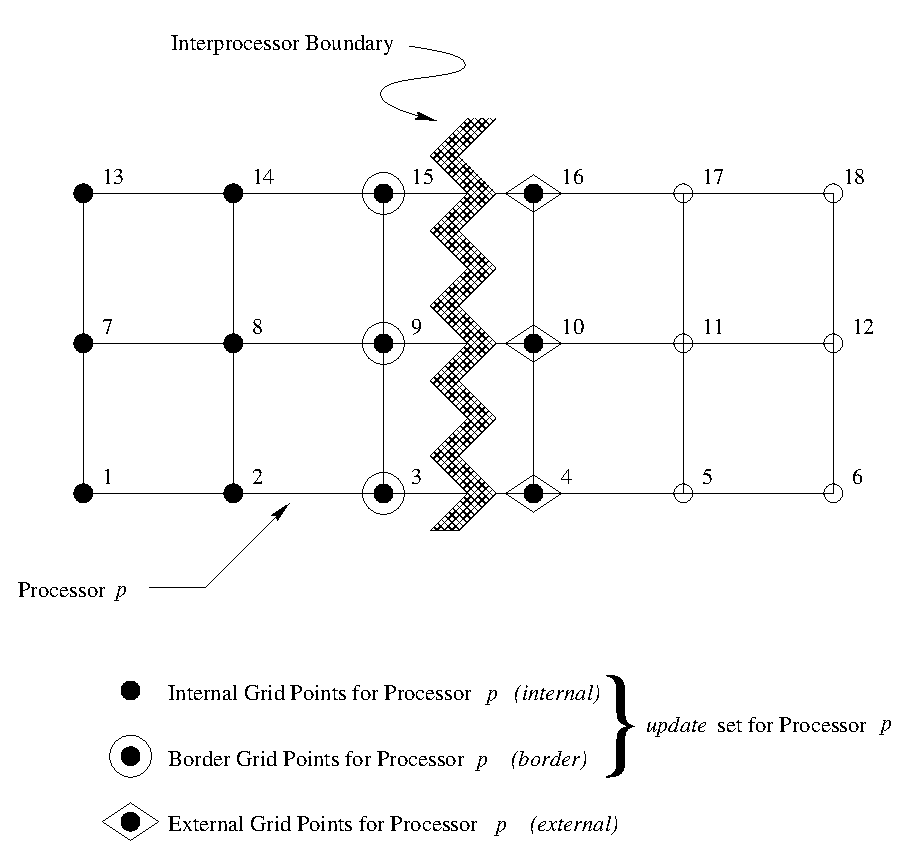
\epsfig{file=./figs/aztec_decomp.eps,height=4.5in,clip}}
      \vspace{0.5em}
    \end{minipage}}
  \caption{Example partitioning of a finite element grid.} \label{aztec_decomp}
\end{figure}
Since these sets of indices are used exclusively to reference specific vector
components, the same names (i.e., {\it update\/}, {\it internal\/}, {\it
  border\/} and {\it external\/}) are sometimes used below to describe the
vector elements themselves.  Having generalized these labels, the three types
of vector elements are distinguished by locally storing the {\it internal}
components first, followed by the {\it border} components and finally by the
{\it external} components.  In addition, all {\it external} components received
from the same processor are stored consecutively.  Below we summarize the
nomenclature for a processor with $N$ total elements where {\it N\_internal\/},
{\it N\_border\/}, and {\it N\_external\/} elements are distributed over the
sets {\it internal\/}, {\it border\/} and {\it external\/} respectively.
\vskip .2in
\begin{center}
  \begin{tabularx}{\textwidth}{|l|X|X|} \hline
    \bf set & \bf description & \bf local numbering \\ \hline \hline
    \it internal & updated w/o communication & $0$ to $ N\_internal - 1$.\\
    \hline
    \it border & updated with communication & $N\_internal$ to $N\_internal
    + N\_border - 1$. \\ \hline
    \it external & not updated but used to update \it border. & $N\_internal +
    N\_border$ to $N - 1$. Elements received from the same processor are
    numbered consecutively. \\ \hline
  \end{tabularx}
\end{center}
\vskip .2in

Similar to vectors, a subset of matrix non-zeros is stored on each processor.
In particular, each processor stores only those rows which correspond to its
{\it update\/} set.  For example, if vector element $i$ is updated on processor
$p$, then processor $p$ also stores all the non-zeros of row $i$ in the matrix.
Further, the local numbering of vector elements on a specific processor induces
a local numbering of matrix rows and columns.  For example, if vector element
$k$ is locally numbered as $k_l$, then all references to row $k$ or column $k$
in the matrix would be locally numbered as $k_l$.  Thus, each processor
contains a submatrix whose row and column entries correspond to variables
defined on this processor.

The remainder of this section describes the two sparse matrix formats that are
used to store the local renumbered submatrix. These two sparse matrix formats
correspond to common formats used in serial computations.

\subsection{Distributed Modified Sparse Row (DMSR) Format} \label{DMSR Format}

The DMSR format is a generalization of the MSR format~\cite{concurrency}. The
data structure consists of an integer vector {\it bindx\/} and a double
precision vector {\it val\/} each of length {\it N\_nonzeros + 1} where {\it
  N\_nonzeros} is the number of nonzeros in the local submatrix.  For a
submatrix with $m$ rows the DMSR arrays are as follows:
%
\vspace{2em}
%{\flushleft{\bf Descriptions} \hrulefill}
%\nopagebreak% \\[0.5em]
\begin{tabbing}
$\hphantom{rp}$
\= {\it bindx {\bf :}\/} \\[0.3em]
\>$\hphantom{rpntrsqv}$
  \= {\it bindx[0]\/} \hskip 0.9in \= = \= m + 1 \\
\>\> {\it bindx[k+1] - bindx[k]\/} \> = \> number of nonzero
                                           off-diagonal elements
                                           in {\it k\/}'th \\
\>\>                               \>   \> row, $k < m $ \\
\>\> {\it bindx[$k_s ... k_e$]\/}  \> = \> column indices of the
                                           off-diagonal
                                           nonzeros in row\\
\>\>                               \>   \> $k$ where
                                           $k_s$ = {\it bindx[k]} and
                                           $k_e$ = {\it bindx[k+1]-1}.\\[0.8em]
\> {\it val {\bf :}\/} \\[0.3em]
\>\> {\it val[k] \/}               \> = \> $ A_{kk}, k < m $ \\
\>\> {\it val[$k_i$] \/}   \> = \> the ($k$, {\it bindx[$k_i$] \/})'th
                                           matrix element where \\
\>\>                               \>   \> $k_s \leq k_i \leq k_e $
                                           with $k_s$ and $k_e$ as defined
                                           above.
\end{tabbing}
%
\vspace{1em}
Note: {\it val[m]\/} is not used. See~\cite{sparker2} for a detailed
discussion of the MSR format.

\subsection{Distributed Variable Block Row (DVBR) Format} \label{DVBR Format}

The Distributed Variable Block Row (DVBR) format is a generalization of the VBR
format~\cite{sparker2}.  The data structure consists of a double precision
vector {\it val\/} and five integer vectors: {\it indx\/}, {\it bindx\/}, {\it
  rpntr\/}, {\it cpntr\/} and {\it bpntr\/}.  The format is best suited for
sparse block matrices of the form
\[
A = \left( \begin{array}{cccc}
        A_{00} & A_{01} & \cdots & A_{0k} \\
        A_{10} & A_{11} & \cdots & A_{1k} \\
        \vdots & & \ddots & \vdots \\
        A_{m0} & \cdots & \cdots & A_{mk} \end{array}
\right)
\]
where $A_{ij}$ denotes a block (or submatrix). In a sparse block matrix, some
of these blocks would be entirely zero while others may be dense. The DVBR
vectors are described below for a matrix with $M \times K$ blocks.
%
\vspace{1em}
%{\flushleft{\bf Descriptions} \hrulefill}
%\nopagebreak %\\[0.5em]
\begin{tabbing}
$\hphantom{rp}$
\= {\it rpntr[0 ... M] {\bf :}\/} \\[0.3em]
\>$\hphantom{rpntrsqv}$
  \= {\it rpntr[0]\/} \hskip 0.9in \= = \= 0 \\
\>\> {\it rpntr[k+1] - rpntr[k]\/} \> = \> number of rows in {\it
                                           k\/}'th block row \\[0.8em]
\> {\it cpntr[0 ... K] {\bf :}\/} \\[0.3em]
\>\> {\it cpntr[0]\/}              \> = \> 0 \\
\>\> {\it cpntr[k+1] - cpntr[k]\/} \> = \> number of columns in {\it
                                           k\/}'th block column \\[0.8em]
\> {\it bpntr[0 ... M] {\bf :}\/} \\[0.3em]
\>\> {\it bpntr[0]\/}              \> = \> 0 \\
\>\> {\it bpntr[k+1] - bpntr[k]\/} \> = \> number of nonzero blocks in the
                                           {\it k\/}'th block row\\[0.8em]
\> {\it bindx[0 ... bpntr[M] - 1] {\bf :}\/}\\[0.3em]
\>\> {\it bindx[$k_s ... k_e$]\/}  \> = \> block column indices of nonzero
                                           blocks in block row $k$ \\
\>\>                               \>   \> where $k_s$ = {\it bpntr[k]} and
                                           $k_e$ = {\it bpntr[k+1]}-1 \\[0.8em]
\> {\it indx[0 ... bpntr[M] ] {\bf :}\/}\\[0.3em]
\>\> {\it indx[0]\/}               \> = \> 0 \\
\>\> {\it indx[$k_i$+1] - indx[$k_i$]\/}\> = \> number of nonzeros in
                                                the ($k$, {\it
                                                bindx[$k_i$]\/})'th
                                                block \\
\>\>                               \>   \> where $k_s \leq k_i \leq
                                           k_e$ with $k_s$ and $k_e$
                                           as defined \\
\>\>                               \>   \> above. \\[0.8em]
\> {\it val[0 ... indx[bpntr[M]] - 1 ] {\bf :}\/}\\[0.3em]
\>\> {\it val[$i_s ... i_e$]\/}  \> = \> nonzeros in the ($k$, {\it
     bindx[$k_i$]\/})'th block stored in \\
\>\>                             \>   \> column major order where
                                         $k_i$ is as defined above, \\
\>\>                             \>   \> $i_s$ = {\it indx[$k_i$]} and
                                         $i_e$ = {\it indx[$k_i$+1]}-1
\end{tabbing}
\vspace{1em}
%
See~\cite{sparker2} for a detailed discussion of the VBR format.

%%% Local Variables:
%%% mode: latex
%%% TeX-master: "az_ug_20"
%%% End:


\section{High Level Data Interface\label{highlevel_data_inter}}

Setting up the distributed format described in Section~\ref{data_formats} for
the local submatrix on each processor can be quite cumbersome. In particular,
the user must determine a mapping between the global numbering scheme and a
local scheme which facilitates proper communication.  Further, a number of
additional variables must be set for communication and synchronization (see
Section~\ref{advanced_topics}).  In this section we describe a simpler data
format that is used in conjunction with a transformation function to generate
data structures suitable for \Az{}.  The new format allows the user to specify
the rows in a natural order as well as to use global column numbers in the {\it
  bindx} array.  To use the transformation function the user supplies the {\it
  update\/} set and the submatrix for each processor.  Unlike the previous
section, however, the submatrix is specified using the global coordinate
numbering instead of the local numbering required by \Az{}. This procedure
greatly facilitates matrix specification and is the main advantage of the
transformation software.

On a given processor, the {\it update\/} set (i.e.  vector element assignment
to processors) is defined by initializing the array {\it update\/} on each
processor so that it contains the global index of each element assigned to the
processor. The {\it update} array must be sorted in ascending order (i.e. $ i <
j \Rightarrow update[i] < update[j]$). This sorting can be performed using the
\Az{} function {\sf AZ\_sort}. Matrix specification occurs using the arrays
defined in the previous section. However, now the local rows are defined in the
same order as the {\it update} array and column indices (e.g. {\it bindx}) are
given as global column indices.  To illustrate this in more detail, consider
the following example matrix:
\[
A = \pmatrix{ a_{00} & a_{01} &        & a_{03} & a_{04} &        \cr
              a_{10} & a_{11} &        & a_{13} &        &        \cr
                     &        & a_{22} & a_{23} & a_{24} & a_{25} \cr
              a_{30} & a_{31} & a_{32} & a_{33} & a_{34} & a_{35} \cr
              a_{40} &        & a_{42} & a_{43} & a_{44} &        \cr
                     &        & a_{52} & a_{53} &        & a_{55} } .
\]
Figure~\ref{init_input} illustrates the information corresponding to a
particular matrix partitioning that is specified by the user as input to the
data transformation tool.
\begin{figure}[Htbp]
  \shadowbox{
%    \begin{minipage}{\textwidth}
    \begin{minipage}{6.2in}
      \vspace{0.5em}
      {\large \flushleft{\bf Example}} \hrulefill %
      \vspace{0.5em}
%%%
\begin{tabbing}
\tt
\hsp proc 0: \\
\>  \hsp N\_update: \in  3 \\
\>  \>   update:    \>   0 \sp 1  \sp 3 \\
\>  \>   bindx:     \>   4       \>   7       \>   9       \sp 14     \sp 1
                    \sp  3       \sp  4       \sp  0       \sp  3     \sp  0
                    \sp  1       \sh  2       \sh  4       \sh  5\\
\>  \>   val:       \>  $a_{00}$ \>  $a_{11}$ \>  $a_{33}$ \> \hskip .05in -  \> $a_{01}$
                    \>  $a_{03}$ \>  $a_{04}$ \>  $a_{10}$ \> $a_{13}$\>$a_{30}$
                    \>  $a_{31}$ \bb $a_{32}$ \bb $a_{34}$ \bb $a_{35}$\\
\>-----------------------------------------------------------------------------------------------------------\\
\>  proc 1:\\
\>  \>   N\_update: \>   1\\
\>  \>   update:    \>   4\\
\>  \>   bindx:     \>   2 \>   5  \>   0 \>   3  \>  2 \\
\>  \>   val:       \>$a_{44}$\>\hskip .025in -\>$a_{40}$\>$a_{43}$\>$a_{42}$\\
\>-----------------------------------------------------------------------------------------------------------\\
\>  proc 2:\\
\>  \>   N\_update: \>   2\\
\>  \>   update:    \>   2 \>   5\\
\>  \>   bindx:     \>   3 \>   6  \>   8 \>   3  \>  4  \> 5  \> 2  \> 3\\
\>  \>   val:       \>$a_{22}$\>$a_{55}$\>\hskip .025in -\>$a_{23}$\>
                        $a_{24}$\>$a_{25}$\>$a_{52}$\>$a_{53}$
\end{tabbing}
%%%
      \vspace{0.5em}
    \end{minipage}}
  \caption{User input (MSR format) to initialize the sample matrix problem.}
  \label{init_input}
\end{figure}
%It should also be note that though this example
%considers only the sparsity pattern of the matrix, it is possible to
%specify the actual nonzero entries as well at the start of the calculation.
Using this information, {\sf AZ\_transform}
\begin{itemize}
\item determines the sets {\it internal}, {\it border} and
      {\it external}.
\item determines the local numbering:
      {\it update\_index[i]} is the local numbering for
      {\it update[i]} while {\it extern\_index[i]} is the local
      numbering for {\it external[i]}.
\item permutes and renumbers the local submatrix rows and columns so that
      they now correspond to the new ordering.
\item computes additional information
      (e.g. the number of internal, border and external components on this
      processor) and
      stores this in {\it data\_org\/} (see Section~\ref{advanced_topics}).
\end{itemize}
A sample transformation is given in Figure~\ref{init_mv_structs}
%
\begin{figure}[Htbp]
  \shadowbox{
%    \begin{minipage}{\textwidth}
    \begin{minipage}{6.2in}
      \vspace{0.5em}
      {\large \flushleft{\bf Example}} \hrulefill %
      \vspace{0.5em}
%%%
\begin{verbatim}
init_matrix_vector_structures(bindx, val, update, external,
                              update_index, extern_index, data_org);
{
  AZ_read_update(update, N_update);
  create_matrix(bindx, val, update, N_update);
  AZ_transform(bindx, val, update, external, update_index,
               extern_index, data_org, N_update);
}
\end{verbatim}
%%%
      \vspace{0.1em}
    \end{minipage}}
  \caption{{\sf init\_matrix\_vector\_structures}.}\label{init_mv_structs}
\end{figure}
%
and is found in the file \verb'az\_app\_utils.c'.  {\sf AZ\_read\_update} is an
\Az{} utility which reads a file and assigns elements to {\it update\/}.  The
user supplied routine {\sf create\_matrix} creates an MSR or VBR matrix using
the global numbering.  Once transformed the matrix can now be used within
\Az{}.

%%% Local Variables:
%%% mode: latex
%%% TeX-master: "az_ug_20"
%%% End:


\chapter{Examples} \label{sec:examples}

\section{Short Tutorial}

In this section, we write a driver code which calls the Mesquite
library to improve the quality of a test mesh. This tutorial section
is aimed at giving the user a feel for Mesquite: \emph{this section is not
where to look for detailed information}. In particular, information
pertaining to loading a particular mesh format (see Chapter \ref{sec:meshes}), 
interacting through a particular mesh interface (section \ref{sec:MeshData}), 
and details of defining geometric domains (see Chapter \ref{sec:geom}) are not
given in this section.

First, we write a small program using Mesquite's simplified API, or
wrappers, to show the fastest way to deploy Mesquite functionality to
improve a mesh.  The wrapper concept, as well as details about the
different wrappers available, are described in section
\ref{sec:tutWrapper}.  Following this first example, we set up customized mesh
improvement tool using Mesquite's low-level API, the details of which
are described in section \ref{sec:tutDetailedAPI}.

\subsection{Tutorial File Template}
\label{sec:tutfile}

To create and link a driver code, the Mesquite library must be
installed per the instructions of section \ref{sec:compiling}. 
The commands and file names specified in this section are relative 
to the installed \texttt{testsuite/tutorial} directory.  It 
is assumed that that is the working diretory.
This tutorial begins with the file \texttt{tutorial.cpp}, 
which contains the following template:
\begin{verbatim}
1.  #include "Mesquite_all_headers.hpp"
    #include <ostream>
2.  using namespace Mesquite;
    int main(int argc, char* argv[])
    {
3.    MsqError err;

      if (argc != 2) {
        std::cerr << "Expected mesh file names as single argument."
                  << std::endl;
        exit (EXIT_FAILURE);
      }

      // new code starts here
4.    //... 

      return 0;
    }
\end{verbatim}
The lines labeled 1-3 highlight three basic aspects of using Mesquite;
\begin{enumerate}
\item For convenience, Mesquite provides the header file
\begin{center}
\texttt{include/Mesquite\_all\_headers.hpp}
\end{center} which includes all Mesquite
headers. Although this is the easiest way to handle the include directives,
it may slow down compilation of the application.  
\item All Mesquite classes are part of the \texttt{Mesquite} namespace. 

\item  The \texttt{MsqError} class defines an object type used to communicate
Mesquite errors to the application.  The calling application must pass
an instance of the \texttt{MsqError} class or an instance of a subclass of
\texttt{MsqError} to many Mesquite functions.  The state of the error object
may be checked by casting the instance ot a Boolean or using it in a 
Boolean context.  The state is cleared by calling the \texttt{clear} method.
\item In the sections that follow, we guide the user through the steps
necessary to smooth a mesh using Mesquite.  All new lines of code to be
added to the template file start in this position and are added in the order
in which they are discussed.
\end{enumerate}

The code above takes a mesh file name as a command line argument and
performs no action. We can compile it in the 
(\texttt{examples/}) directory with the command:

\begin{verbatim}
                        make -f tutorial.make
\end{verbatim}


\subsection{Loading a Test Mesh}
\label{sec:tutMesh}
Our next step is to load one of the test meshes distributed with
Mesquite.  These meshes are distributed in the VTK unstructured mesh
format, the details of which are given in \cite{VTKbook, VTKuml}. This
format was chosen because of its readability and ease of use. 
In this tutorial we use
the simplest mechanism for loadling a mesh into Mesquite; different
options are described in Chapter \ref{sec:meshes}.  In particular, to
load a VTK test mesh in Mesquite, instantiate the Mesquite mesh
database object,
\texttt{MeshImpl}, and use the \texttt{read\_vtk} member function by
adding the following lines to the file template described in
\ref{sec:tutfile}.
\begin{verbatim}
  Mesquite::MeshImpl my_mesh;
  my_mesh.read_vtk(argv[1], err); 
  if (err) 
  {
    std::cout << err << std::endl;
    return 1;
  }
\end{verbatim}

If the mesh read in contains more than one type of element, Mesquite will automatically
handle the mixed elements with no additional effort required.

Mesquite also provides a function to write a mesh
file in VTK format, given a \texttt{MeshImpl} object:
\begin{verbatim}
  my_mesh.write_vtk("original_mesh.vtk",err); 
\end{verbatim}

Mesquite deals automatically with all types of supported elements 
(triangles, quadrilaterals, tetrahedra, hexahedra, wedges, and pyramids),
and also hybrid meshes consisting of mixed element types.  
Some meshes require geometry information as well.  When improving a surface mesh, Mesquite must be provided information
about surface(s) the mesh is constrained to lie on and the association between
mesh entities and entities of the geometric domain (surfaces, curves, etc.)
Because Mesquite is inherently a 3D code, all 2D meshes must specify some
geometry constraints.  The details
for general geometric surfaces are explained in Chapter 
\ref{sec:geom}. In this section,
we show how to define the geometry of a 2D planar mesh, specified by a
point $(x,y,z)$ and a normal. For example, the following defines an xy-plane
shifted five units in the z-direction:
\begin{verbatim}
  Vector3D normal(0,0,1);
  Vector3D point(0,0,5);
  PlanarDomain my_mesh_plane(normal, point);
\end{verbatim}


\subsection{Improving the Mesh with a Wrapper Class}
\label{sec:tutWrapper}
The simplest way to use a Mesquite mesh quality improvement
procedure is to instantiate one of the wrapper classes described in Chapter 
\ref{sec:wrappers}. Here, we will instantiate the
\texttt{LaplacianSmoother} wrapper and use it to improve 
the Mesh we created earlier.  Mesquite can optimize the mesh
without further input from the user by utilizing preset, default
values.  If some customization is desired, the wrapper classes also
allow users to set the most important parameters of the underlying
algorithms and metrics (see Chapter 
\ref{sec:wrappers} for details).
\begin{verbatim}
Mesquite::LaplaceWrapper mesh_quality_algorithm;

MeshDomainAssoc mesh_and_domain = MeshDomainAssoc(&my_mesh, &my_mesh_plane);
mesh_quality_algorithm.run_instructions(&mesh_and_domain, err);

//Should check the error object after the instruction is ran
// to see whether the instructions were all successful.
if (err) 
{
    std::cout << err << std::endl;
    return 1;
}
\end{verbatim}

Once the algorithm has been executed using the {\tt run\_instructions} member
function of the wrapper class, the improved mesh can be written to a new
file:
\begin{verbatim}
  my_mesh.write_vtk("smoothed_mesh.vtk",err); 
\end{verbatim}
This completes the code necessary for the simple wrapper example. Once
the code has successfully compiled by typing the {\tt make} command given in
section \ref{sec:tutfile}, 
run it from the tutorial directory \texttt{mesquite/testSuite/tutorial/}
with a mesh file name as a command line 
argument by typing: 
\begin{verbatim}
./tutorial ../../meshFiles/2D/VTK/square_quad_10_rand.vtk
\end{verbatim}
The code creates the files original\_mesh.vtk
and improved\_mesh.vtk in the current directory.  These two meshes, the
original and the optimized, are
shown in figure \ref{fig:square_rand}.  The text output of the code,
shown below, reports the inverse mean ratio quality metric statistics for
the orginal mesh before optimization and the final mesh after optimization.
The optimized mesh consists
of square quadrilaterals which have an inverse mean ratio value of 1.0.
\begin{verbatim}
************** QualityAssessor(free only) Summary **************

  Evaluating quality for 100 elements.
  This mesh had 100 quadrilateral elements.
  There were no inverted elements detected.
  No entities had undefined values for any computed metric.

     Element Quality Statistics

     minimum     average         rms     maximum     std.dev.
     1.01013     1.16655      1.1738     1.79134     0.130322

     Number of statistics = 100
     Metric = Inverse Mean Ratio
     Element Quality not based on sample points.


************** QualityAssessor(free only) Summary **************

  Evaluating quality for 100 elements.
  This mesh had 100 quadrilateral elements.
  There were no inverted elements detected.
  No entities had undefined values for any computed metric.

     Element Quality Statistics

     minimum     average         rms     maximum     std.dev.
           1           1           1     1.00001 2.20663e-006

     Number of statistics = 100
     Metric = Inverse Mean Ratio
     Element Quality not based on sample points.
\end{verbatim}
\begin{figure*}[htbp]
\begin{center}
    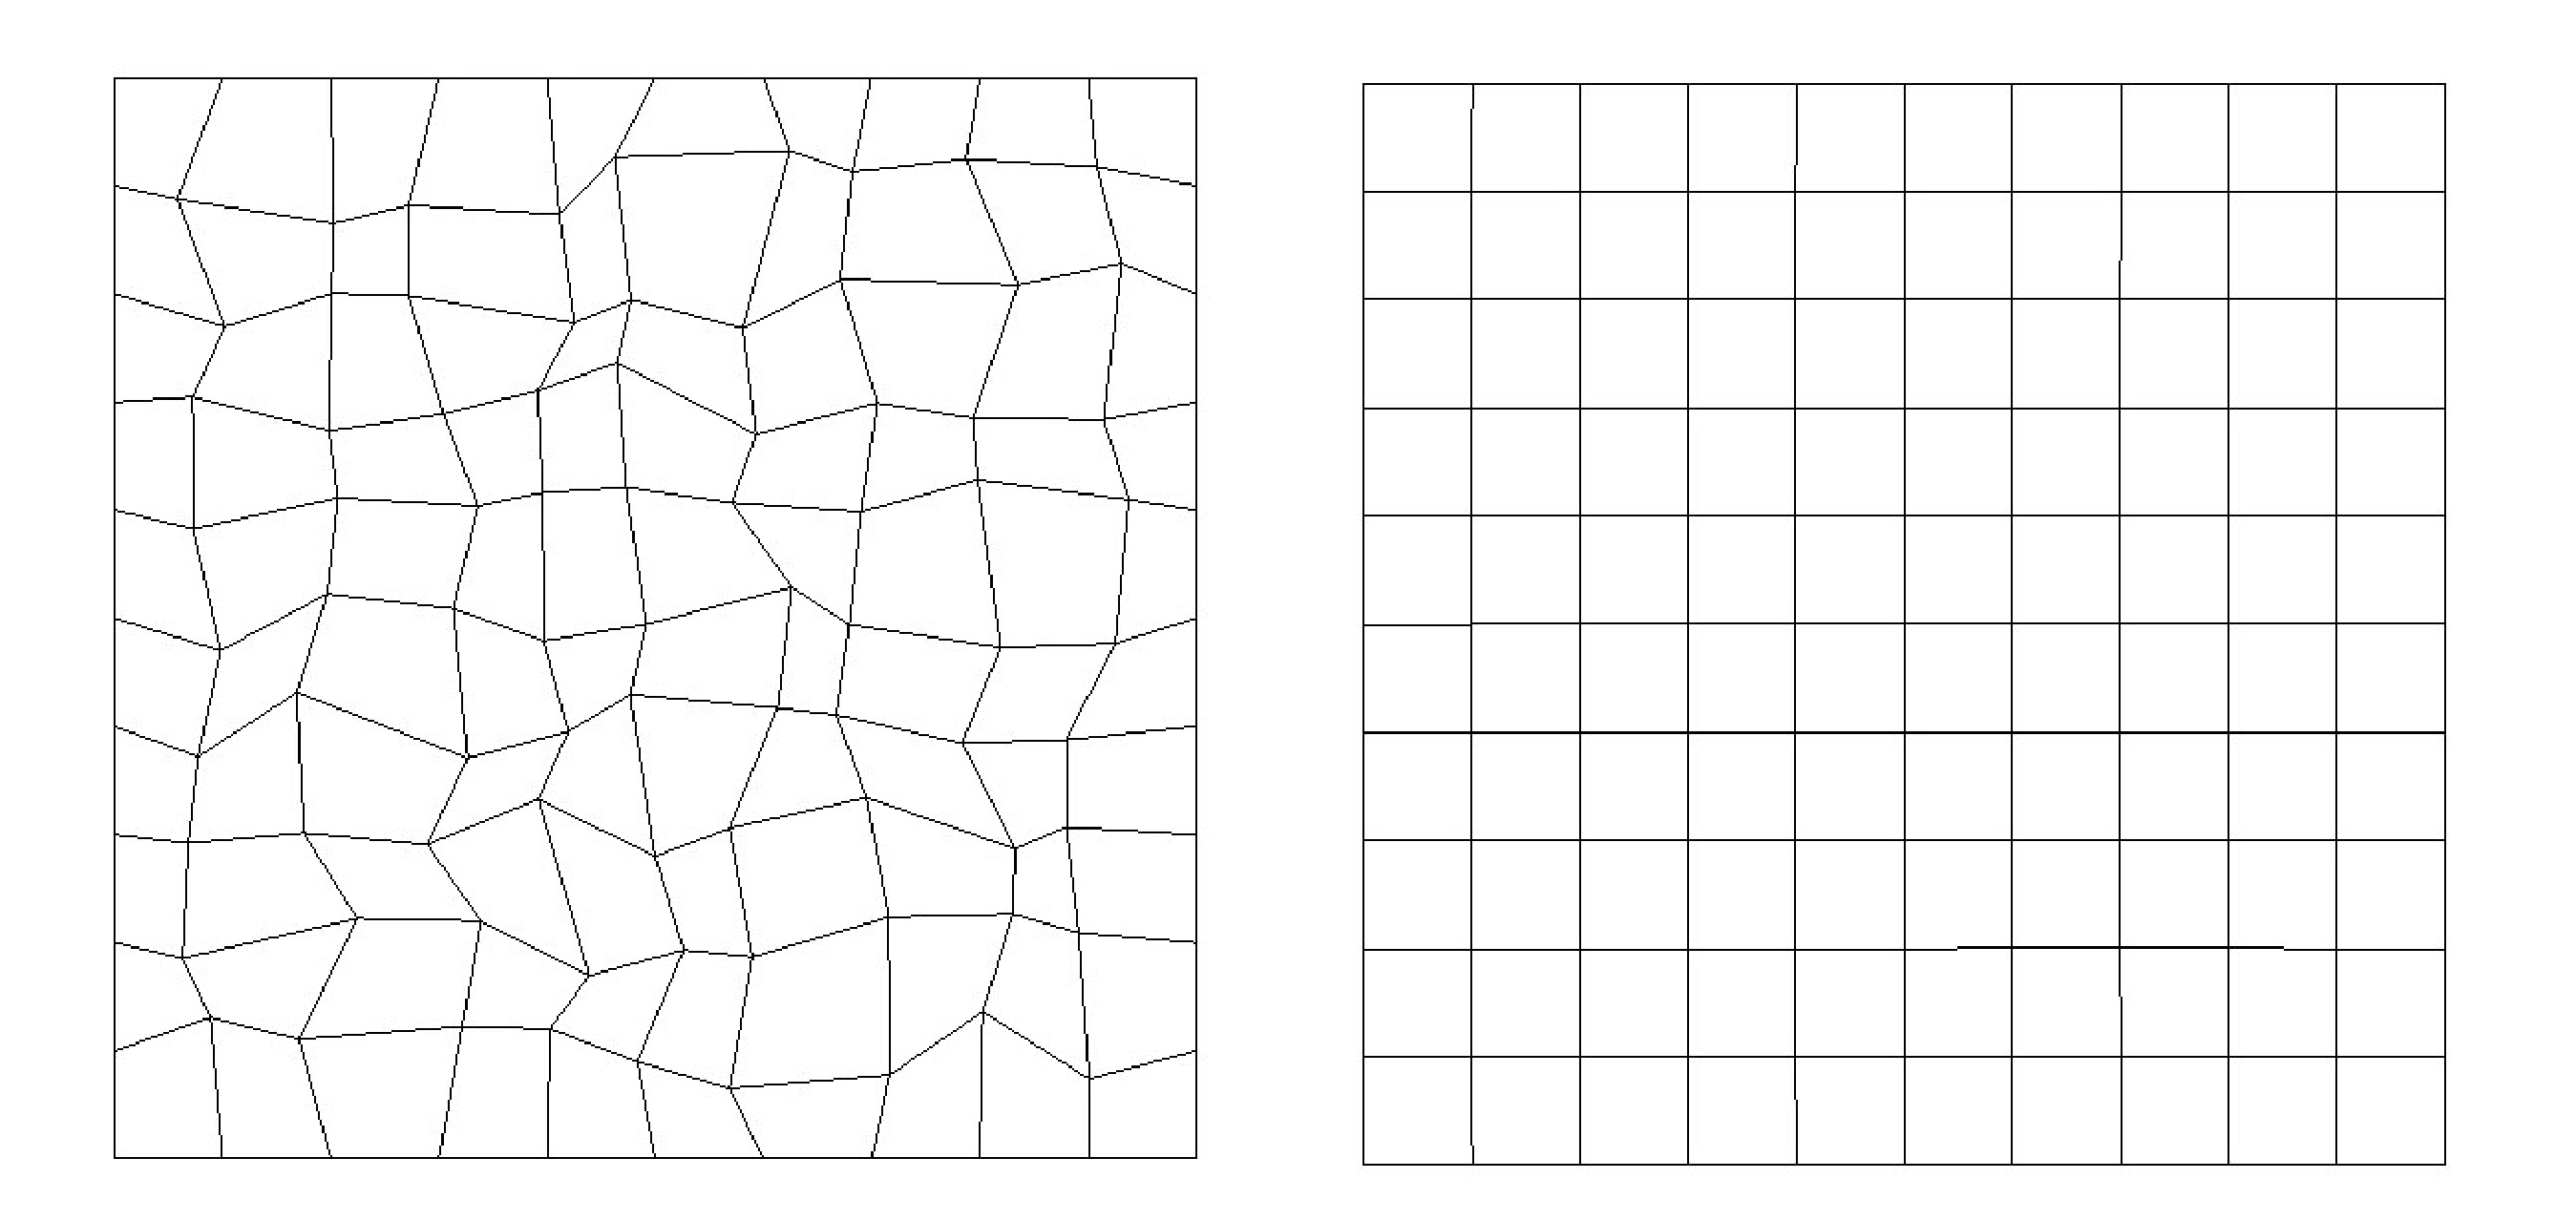
\includegraphics[height=80mm]{square_rand.eps}
    \caption{square\_quad\_10\_rand.vtk mesh. The original mesh is on the left, the mesh smoothed with the \texttt{LaplacianSmoother} is shown on the right.}
    \label{fig:square_rand}
\end{center}
\end{figure*}


\subsection{Improving the Mesh with the Low Level API}
\label{sec:tutDetailedAPI}
If the user requires in-depth control over the mesh quality improvement
process, the use of lower-level Mesquite classes provides an extensive
amount of flexibility.   In particular, the user can specify the quality
metric, objective function template, and optimization algorithm by
instantiating particular instances of each.  For each, various options
such as numerical or analytical gradient and Hessian evaluations or
the patch size can be selected.  Furthermore, the user can fine tune
the optimization algorithm performance by creating and setting the parameters 
of the termination criteria.
%for both inner and outer iterations.
%mbrewer removed reference to inner and outer iterations.
%{\tt LAF have we talked about inner and outer iterations before? perhaps
%too advanced for the tutorial}

Once these core objects have been created and customized, the user
creates an instruction queue and adds one or more quality improvers
and quality assessors to it.  The mesh optimization process is initiated
with the {\tt run\_instructions} method on the instruction queue
class.

In this section, we provide a simple example to highlight the main
steps needed for this approach.  The code segment given below performs
the same functionality as the wrapper class highlighted in the
previous section.  The comment lines provide high level documentation;
the details of each class and the low-level API are not described here.
%extensively treated in Section 
%\ref{sec:detailedAPI}.

\begin{verbatim}
    // creates a mean ratio quality metric ...
  IdealWeightInverseMeanRatio inverse_mean_ratio(err);

    // sets the objective function template
  LPtoPTemplate obj_func(&inverse_mean_ratio, 2, err);
  
    // creates the optimization procedures
  TrustRegion t_region(&obj_func);

    //performs optimization globally
  t_region.use_global_patch(); 

    // creates a termination criterion and 
    // add it to the optimization procedure
    // outer loop: default behavior: 1 iteration
    // inner loop: stop if gradient norm < eps
  TerminationCriterion tc_inner;
  tc_inner.add_absolute_gradient_L2_norm( 1e-4 ); 
  t_region.set_inner_termination_criterion(&tc_inner);

    // creates a quality assessor
  QualityAssessor m_ratio_qa(&inverse_mean_ratio);
    // creates an instruction queue
  InstructionQueue queue;
  queue.add_quality_assessor(&m_ratio_qa, err); 
  queue.set_master_quality_improver(&t_region, err); 
  queue.add_quality_assessor(&m_ratio_qa, err); 

    // do optimization of the mesh_set
  MeshDomainAssoc mesh_and_domain = MeshDomainAssoc(&my_mesh, &my_mesh_plane);
  queue.run_instructions(&mesh_and_domain, err);
  if (err) {
    std::cout << err << std::endl;
    return 2;
  }
\end{verbatim} 

\newpage

\subsection{Mesh Improvement Examples}

The left image in figure \ref{fig:hole} shows a mesh that has
been degraded by moving the disk from the right side of the square to
the left while keeping the mesh topology fixed.
The mesh file
\newline
\texttt{mesquite/meshFiles/2D/VTK/hole\_in\_square.vtk} contains the
information for this mesh.  If you plan to run this example, note that
the normal direction that defines the geometry is now $(0,0,-1)$.
This change must be made in the tutorial example code
as was done in section \ref{sec:tutMesh}, or an error message will be
thrown.
\begin{verbatim}
  Vector3D normal(0,0,-1);
  Vector3D point(0,0,-5);
  PlanarDomain my_mesh_plane(normal, point);
\end{verbatim}

We can now improve the mesh with the wrapper mentioned in
\ref{sec:tutWrapper} or the detailed API mentioned in
\ref{sec:tutDetailedAPI}. 
Because we changed the normal, the driver code must be recompiled;
otherwise the code and executable are as before.
Once the code is recompiled, type 
\begin{verbatim}
./tutorial ../../meshFiles/2D/VTK/hole_in_square.vtk
\end{verbatim}
to improve this mesh.
The smoothed mesh is shown in the right image of figure
\ref{fig:hole}.
The vertex locations have been repositioned and significantly improve
the quality of the mesh, as shown by the onscreen
quality assessor output:  
\begin{verbatim}
************** QualityAssessor(free only) Summary **************

  Evaluating quality for 140 elements.
  This mesh had 140 quadrilateral elements.
  There were no inverted elements detected.
  No entities had undefined values for any computed metric.

     Element Quality Statistics

     minimum     average         rms     maximum    std.dev.
     1.07588     85.8391     463.357     5037.46     455.336

     Number of statistics = 140
     Metric = Inverse Mean Ratio
     Element Quality not based on sample points.


************** QualityAssessor(free only) Summary **************

  Evaluating quality for 140 elements.
  This mesh had 140 quadrilateral elements.
  There were no inverted elements detected.
  No entities had undefined values for any computed metric.

     Element Quality Statistics

     minimum     average         rms     maximum    std.dev.
     1.01896     1.83479     1.91775     3.36336    0.557969

     Number of statistics = 140
     Metric = Inverse Mean Ratio
     Element Quality not based on sample points
\end{verbatim}
\begin{figure*}[htbp]
\begin{center}
    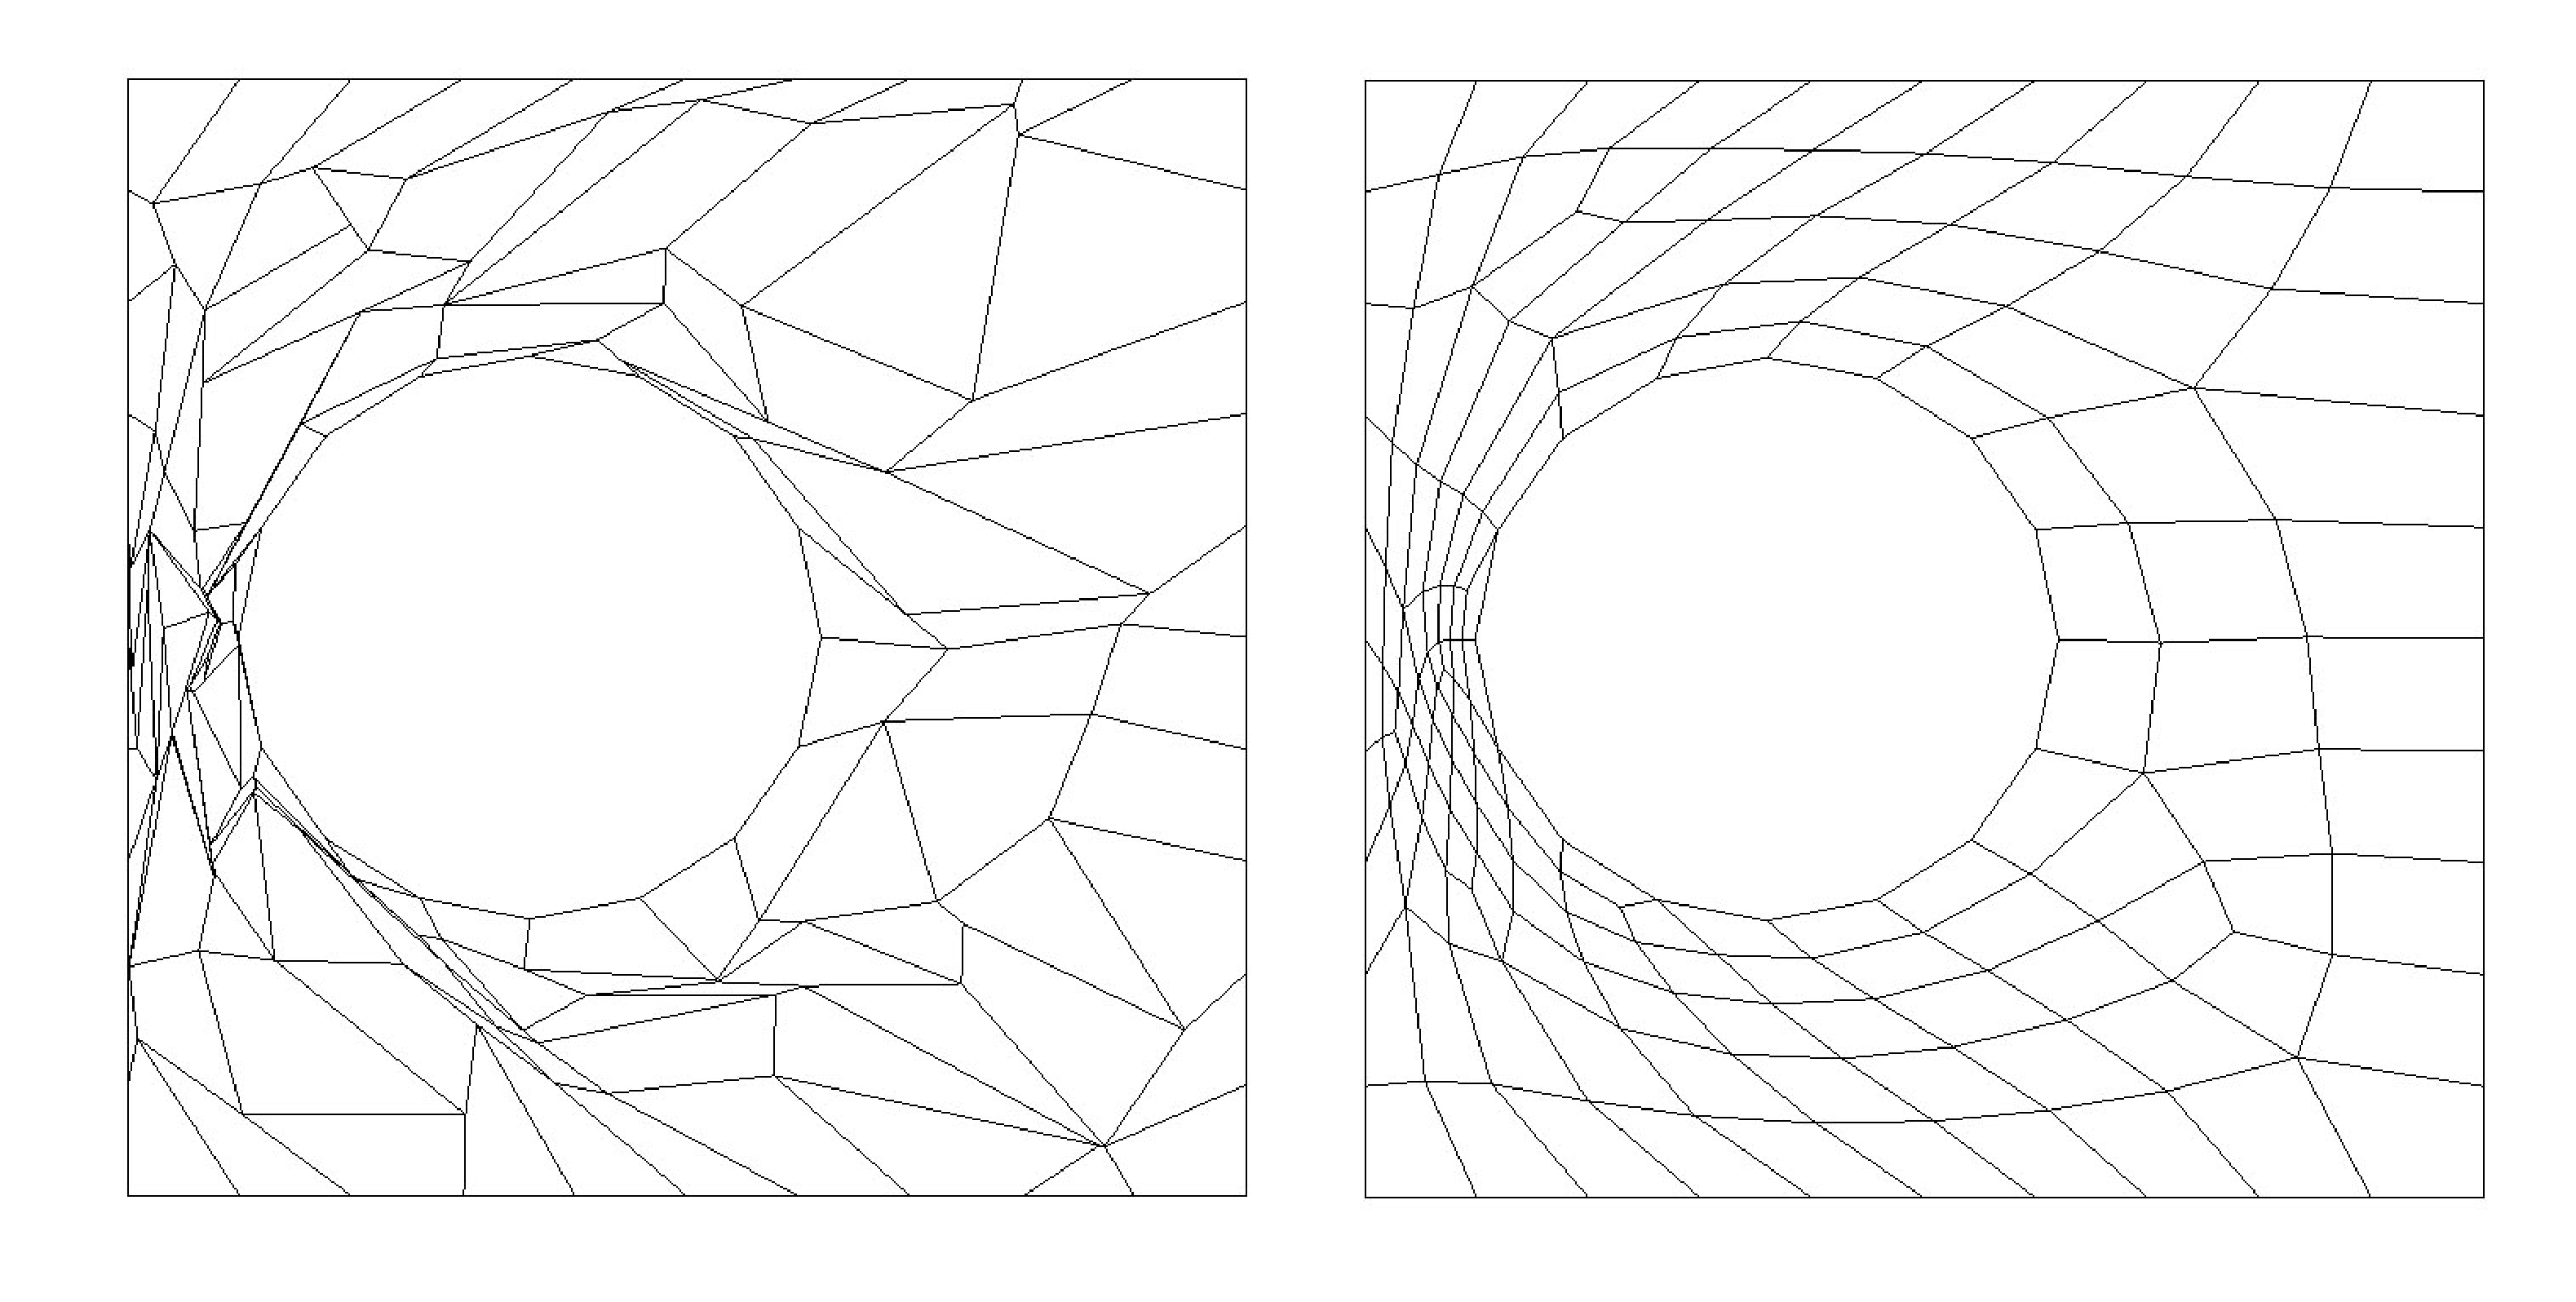
\includegraphics[height=80mm]{hole_in_square.eps}
    \caption{hole\_in\_square.vtk mesh. The original mesh is on the left, the mesh smoothed with
    Mesquite is shown on the right.}
    \label{fig:hole}
\end{center}
\end{figure*}


%%... section on testing ...

\subsection{Regression Testing}
\label{sec:RegressionTesting}
Regression testing encompasses
running unit tests as well as comparing results data against "blessed"
or "gold" data.  An example of comparing results of a smoothed mesh
against a gold version is in
\texttt{mesquite/testSuite/parallel\_smooth\_laplace/par\_hex\_smooth\_laplace.cpp}.
This utilizes a function in \texttt{MeshUtil}, \texttt{meshes\_are\_different}, to compare
two \texttt{MeshImpl} objects (within a specified numerical tolerance).  It is
recommended that both unit testing and gold-comparison testing be
included in your test code development.


\section{Advanced Topics\label{advanced_topics}}
\subsection{Data Layout\label{comm_vars}}
The \Az{} function {\sf AZ\_transform} initializes the integer array {\it
  data\_org}.  This array specifies how the matrix is set up on the parallel
machine.  In many cases, the user need not be concerned with the contents of
this array. However, in some situations it is useful to initialize these
elements without the use of {\sf AZ\_transform}, to access these array elements
(e.g. determine how many {\it internal} components are used), or to change
these array elements (e.g. when reusing factorization information, see
Section~\ref{reusing}). When using the transformation software, the user can
ignore the size of {\it data\_org} as it is allocated in {\sf AZ\_transform}.
However, when this is not used, {\it data\_org} must be allocated of size {\sf
  AZ\_COMM\_SIZE} $+$ number of vector elements sent to other processors during
matrix-vector multiplies.  The contents of {\it data\_org} are as follows:
\vspace{2em} {\flushleft{\bf Specifications} \hrulefill}
\nopagebreak \\[0.5em]
%
\optionbox{data\_org[{\sf AZ\_matrix\_type}]}{Specifies matrix
format.}
%
        \choicebox{AZ\_VBR\_MATRIX}{Matrix corresponds to VBR format.}
%
        \choicebox{AZ\_MSR\_MATRIX}{Matrix corresponds to MSR format.}
%
\optionbox{data\_org[{\sf AZ\_N\_internal}]}{Number of elements
                                      updated by this processor that
                                      can be computed without
                                      information from neighboring
                                      processors
                                      ({\it N\_internal\/}). This also
                                      corresponds to the number of internal
                                      rows assigned to this processor.}
%
\optionbox{data\_org[{\sf AZ\_N\_border}]}{Number of elements
                                      updated by this processor that
                                      use information from
                                      neighboring processors ({\it
                                      N\_border\/}).}
%
\optionbox{data\_org[{\sf AZ\_N\_external}]}{Number of {\it external}
                                      components needed by this
                                      processor ({\it
                                      N\_external\/}).}
%
\optionbox{data\_org[{\sf AZ\_N\_int\_blk}]}{Number of internal
                                      VBR block rows owned by this
                                      processor.  Set to
                                      data\_org[{\sf AZ\_N\_internal}]
                                      for MSR matrices.  }
%
\optionbox{data\_org[{\sf AZ\_N\_bord\_blk}]}{Number of border VBR block
                                      rows owned by this processor.
                                      Set to
                                      data\_org[{\sf AZ\_N\_border}]
                                      for MSR matrices.  }
%
\optionbox{data\_org[{\sf AZ\_N\_ext\_blk}]}{Number of external VBR
                                      block rows on this
                                      processor.  Set to
                                      data\_org[{\sf AZ\_N\_external}]
                                      for MSR matrices.  }
%
\optionbox{data\_org[{\sf AZ\_N\_neigh}]}{Number of processors with
                                      which we exchange information
                                      (send or receive) in performing
                                      matrix-vector products.}
%
\optionbox{data\_org[{\sf AZ\_total\_send}]}{Total number of vector
                                      elements sent to other processors
                                      during matrix-vector products.}
%
\optionbox{data\_org[{\sf AZ\_name}]}{Name of the matrix. This
                                      name is utilized when deciding
                                      which previous factorization to
                                      use as a preconditioner (see
                                      Section~\ref{reusing}).
                                      (positive integer value).}
%
\optionbox{data\_org[{\sf AZ\_neighbors}]}{Start of vector containing
                                      node i.d.'s of neighboring
                                      processors.  That is, {\it
                                      data\_org[{\sf
                                      AZ\_neighbors}+i]\/} gives the
                                      node i.d. of the ({\it
                                      i+1\/})'th neighbor.}
%
\optionbox{data\_org[{\sf AZ\_rec\_length}]}{Start of vector containing
                                      the number of elements to
                                      receive from each neighbor.
                                      We receive from the ({\it
                                      i+1\/})'th neighbor {\it
                                      data\_org[{\sf AZ\_rec\_length}+i]\/}
                                      elements.}
%
\optionbox{data\_org[{\sf AZ\_send\_length}]}{Start of vector containing
                                      the number of elements to send
                                      to each neighbor. We send to the
                                      ({\it i+1\/})'th neighbor {\it
                                      data\_org[{\sf AZ\_rec\_length}+i]\/}
                                      elements.}
%
\optionbox{data\_org[{\sf AZ\_send\_list}]}{Start of vector indicating the
                                      elements that we will send to
                                      other processors during
                                      communication. The first {\it
                                      data\_org[{\sf AZ\_send\_length}]\/}
                                      components correspond to the
                                      elements for the first neighbor
                                      and the next {\it
                                      data\_org[{\sf AZ\_send\_length}+1]\/}
                                      components correspond to element
                                      indices for the second neighbor,
                                      and so on.} $\hphantom{hi}$
%
\subsection{Reusing factorizations}\label{reusing}
By solving a problem with {\it options[{\sf AZ\_keep\_info}]} set to '1', 
\Az{} will not remove information so that it can be reused
later. In most cases, this information corresponds to either matrix scaling
factors or preconditioning factorization information for LU or ILU.  This
information is saved internally and referenced by the matrix name given by {\it
  data\_org[{\sf AZ\_name]}}. By changing {\it options[{\sf AZ\_pre\_calc}]}
and {\it data\_org[{\sf AZ\_name}]} a number of different \Az{} possibilities
can be realized. As an example, consider the following situation. A user needs
to solve the linear systems in the order shown below:
\[
A_1 x = b , A_2 y = x , \mbox{ and } A_1 z = y.
\]
The first and second systems are solved with {\it options[{\sf AZ\_pre\_calc}]}
set to {\sf AZ\_calc}. However, the name (i.e. {\it data\_org[{\sf AZ\_name}]})
is changed between these two solves. In this way, scaling and preconditioning
information computed from the first solve is not overwritten during the second
solve.  By then setting {\it options[{\sf AZ\_pre\_calc}]} to {\sf AZ\_reuse}
and {\it data\_org[{\sf AZ\_name}]} to the name used during the first solve,
the third system is solved reusing the scaling information (to scale the right
hand side, initial guess, and rescale the final solution\footnote{The matrix
  does not need to be rescaled as the scaling during the first solve overwrites
  the original matrix.}) and the preconditioning factorizations (e.g. ILU) used
during the first solve. While in this example the same matrix system is solved
for the first and third solve, this is not necessary. In particular,
preconditioners can be reused from previous nonlinear iterates even though the
linear system being solved are changing. Of course, many times information from
previous linear solves is not reused. In this case the user must explicitly
free the space associated with the matrix or this information will remain
allocated for the duration of the program. Space is cleared by invoking {\sf
  AZ\_free\_memory({\it data\_org[{\sf AZ\_name}]})}.

\subsection{Important Constants}
\Az{} uses a number of constants which are defined in the file
\verb'az_aztec_defs.h'. Most users can ignore these constants.  However, there
may be situations where they should be changed.  Below
is a list of these constants with a brief description:\\[2em]
\choicebox{AZ\_MAX\_NEIGHBORS}{Maximum number of processors with which
  information can be exchanged during matrix-vector products.}
\choicebox{AZ\_MSG\_TYPE\\ AZ\_NUM\_MSGS}{All message types used inside \Az{}
  lie between AZ\_MSG\_TYPE and AZ\_MSG\_TYPE + AZ\_NUM\_MSGS - 1.}
\choicebox{AZ\_MAX\_BUFFER\_SIZE}{Maximum message information that can be sent
  by any processor at any given time before receiving. This is used to
  subdivide large messages to avoid buffer overflows.}
\choicebox{AZ\_MAX\_MEMORY\_SIZE}{Maximum available memory.  Used primarily for
  the LU-factorizations where a large amount of memory is first allocated and
  then unused portions are freed after factorization.}
\choicebox{AZ\_TEST\_ELE}{Internal algorithm parameter that can effect the
  speed of the {\sf AZ\_find\_procs\_for\_externs} calculation.  Reduce {\sf
    AZ\_TEST\_ELE} if communication buffers are exceeded during this
  calculation.}  $\hphantom{h}$

\subsection{{\sf AZ\_transform} Subtasks}\label{subtasks}
The function {\sf AZ\_transform} described in
Section~\ref{highlevel_data_inter} is actually made up of 5 subtasks. In most
cases the user need not be concerned with the individual tasks. However, there
might arise situations where additional information is available such that some
of the subtasks can be omitted. In this case, it is possible for the user to
edit the code for {\sf AZ\_transform} located in the file \verb'az_tools.c' to
suit the application.  In this section we briefly describe the five subroutines
which make up the transformation function.  More detailed descriptions are
given in~\cite{aztec-utils}.  Prototypes for these subroutines as well as for
{\sf AZ\_transform} are given in Section~\ref{subroutines}.

{\sf AZ\_transform} begins by identifying the {\it external} set needed by each
processor.  Here, each column entry must correspond to either an element
updated by this processor or an {\it external} component.  The function {\sf
  AZ\_find\_local\_indices} checks each column entry.  If a column is in {\it
  update\/}, its number is replaced by the appropriate index into {\it
  update\/} (i.e. {\it update[new column index]\/} = old column index).  If a
column number is not found in {\it update\/}, it is stored in the {\it
  external} list and the column number is replaced by an index into {\it
  external\/} (i.e.  {\it external[new column index - N\_update]\/} = old
column index).

{\sf AZ\_find\_procs\_for\_externs} queries the other processors to determine
which processors update each of its {\it external} components. The array {\it
  extern\_proc\/} is set such that {\it extern\_proc[i]\/} indicates which
processor updates {\it external[i]\/}.

{\sf AZ\_order\_ele} reorders the {\it external} components such that elements
updated by the same processor are contiguous. This new ordering is given by
{\it extern\_index\/} where {\it extern\_index[i]\/} indicates the local
numbering of {\it external[i]\/}.  Additionally, {\it update} components are
reordered so the {\it internal} components precede the {\it border} components.
This new ordering is given by {\it update\_index\/} where {\it
  update\_index[i]\/} indicates the local numbering of {\it update[i]\/}.

{\sf AZ\_set\_message\_info} initializes {\it data\_org\/} (see
Section~\ref{comm_vars}) This is done by computing the number of neighbors,
making a list of the neighbors, computing the number of values to be sent and
received with each neighbor and computing the list of elements which will be
sent to other processors during communication steps.

Finally, {\sf AZ\_reorder\_matrix} permutes and reorders the matrix nonzeros so
that its entries correspond to the newly reordered vector elements.



\section{Matrix-Free Capabilities \label{matrix.free}}
Version 2.1 contains a matrix-free capability.  However, 
this capability is still undergoing some changes. 
In this document we describe the \Az{} interface
and give concrete examples with user-defined matrix-vector
products and user-defined preconditioners.
At present, only the `C' interface
has been completed. A Fortran interface will follow.

\subsection{{ AZ\_iterate}\label{interface}}

To use \Az{}'s solvers, a subroutine driver entitled {\it AZ\_iterate}
must be invoked. For those familiar with \Az{}{\bf 1.1}, this subroutine
replaces {\it AZ\_solve}. It should be noted that:
\begin{itemize}
\item {\it AZ\_solve} may still be used (when matrix-free is not needed).
%\item matrix-free capabilities can only be accessed via {\it AZ\_iterate}.
%\item {\it AZ\_iterate} is a superset of {\it AZ\_solve}. 
%That is, all the capabilities within {\it AZ\_solve} are available 
%via {\it AZ\_iterate}.
%\item {\it AZ\_iterate} will eventually replace {\it AZ\_solve}. 
%That is,
%      in the future {\it AZ\_solve} will no longer be supported.
\item The interface to {\it AZ\_iterate} will probably change a bit to
      incorporate new developments (including the integration of \Az{}
      with eigenvalue solvers and multilevel solvers).
\end{itemize}
There are three conceptual differences between {\it AZ\_iterate} and 
{\it AZ\_solve}:
\begin{itemize}
\item the user's matrix is more generalized and is now passed through a structure,
\item user-supplied preconditioning can be used,
\item {\bf two different matrices} can be supplied: one to solve
      and one to use within preconditioning. For example, \Az{}
      can solve equations $A x = f $ by applying an incomplete 
      factorization to a matrix $B$ which is 
      a sparse approximation to $A$.
\end{itemize}
The syntax for {\it AZ\_iterate} is given below.
%%%%%%%%%%%%%%%%%%%%%%%%%%%%%%%%%%%%%%%%%%%%%%%%%%%%%%%%%%%%%%%%%%%%%%%%%%%%%%%%
%
\protobox{void AZ\_iterate(double *{\it x\/}, double *{\it b\/}, int
*{\it options\/}, double *{\it params\/}, double *{\it status\/}, \\
$\hphantom{void AZ_iterate(}$ int *{\it proc\_config\/}, AZ\_MATRIX
*{\it Amat\/},
AZ\_PRECOND *{\it prec\/}, \\
$\hphantom{void AZ_iterate(}$ struct AZ\_SCALING *{\it scaling\/})}

\vspace{2em}
{\flushleft{\bf Parameters} \hrulefill}
\vspace{1em}

\optionbox{x, b, options, params, \\
           status, proc\_config}{These parameters are identical to those
           in {\it AZ\_solve} and are described in Section \ref{subroutines}.}

\optionbox{Amat}{On input, a structure representing the matrix to be
           solved (described below).}

\optionbox{prec}{On input, either NULL (implying \Az{}'s preconditioners
           are applied to {\it Amat}) or a structure indicating 
           the preconditioning routine and matrix to which preconditioning
           is applied (described below).}

\optionbox{scaling}{Currently not used.}

\vskip .1in
To complete the discussion, we must describe
how $Amat$ and $prec$ are created and set.
\subsection{Matrix-vector product examples.} 
The following examples use a variety of functions: 
{\it AZ\_set\_MSR()}, {\it AZ\_set\_VBR()}, etc.
%{\it AZ\_set\_MATFREE()},
%{\it AZ\_matrix\_create()}, 
%{\it AZ\_matrix\_destroy()},
%and 
%{\it AZ\_get\_matvec\_data ()}.
These functions are more fully described in Section \ref{subroutines}.
\vskip .1in
\underline{Example 1: DMSR or DVBR matrices}
\vskip .1in
\noindent
{\it AZ\_solve}() users with DMSR matrices can convert to {\it AZ\_iterate}()
by replacing 
\begin{verbatim}
   AZ_solve(x, b, options, params, indx, bindx, rpntr, cpntr, bpntr, 
            val, data_org, status, proc_config);
\end{verbatim}
with
\begin{verbatim}
   AZ_MATRIX *Amat;
      .
      .
   Amat = AZ_matrix_create(data_org[AZ_N_internal] +
                           data_org[AZ_N_border]);
   AZ_set_MSR(Amat, bindx, val, data_org, 0, NULL, AZ_LOCAL);
   AZ_iterate(x, b, options, params, status, proc_config, Amat, NULL, NULL);
   AZ_matrix_destroy(&Amat);
\end{verbatim}
Users with DVBR matrices  would replace {\it AZ\_set\_MSR()} by
\begin{verbatim}
    AZ_set_VBR(Amat, rpntr, cpntr, bpntr, indx, bindx,
               val, data_org, 0, NULL, AZ_LOCAL);
\end{verbatim}
\vskip .3in
\underline{Example 2: user-supplied matrix-vector product}
\vskip .1in
\noindent
This case is almost identically to the DMSR or DVBR examples
above except that {\it AZ\_set\_MATFREE} 
(as opposed to {\it AZ\_set\_MSR} or {\it AZ\_set\_VBR})
is used to associated
the user-defined matrix-vector product with the matrix.
\begin{verbatim}
   AZ_MATRIX *Amat;
      .
      .
   Amat = AZ_matrix_create(N_equations);
   AZ_set_MATFREE(Amat, my_data, my_matvec);
   AZ_iterate(x, b, options, params, status, proc_config, Amat, NULL, NULL);
   AZ_matrix_destroy(&Amat);
\end{verbatim}
{\tt N\_equations} is the number of matrix rows implicitly
kept on this processor (i.e. the length of the vector 
$y_{\mbox{\scriptsize local}}$ after performing 
$ y_{\mbox{\scriptsize local}} =  A_{\mbox{\scriptsize local}} 
x_{\mbox{\scriptsize local}}$). 
{\tt my\_data} is a user-defined data pointer that will be passed to
the user-defined matrix-vector product function {\tt my\_matvec}.
{\tt my\_matvec} should have the following proto-type:
\begin{verbatim}
void my_matvec(double *p, double *ap, AZ_MATRIX *Amat, int proc_config[])
\end{verbatim}
where

\optionbox{p}{On input, {\it p\/} is a vector containing local vector
              components for this processor. NOTE: \Az{}'s internal
              matrix-vector multiplies require additional space 
              (see {\it AZ\_solve}() description in Section \ref{subroutines}).}
\optionbox{ap}{On output, {\it ap\/} is set to $ (Amat)*p $.}
\optionbox{Amat}{On input, structure representing matrix 
                       used in matrix-vector multiplication.}
\optionbox{proc\_config}{On input, {\it proc\_config}[{\sf AZ\_node}] is 
                       set via the command {\it AZ\_set\_proc\_config }. }
Whenever the user-defined data pointer, {\it my\_data}, is needed inside 
{\it my\_matvec}(), it can be obtained via the function 
{\it AZ\_get\_matvec\_data (Amat)}.

\subsection{Preconditioning examples.} 
The following examples use: 
{\it AZ\_precond\_create()}, 
and 
{\it AZ\_precond\_destroy()}.
These functions are more fully described in Section \ref{subroutines}.
\vskip .1in
\underline{Example 1: Standard \Az{} preconditioning}
\vskip .1in
\noindent
Standard \Az{} preconditioning can be invoked 
by creating a preconditioner,
\begin{verbatim}
   AZ_PRECOND *prec;
      .
      .
   prec = AZ_precond_create(Amat, AZ_precondition, NULL);,
\end{verbatim}
passing it to {\it AZ\_iterate}(),
\begin{verbatim}
   AZ_iterate(x, b, options, params, status, proc_config, Amat, prec, NULL);,
\end{verbatim}
and finally clearing it with
\begin{verbatim}
   AZ_precond_destroy(&prec);
\end{verbatim}
\vskip .3in
\underline{Example 2: Standard \Az{} preconditioning applied to $B$}
\vskip .1in
\noindent
\Az{}'s preconditioners can be applied to a matrix, $B$, which is
different from the matrix being solved. In this case, the following
might be used:
\begin{verbatim}
   AZ_PRECOND *prec;
   AZ_MATRIX  *Amat, *Bmat;
      .
      .
   N_equations = data_org[AZ_N_internal]+data_org[AZ_N_border];
   Amat = AZ_matrix_create(N_equations);
   AZ_set_MSR(Amat, bindx, val, data_org, 0, NULL, AZ_LOCAL);
   Bmat = AZ_matrix_create(N_equations);
   AZ_set_MSR(Bmat, bindx2, val2, data_org2, 0, NULL, AZ_LOCAL);
   prec = AZ_precond_create(Bmat, AZ_precondition, NULL);
   AZ_iterate(x, b, options, params, status, proc_config, Amat, prec, NULL);
   AZ_matrix_destroy(&Amat);
   AZ_matrix_destroy(&Bmat);
   AZ_precond_destroy(&prec);
\end{verbatim}
\vskip .3in
\underline{Example 3: user-supplied preconditioner}
User-supplied preconditioning requires that the user's function pointer
and data pointer be given to {\sf AZ\_precond\_create()}.
For example,
\begin{verbatim}
   AZ_PRECOND *prec;
   AZ_MATRIX  *Amat;
      .
      .
   N_equations = data_org[AZ_N_internal]+data_org[AZ_N_border];
   Amat = AZ_matrix_create(N_equations);
   AZ_set_MSR(Amat, bindx, val, data_org, 0, NULL, AZ_LOCAL);
   prec = AZ_precond_create(Amat, my_preconditioner, my_data);
   AZ_iterate(x, b, options, params, status, proc_config, Amat, prec, NULL);
   AZ_matrix_destroy(&Amat);
   AZ_precond_destroy(&prec);
\end{verbatim}
{\tt my\_data} is a user-defined data pointer that will be passed to
the user-defined preconditioner function {\tt my\_preconditioner}.
{\tt my\_preconditioner} should have the following proto-type:
\begin{verbatim}
void my_preconditioner(double *z, int *options, int *proc_config, 
                       double *params, AZ_MATRIX *Amat, 
                       AZ_PRECOND *prec)
\end{verbatim}
where
\optionbox{z}{On input, {\it z\/} is a vector containing all the local vector
              components for this processor. On output, {\it z\/} is the
              preconditioned vector (local components).}

\optionbox{options, proc\_config\\
params, Amat, prec }{Same as those given to {\it AZ\_iterate}.}


\subsection{\Az{} preconditioning with user-defined matrices.} 
In general, \Az{} needs to know something about the matrix
in order to apply a preconditioner (see Table 1).
\vskip .1in
\noindent
%\begin{table}[h]
\begin{tabular}{|ll|}
\hline 
Preconditioner    & needed matrix information \\[9pt] \hline
Jacobi            & matrix diagonal \\
least squares  polynomial   & infinity norm of matrix \\
Neumann polynomial & infinity norm of matrix \\
incomplete  factorizations & algebraic preconditioners are used for the  subdomain\\
                  & solvers. These algebraic preconditioners need \\
                  & matrix entries.  \\
\hline 
\end{tabular}
\begin{center}
Table 1: {\it Data requirements for various preconditioners.}
\end{center}
\vskip .1in
%\caption{Data requirements of various preconditioners.\label{requirements}}
%\end{table}
For the polynomial preconditioners, it is possible to give \Az{}
the infinity norm via the command {\sf AZ\_set\_MATFREE\_matrix\_norm()}.
For Jacobi preconditioning it is often possible to give the 
matrix diagonal in a separate DMSR matrix. However, for most of the
other preconditioners, it is necessary to give all the matrix 
information.  The current \Az{} contains an experimental `getrow'
facility which allows this to be done. This `getrow' is demonstrated
in the example program \verb'az_mat_free_main.c' but is not officially
released as it is still undergoing changes.

%%%%%%%%%%%%%%%%%%%%%%%%%%%%%%%%%%%%%%%%%%%%%%%%%%%%%%%%%%%%%%%%%%%%%%%%%%%%%%%%

%\vspace{2em}
%
%\section{Compiling and Linking\label{comp_link}}
%
%The krylov solver library {\bf Aztec} uses code from a few publicly
%available linear algebra packages.  These packages are 1) the basic
%linear algebra subroutine library - BLAS  2) the linear algebra
%package - LAPACK and 3) a sparse direct lu solver Y12M. These packages
%can be obtained form netlib as described below.
%
%The following packages are needed by {\bf Aztec}:
%\begin{itemize}
%\item Y12M (used for LU factorizations)
%\item LAPACK routines
%\item BLAS   routines
%\end{itemize}
%These routines can be obtained via netlib.
%Send email to netlib@ornl.gov with the following information
%in the message:
%\vskip .5in
%\begin{verbatim}
%send help
%send index for y12m
%send index for lapack
%send index for blas
%\end{verbatim}
%\vskip .5in
%
%Current information on compiling and linking {\bf Aztec}
%for supported machines can be found in the file \verb'README'
%in the source code distribution directory.
%
%To obtain the {\bf Aztec} distribution send an email request to
%Ray S. Tuminaro (tuminaro@cs.sandia.gov).


%\newpage
%\bibliographystyle{plain}
%\bibliography{aztec_guide}
%
%
%\end{document}


%
% Command to put backslashes in front of underscores
%             :1,$s/\([^\\]\)\_/\1\\_/g
%    actually this changes a couple of lines within math symbols
%    like $P_t$.
%
\section{\ML\ Functions \label{subroutines}}

%%%%%%%%%%%%%%%%%%%%%%%%%%%%%%%%%%%%%%%%%%%%%%%%%%%%%%%%%%%%%%%%%%%%%%%%%%%%%%%

\addcontentsline{toc}{subsection}{AZ\_ML\_Set\_Amat}
\protobox{int AZ\_ML\_Set\_Amat(ML *ml\_object, int k, int isize, int osize, AZ\_MATRIX *Amat,\\
 \phantom{int AZ\_ML\_Set\_Amat(}int *proc\_config)}

\vspace{2em}
{\flushleft{\bf Description} \hrulefill}
\vspace{1em}

Create an \ML\  matrix view of an existing \Aztec matrix and store it within the `ml\_object'
context.


\vspace{2em}
{\flushleft{\bf Parameters} \hrulefill}
\vspace{1em}

\optionbox{ml\_object}{On input, \ML\  object pointer (see ML\_Create). On output, the
                      discretization matrix of level k is the same as given by Amat.}

\optionbox{k}{On input, indicates level within ml\_object hierarchy (should be between
                  0 and Nlevels${}^\dagger$-1).}

\optionbox{isize}{On input, the number of local rows in the submatrix stored on this
                  processor.}

\optionbox{osize}{On input, the number of columns in the local submatrix stored on this
                       processor not including any columns associated with ghost unknowns.}

\optionbox{Amat}{On input, an \Aztec data structure representing a matrix.
                       See the \Aztec User's Guide.}

\optionbox{proc\_config}{On input, an \Aztec data structure representing processor information.
                       See the \Aztec User's Guide.}


%%%%%%%%%%%%%%%%%%%%%%%%%%%%%%%%%%%%%%%%%%%%%%%%%%%%%%%%%%%%%%%%%%%%%%%%%%%%%%%

\addcontentsline{toc}{subsection}{AZ\_set\_ML\_preconditioner}
\protobox{void AZ\_set\_ML\_preconditioner(AZ\_PRECOND **Precond, AZ\_MATRIX *Amat, \\
 \phantom{void AZ\_set\_ML\_preconditioner(}ML *ml\_object, int options[])}

\vspace{2em}
{\flushleft{\bf Description} \hrulefill}
\vspace{1em}

Associate the multigrid V cycle method defined in ml\_object with an \Aztec preconditioner.
Thus, when Precond and options are passed into the \Aztec iterative solver, it will
invoke the V cycle multigrid algorithm described by ml\_object.

\vspace{2em}
{\flushleft{\bf Parameters} \hrulefill}
\vspace{1em}

\optionbox{Precond}{On input, an \Aztec data structure representing a preconditioner.
                    On output, the multigrid V cycle method described by ml\_object will
                    be associated with this preconditioner.  See the \Aztec User's Guide.}

\optionbox{Amat}{On input, an \Aztec data structure representing a matrix.
                 See the \Aztec User's Guide.}

\optionbox{ml\_object}{On input, \ML\  object pointer (see ML\_Create) representing a V cycle
                      multigrid method.}

\optionbox{options}{On input, an \Aztec data structure representing user chosen options.
                    On output, set appropriately for multigrid V cycle preconditioner.}

%%%%%%%%%%%%%%%%%%%%%%%%%%%%%%%%%%%%%%%%%%%%%%%%%%%%%%%%%%%%%%%%%%%%%%%%%%%%%%%

\addcontentsline{toc}{subsection}{ML\_Aggregate\_Create}
\protobox{int ML\_Aggregate\_Create(ML\_Aggregate **agg\_object)}

\vspace{2em}
{\flushleft{\bf Description} \hrulefill}
\vspace{1em}

Create an aggregate context (or handle). This instance will be used in all
subsequent function invocations that set aggregation options.

\vspace{2em}
{\flushleft{\bf Parameters} \hrulefill}
\vspace{1em}

\optionbox{agg\_object}{On input, a pointer to a noninitialized ML\_Aggregate object pointer.
               On output, points to an initialized ML\_Aggregate object pointer.}


%%%%%%%%%%%%%%%%%%%%%%%%%%%%%%%%%%%%%%%%%%%%%%%%%%%%%%%%%%%%%%%%%%%%%%%%%%%%%%%

\addcontentsline{toc}{subsection}{ML\_Aggregate\_Destroy}
\protobox{int ML\_Aggregate\_Destroy(ML\_Aggregate **agg\_object)}

\vspace{2em}
{\flushleft{\bf Description} \hrulefill}
\vspace{1em}

Destroy the aggregate context, agg\_object, and delete all memory allocated by \ML\  in
building and setting the aggregation options.

\vspace{2em}
{\flushleft{\bf Parameters} \hrulefill}
\vspace{1em}

\optionbox{agg\_object}{On input, aggregate object pointer (see ML\_Aggregate\_Create). On output,
               all memory allocated by \ML\  and associated with this context is freed.}

%%%%%%%%%%%%%%%%%%%%%%%%%%%%%%%%%%%%%%%%%%%%%%%%%%%%%%%%%%%%%%%%%%%%%%%%%%%%%%%

\addcontentsline{toc}{subsection}{ML\_Aggregate\_Set\_CoarsenScheme\_Coupled}
\protobox{int ML\_Aggregate\_Set\_CoarsenScheme\_Coupled(ML\_Aggregate *agg\_object)}

\vspace{2em}
{\flushleft{\bf Description} \hrulefill}
\vspace{1em}

Set the aggregate coarsening scheme to be used as `coupled'.

\vspace{2em}
{\flushleft{\bf Parameters} \hrulefill}
\vspace{1em}

\optionbox{agg\_object}{On input, aggregate object pointer (see ML\_Aggregate\_Create). On output,
               the `coupled' aggregation will be used for automatic coarsening.}

%%%%%%%%%%%%%%%%%%%%%%%%%%%%%%%%%%%%%%%%%%%%%%%%%%%%%%%%%%%%%%%%%%%%%%%%%%%%%%%

\addcontentsline{toc}{subsection}{ML\_Aggregate\_Set\_CoarsenScheme\_MIS}
\protobox{int ML\_Aggregate\_Set\_CoarsenScheme\_MIS(ML\_Aggregate *agg\_object)}

\vspace{2em}
{\flushleft{\bf Description} \hrulefill}
\vspace{1em}

Set the aggregate coarsening scheme to be used as `MIS'.

\vspace{2em}
{\flushleft{\bf Parameters} \hrulefill}
\vspace{1em}

\optionbox{agg\_object}{On input, aggregate object pointer (see ML\_Aggregate\_Create). On output,
               the `MIS' aggregation will be used for automatic coarsening.}


%%%%%%%%%%%%%%%%%%%%%%%%%%%%%%%%%%%%%%%%%%%%%%%%%%%%%%%%%%%%%%%%%%%%%%%%%%%%%%%

\addcontentsline{toc}{subsection}{ML\_Aggregate\_Set\_CoarsenScheme\_Uncoupled}
\protobox{int ML\_Aggregate\_Set\_CoarsenScheme\_Uncoupled(ML\_Aggregate *agg\_object)}


\vspace{2em}
{\flushleft{\bf Description} \hrulefill}
\vspace{1em}

Set the aggregate coarsening scheme to be used as `uncoupled'.

\vspace{2em}
{\flushleft{\bf Parameters} \hrulefill}
\vspace{1em}

\optionbox{agg\_object}{On input, aggregate object pointer (see ML\_Aggregate\_Create). On output,
               the `uncoupled' aggregation will be used for automatic coarsening.}


%%%%%%%%%%%%%%%%%%%%%%%%%%%%%%%%%%%%%%%%%%%%%%%%%%%%%%%%%%%%%%%%%%%%%%%%%%%%%%%

\addcontentsline{toc}{subsection}{ML\_Aggregate\_Set\_CoarsenScheme\_METIS}
\protobox{int ML\_Aggregate\_Set\_CoarsenScheme\_METIS(ML\_Aggregate *agg\_object)}

\vspace{2em}
{\flushleft{\bf Description} \hrulefill}
\vspace{1em}

Set the aggregate coarsening scheme to be used as `METIS'.

\vspace{2em}
{\flushleft{\bf Parameters} \hrulefill}
\vspace{1em}

\optionbox{agg\_object}{On input, aggregate object pointer (see ML\_Aggregate\_Create). On output,
               the `METIS' aggregation will be used for automatic coarsening.}

%%%%%%%%%%%%%%%%%%%%%%%%%%%%%%%%%%%%%%%%%%%%%%%%%%%%%%%%%%%%%%%%%%%%%%%%%%%%%%%

\addcontentsline{toc}{subsection}{ML\_Aggregate\_Set\_CoarsenScheme\_ParMETIS}
\protobox{int ML\_Aggregate\_Set\_CoarsenScheme\_ParMETIS(ML\_Aggregate *agg\_object)}

\vspace{2em}
{\flushleft{\bf Description} \hrulefill}
\vspace{1em}

Set the aggregate coarsening scheme to be used as `ParMETIS'.

\vspace{2em}
{\flushleft{\bf Parameters} \hrulefill}
\vspace{1em}

\optionbox{agg\_object}{On input, aggregate object pointer (see ML\_Aggregate\_Create). On output,
               the `ParMETIS' aggregation will be used for automatic coarsening.}

%%%%%%%%%%%%%%%%%%%%%%%%%%%%%%%%%%%%%%%%%%%%%%%%%%%%%%%%%%%%%%%%%%%%%%%%%%%%%%%

\addcontentsline{toc}{subsection}{ML\_Aggregate\_Set\_CoarsenScheme\_VBMETIS}
\protobox{int ML\_Aggregate\_Set\_CoarsenScheme\_VBMETIS(ML\_Aggregate *agg\_object)}

\vspace{2em}
{\flushleft{\bf Description} \hrulefill}
\vspace{1em}

Set the aggregate coarsening scheme to be used as `VBMETIS (see Section \ref{aggregation options}).
This is similar to ML\_Aggregate\_Set\_CoarsenScheme\_METIS, but allows to give additional block
information to allow for variable block matrices. The aggregation scheme 'VBMETIS' assures that all degrees
of freedom of one variable block result on the same aggregate. 

\vspace{2em}
{\flushleft{\bf Parameters} \hrulefill}
\vspace{1em}

\optionbox{agg\_object}{On input, aggregate object pointer (see ML\_Aggregate\_Create). On output,
               the `VBMETIS' aggregation will be used for automatic coarsening.}

%%%%%%%%%%%%%%%%%%%%%%%%%%%%%%%%%%%%%%%%%%%%%%%%%%%%%%%%%%%%%%%%%%%%%%%%%%%%%%%

\addcontentsline{toc}{subsection}{ML\_Aggregate\_Set\_Vblocks\_CoarsenScheme\_VBMETIS}
\protobox{int ML\_Aggregate\_Set\_Vblocks\_CoarsenScheme\_VBMETIS(ML\_Aggregate *agg\_object, const int level, 
const int N\_levels, const int nblocks, const int *blocks, const int *block\_pde, const int block\_dim)}

\vspace{2em}
{\flushleft{\bf Description} \hrulefill}
\vspace{1em}

Pass variable block information for coarsening scheme "VBMETIS"

\vspace{2em}
{\flushleft{\bf Parameters} \hrulefill}
\vspace{1em}

\optionbox{agg\_object}{On input, aggregate object pointer (see ML\_Aggregate\_Create). On output,
               the block information is stored in agg\_object}

\optionbox{level}{On input, the level the variable block data belongs to}

\optionbox{N\_level}{On input, maximum number of levels}

\optionbox{nblocks}{On input, number of variable blocks}

\optionbox{blocks}{On input, blocks[i] is the block number row i belongs to}

\optionbox{block\_pde}{On input, block\_pde[i] is the number of the pde row i belongs to}

\optionbox{block\_dim}{On input, dimension of blocks and block\_pde}
%%%%%%%%%%%%%%%%%%%%%%%%%%%%%%%%%%%%%%%%%%%%%%%%%%%%%%%%%%%%%%%%%%%%%%%%%%%%%%%

\addcontentsline{toc}{subsection}{ML\_Aggregate\_Set\_DampingFactor}
\protobox{int ML\_Aggregate\_Set\_DampingFactor( ML\_Aggregate *ag, double factor)}

\vspace{2em}
{\flushleft{\bf Description} \hrulefill}
\vspace{1em}

Set the damping factor used within smoothed aggregation. In particular,
the interpolation operator will be generated by 
$$
P = (I - \frac{\omega}{\tilde{\rho}} A ) P_t
$$
where $A$ is the discretation matrix, $\omega$ is the damping factor (default 
is $\frac{4}{3}$), $\rho$ is an estimate of the spectral radius of $A$, and 
$P_t$ are the seed vectors (tentative prolongator).

\vspace{2em}
{\flushleft{\bf Parameters} \hrulefill}
\vspace{1em}

\optionbox{agg\_object}{On input, aggregate object pointer (see 
                        ML\_Aggregate\_Create). On output,
                        the damping factor is set to factor.}

\optionbox{factor}{On input, damping factor that will be associated with
                   this aggregation object.}

%%%%%%%%%%%%%%%%%%%%%%%%%%%%%%%%%%%%%%%%%%%%%%%%%%%%%%%%%%%%%%%%%%%%%%%%%%%%%%%

\addcontentsline{toc}{subsection}{ML\_Aggregate\_Set\_MaxCoarseSize}


\protobox{int ML\_Aggregate\_Set\_MaxCoarseSize( ML\_Aggregate *agg\_object, int size  )}

\vspace{2em}
{\flushleft{\bf Description} \hrulefill}
\vspace{1em}

Set the maximum coarsest mesh to `size'. No further coarsening is performed if the total 
number of matrix equations is less than this `size'.

\vspace{2em}
{\flushleft{\bf Parameters} \hrulefill}
\vspace{1em}

\optionbox{agg\_object}{On input, aggregate object pointer (see ML\_Aggregate\_Create). On output,
               the coarsest mesh size will be set.}

\optionbox{size}{On input, size indicating the maximum coarsest mesh size.}

%%%%%%%%%%%%%%%%%%%%%%%%%%%%%%%%%%%%%%%%%%%%%%%%%%%%%%%%%%%%%%%%%%%%%%%%%%%%%%%
%
%\addcontentsline{toc}{subsection}{ML\_Aggregate\_Set\_MaxLevels}
%
%
%\protobox{int ML\_Aggregate\_Set\_MaxLevels( ML\_Aggregate *agg\_object, int level ) }
%
%\vspace{2em}
%{\flushleft{\bf Description} \hrulefill}
%\vspace{1em}
%
%Set the total number of mesh levels to `level'. This means that the multigrid method will
%not have more then `level' levels.
%
%\vspace{2em}
%{\flushleft{\bf Parameters} \hrulefill}
%\vspace{1em}
%
%\optionbox{agg\_object}{On input, aggregate object pointer (see ML\_Aggregate\_Create). On output,
%               the maximum number of levels will be set.}
%
%\optionbox{level}{On input, size indicating the maximum number of multigrid levels.}
%
%%%%%%%%%%%%%%%%%%%%%%%%%%%%%%%%%%%%%%%%%%%%%%%%%%%%%%%%%%%%%%%%%%%%%%%%%%%%%%%

\addcontentsline{toc}{subsection}{ML\_Aggregate\_Set\_NullSpace}
\protobox{int ML\_Aggregate\_Set\_NullSpace(ML\_Aggregate *agg\_object, int num\_PDE\_eqns,
                               int null\_dim,\\
 \phantom{int ML\_Aggregate\_Set\_NullSpace(}double *null\_vect, int leng)}

\vspace{2em}
{\flushleft{\bf Description} \hrulefill}
\vspace{1em}

Set the seed vectors (rigid body mode vectors) to be used in smoothed aggregation.
Also indicate the number of degrees of freedom (DOF) per node so that the
aggregation algorithm can group them together.

\vspace{2em}
{\flushleft{\bf Parameters} \hrulefill}
\vspace{1em}

\optionbox{agg\_object}{On input, an ML\_Aggregate object pointer created by invoking ML\_Aggregate\_Create. On
               output, the seed vectors and DOFs per node are set to null\_vect and
               num\_PDE\_eqns respectively.}

\optionbox{num\_PDE\_eqns}{On input, indicates number of equations that should be grouped in blocks
                       when performing the aggregation. This guarantees that different DOFs
                       at a grid point remain within the same aggregate.}

\optionbox{null\_dim}{On input, number of seed vectors that will be used when creating the
                       smoothed aggregation grid transfer operator.}

\optionbox{null\_vect}{On input, the seed vectors are given in sequence. Each processor
                       gives only the local components residing on the processor. If null,
                       default seed vectors are used.}

\optionbox{leng}{On input, the length of each seed vector.}


%%%%%%%%%%%%%%%%%%%%%%%%%%%%%%%%%%%%%%%%%%%%%%%%%%%%%%%%%%%%%%%%%%%%%%%%%%%%%%%

\addcontentsline{toc}{subsection}{ML\_Aggregate\_Set\_Threshold}
\protobox{int ML\_Aggregate\_Set\_Threshold(ML\_Aggregate *agg\_object, double tolerance)}

\vspace{2em}
{\flushleft{\bf Description} \hrulefill}
\vspace{1em}

Set the drop tolerance used when creating the matrix graph for aggregation. Entries in the
matrix $A$ are dropped when $ | A(i,j) | \le tol\_d * \sqrt{ | A(i,i) A(j,j) |
} $. 

\vspace{2em}
{\flushleft{\bf Parameters} \hrulefill}
\vspace{1em}

\optionbox{agg\_object}{On input, an ML\_Aggregate object pointer created by invoking
               ML\_Aggregate\_Create. On
               output, drop tolerance for creating the matrix graph is set.}

\optionbox{tolerance}{On input, value to be used for dropping matrix entries.}

%%%%%%%%%%%%%%%%%%%%%%%%%%%%%%%%%%%%%%%%%%%%%%%%%%%%%%%%%%%%%%%%%%%%%%%%%%%%%%%

\addcontentsline{toc}{subsection}{ML\_Create}
\protobox{int ML\_Create(ML **ml\_object, int Nlevels)}

\vspace{2em}
{\flushleft{\bf Description} \hrulefill}
\vspace{1em}

Create an \ML\  solver context (or handle). This \ML\  instance will be used in all
subsequent \ML\  function invocations. The \ML\  object has a notation of levels where
different multigrid operators corresponding to different grid levels are stored.

\vspace{2em}
{\flushleft{\bf Parameters} \hrulefill}
\vspace{1em}


\optionbox{ml\_object}{On input, a pointer to a noninitialized \ML\  object pointer. On output,
               points to an initialized \ML\  object pointer.}
\optionbox{Nlevels}{Maximum number of multigrid levels within this \ML\  object.}

%%%%%%%%%%%%%%%%%%%%%%%%%%%%%%%%%%%%%%%%%%%%%%%%%%%%%%%%%%%%%%%%%%%%%%%%%%%%%%%

\addcontentsline{toc}{subsection}{ML\_Destroy}
\protobox{int ML\_Destroy(ML **ml\_object)}

\vspace{2em}
{\flushleft{\bf Description} \hrulefill}
\vspace{1em}

Destroy the \ML\  solver context, ml\_object, and delete all memory allocated by \ML\  in
building and setting options.

\vspace{2em}
{\flushleft{\bf Parameters} \hrulefill}
\vspace{1em}

\optionbox{ml\_object}{On input, \ML\  object pointer (see ML\_Create). On output, all memory
                   allocated by \ML\  and associated with this context is freed.}

%%%%%%%%%%%%%%%%%%%%%%%%%%%%%%%%%%%%%%%%%%%%%%%%%%%%%%%%%%%%%%%%%%%%%%%%%%%%%%%

\addcontentsline{toc}{subsection}{ML\_Gen\_Blocks\_Aggregates}
\protobox{int ML\_Gen\_Blocks\_Aggregates(ML\_Aggregate *agg\_object, 
          int k, int *nblocks, int **block\_list)}

\vspace{2em}
{\flushleft{\bf Description} \hrulefill}
\vspace{1em}

Use aggregates to partition submatrix residing on local processor into 
blocks. These blocks can then be used within smoothers (see for example
ML\_Gen\_Smoother\_VBlockJacobi or ML\_Gen\_Smoother\_VBlockSymGaussSeidel).

\vspace{2em}
{\flushleft{\bf Parameters} \hrulefill}
\vspace{1em}

\optionbox{ml\_object}{On input, \ML\  object pointer (see ML\_Create).}

\optionbox{k}{On input, indicates level within ml\_object hierarchy where 
              the aggregate information is found that defines partitioning.}

\optionbox{nblocks}{On output, indicates the number of partitions.}

\optionbox{block\_list}{On output, equation i resides in the
                        block\_list[i]th partition.}

%%%%%%%%%%%%%%%%%%%%%%%%%%%%%%%%%%%%%%%%%%%%%%%%%%%%%%%%%%%%%%%%%%%%%%%%%%%%%%%

\addcontentsline{toc}{subsection}{ML\_Gen\_Blocks\_Metis}
\protobox{int ML\_Gen\_Blocks\_Metis(ML *ml\_object, int k, int *nblocks,
          int **block\_list)}

\vspace{2em}
{\flushleft{\bf Description} \hrulefill}
\vspace{1em}

Use Metis to partition submatrix residing on local processor into 
blocks. These blocks can then be used within smoothers (see for example
ML\_Gen\_Smoother\_VBlockJacobi or ML\_Gen\_Smoother\_VBlockSymGaussSeidel).

\vspace{2em}
{\flushleft{\bf Parameters} \hrulefill}
\vspace{1em}

\optionbox{ml\_object}{On input, \ML\  object pointer (see ML\_Create).}

\optionbox{k}{On input, indicates level within ml\_object hierarchy where 
              the discretization matrix is found that will be partitioned.}

\optionbox{nblocks}{On input, indicates number of partitions desired on each
                    processor. On output, indicates the number of partitions
                    obtained.}

\optionbox{block\_list}{On output, equation i resides in the
                        block\_list[i]th partition.}

%%%%%%%%%%%%%%%%%%%%%%%%%%%%%%%%%%%%%%%%%%%%%%%%%%%%%%%%%%%%%%%%%%%%%%%%%%%%%%%

\addcontentsline{toc}{subsection}{ML\_Gen\_CoarseSolverSuperLU}
\protobox{int ML\_Gen\_CoarseSolverSuperLU(ML *ml\_object, int k)}

\vspace{2em}
{\flushleft{\bf Description} \hrulefill}
\vspace{1em}

Use SuperLU for the multigrid coarse grid solver on level k within ml\_object and
perform any initialization that is necessary.

\vspace{2em}
{\flushleft{\bf Parameters} \hrulefill}
\vspace{1em}

\optionbox{ml\_object}{On input, \ML\  object pointer (see ML\_Create). On output, the coarse
                      grid solver of level k is set to use SuperLU.}

\optionbox{k}{On input, indicates level within ml\_object hierarchy (must be the
                  coarsest level in the multigrid hierarchy).}

%%%%%%%%%%%%%%%%%%%%%%%%%%%%%%%%%%%%%%%%%%%%%%%%%%%%%%%%%%%%%%%%%%%%%%%%%%%%%%%

\addcontentsline{toc}{subsection}{ML\_Gen\_MGHierarchy\_UsingAggregation}
\protobox{int ML\_Gen\_MGHierarchy\_UsingAggregation(ML *ml\_object, int start, 
          int inc\_or\_dec,\\
 \phantom{int ML\_Gen\_MGHierarchy\_UsingAggregation(}ML\_Aggregate *agg\_object)}

\vspace{2em}
{\flushleft{\bf Description} \hrulefill}
\vspace{1em}

Generate a multigrid hierarchy via the method of smoothed aggregation.
This hierarchy includes a series of grid transfer operators as well as
coarse grid approximations to the fine grid discretization operator.
On completion, return the total number of multigrid levels in the newly
created hiearchy.

\vspace{2em}
{\flushleft{\bf Parameters} \hrulefill}
\vspace{1em}

\optionbox{ml\_object}{On input, \ML\  object pointer (see ML\_Create). On output,
               coarse levels are filled with grid transfer operators and
               coarse grid discretizations corresponding to a multigrid hierarchy.}
\optionbox{start}{On input, indicates multigrid level within ml\_object where the fine grid
                  discretization is stored.}
\optionbox{inc\_or\_dec}{On input, ML\_INCREMENT or ML\_DECREMENT. Normally, set to 
                ML\_INCREMENT
                       meaning that the newly created multigrid operators should be stored in
                       the multigrid levels: start, start+1, start+2, start+3, etc. If Set to
                       ML\_DECREMENT, multigrid operators are stored in start, start-1, 
                       start-2, etc.}
\optionbox{agg\_object}{                   On input, an initialized aggregation object defining options to the
                       generation of grid transfer operators. If set to NULL, default
                       values are used for all aggregation options. See ML\_Aggregate\_Create.}


%%%%%%%%%%%%%%%%%%%%%%%%%%%%%%%%%%%%%%%%%%%%%%%%%%%%%%%%%%%%%%%%%%%%%%%%%%%%%%%

\addcontentsline{toc}{subsection}{ML\_Gen\_SmootherAmesos}
\protobox{int ML\_Gen\_SmootherAmesos(ML *ml\_object, int k, int AmesosSolver,\\
 \phantom{int ML\_Gen\_SmootherAmesos(} int MaxProcs)}

\vspace{2em}
{\flushleft{\bf Description} \hrulefill}
\vspace{1em}

Use Amesos interface to direct solvers for the multigrid coarse grid
solver on level k within ml\_object and perform any initialization that
is necessary.

\vspace{2em}
{\flushleft{\bf Parameters} \hrulefill}
\vspace{1em}

\optionbox{ml\_object}{On input, \ML\  object pointer (see ML\_Create). On output, the coarse
                      grid solver of level k is set to use Amesos.}

\optionbox{k}{On input, indicates level within ml\_object hierarchy (must be the
                  coarsest level in the multigrid hierarchy).}
                
                \optionbox{AmesosSolver}{On input, indicates the direct
                  solver library to use in the coarse solution. It can
                  be: ML\_AMESOS\_UMFPACK, ML\_AMESOS\_KLU,
                  ML\_AMESOS\_SUPERLUDIST, ML\_AMESOS\_MUMPS,
                  ML\_AMESOS\_SCALAPACK.}

\optionbox{MaxProcs}{On input, indicates maximum number of processors to
  use in the coarse solution (only for ML\_AMESOS\_SUPERLUDIST).}

%%%%%%%%%%%%%%%%%%%%%%%%%%%%%%%%%%%%%%%%%%%%%%%%%%%%%%%%%%%%%%%%%%%%%%%%%%%%%%%

\addcontentsline{toc}{subsection}{ML\_Gen\_SmootherAztec}
\protobox{void ML\_Gen\_SmootherAztec(ML *ml\_object, int k, int options[], double params[],\\
 \phantom{void ML\_Gen\_SmootherAztec(}int proc\_config[], double status[], int N\_iterations,\\
 \phantom{void ML\_Gen\_SmootherAztec(}int pre\_or\_post, 
                                       void (*prec\_fun)(double *, int *, int *,\\
 \phantom{void ML\_Gen\_SmootherAztec(}double *, AZ\_MATRIX  *,
                              AZ\_PRECOND *))}


\vspace{2em}
{\flushleft{\bf Description} \hrulefill}
\vspace{1em}

Set the smoother (either pre or post as indicated by pre\_or\_post) at level k within
the multigrid solver context to invoke \Aztec. The specific \Aztec scheme is given by the
\Aztec arrays: options, params, proc\_config, and status and \Aztec preconditioning function:
prec\_function.

\vspace{2em}
{\flushleft{\bf Parameters} \hrulefill}
\vspace{1em}

\optionbox{ml\_object}{On input, \ML\  object pointer (see ML\_Create). On output, a smoother
                      function is associated within ml\_object at level k.}

\optionbox{k}{On input, indicates where the smoother function pointer will be
                  stored within the multigrid hierarchy.}

\optionbox{options, params\\ proc\_config, status}{On input, \Aztec arrays that determine the \Aztec scheme and are used
                       for \Aztec to return information. See the \Aztec User's Guide.}

\optionbox{N\_iterations}{On input, maximum \Aztec iterations
                       within a single smoother invocation. When set to
                       {\tt AZ\_ONLY\_PRECONDITIONER},
                       only one iteration of the preconditioner is used without 
                       an outer Krylov method.}
\optionbox{pre\_or\_post}{On input, ML\_PRESMOOTHER or ML\_POSTSMOOTHER indicating whether
                       the smoother should be performed before or after the coarse grid
                       correction.}

\optionbox{prec\_fun}{On input, \Aztec preconditioning function indicating what preconditioner
                       will be used within \Aztec. Normally, this is set to AZ\_precondition.
                       See the \Aztec User's Guide.}


%%%%%%%%%%%%%%%%%%%%%%%%%%%%%%%%%%%%%%%%%%%%%%%%%%%%%%%%%%%%%%%%%%%%%%%%%%%%%%%

\addcontentsline{toc}{subsection}{ML\_Gen\_Smoother\_BlockGaussSeidel}
\protobox{int ML\_Gen\_Smoother\_BlockGaussSeidel(ML *ml\_object, int k, int pre\_or\_post,
                                     int ntimes,\\
 \phantom{int ML\_Gen\_Smoother\_BlockGaussSeidel(}double omega, int blocksize)
}

\vspace{2em}
{\flushleft{\bf Description} \hrulefill}
\vspace{1em}

Set the multigrid smoother for level k of ml\_object and perform any initialization
that is necessary. When using block Gauss Seidel, the total number of equations must be
a multiple of blocksize. Each consecutive group of blocksize unknowns is grouped into
a block and a block Gauss Seidel algorithm is applied.

\vspace{2em}
{\flushleft{\bf Parameters} \hrulefill}
\vspace{1em}

\optionbox{ml\_object}{On input, \ML\  object pointer (see ML\_Create). On output, the pre or
               post smoother of level k is set to block Gauss Seidel.}

\optionbox{k}{On input, indicates level within ml\_object hierarchy (should be between
               0 and Nlevels${}^\dagger$-1). ML\_ALL\_LEVELS sets the smoothing on all levels in ml\_object.}

\optionbox{pre\_or\_post}{On input, ML\_PRESMOOTHER or ML\_POSTSMOOTHER indicating whether the
                        pre or post smoother is to be set.}

\optionbox{ntimes}{On input, sets the number of block Gauss Seidel iterations that
                   will be performed.}

\optionbox{omega}{On input, sets the damping parameter to be used during this block
                  Gauss Seidel smoothing.}

\optionbox{blocksize}{On input, sets the size of the blocks to be used during block
                      Gauss Seidel smoothing.}

%%%%%%%%%%%%%%%%%%%%%%%%%%%%%%%%%%%%%%%%%%%%%%%%%%%%%%%%%%%%%%%%%%%%%%%%%%%%%%%

\addcontentsline{toc}{subsection}{ML\_Gen\_Smoother\_GaussSeidel}
\protobox{int ML\_Gen\_Smoother\_GaussSeidel(ML *ml\_object, int k, int pre\_or\_post, 
          int ntimes,\\
 \phantom{int ML\_Gen\_Smoother\_GaussSeidel(}double omega)
}

\vspace{2em}
{\flushleft{\bf Description} \hrulefill}
\vspace{1em}

Set the multigrid smoother for level k of ml\_object and perform any initialization
that is necessary.

\vspace{2em}
{\flushleft{\bf Parameters} \hrulefill}
\vspace{1em}

\optionbox{ml\_object}{On input, \ML\  object pointer (see ML\_Create). On output, the pre or
               post smoother of level k is set to Gauss Seidel.}

\optionbox{k}{On input, indicates level within ml\_object hierarchy (should be between
               0 and Nlevels${}^\dagger$-1). ML\_ALL\_LEVELS sets the smoothing on all levels in ml\_object.}

\optionbox{pre\_or\_post}{On input, ML\_PRESMOOTHER or ML\_POSTSMOOTHER indicating whether the
                        pre or post smoother is to be set.}

\optionbox{ntimes}{On input, sets the number of Gauss Seidel iterations that will be performed.}

\optionbox{omega}{On input, sets the damping parameter to be used during this Gauss
                  Seidel smoothing.}



%%%%%%%%%%%%%%%%%%%%%%%%%%%%%%%%%%%%%%%%%%%%%%%%%%%%%%%%%%%%%%%%%%%%%%%%%%%%%%%

\addcontentsline{toc}{subsection}{ML\_Gen\_Smoother\_Jacobi}
\protobox{int ML\_Gen\_Smoother\_Jacobi(ML *ml\_object, int k, int pre\_or\_post, int ntimes,\\
 \phantom{int ML\_Gen\_Smoother\_Jacobi(}double omega)}


\vspace{2em}
{\flushleft{\bf Description} \hrulefill}
\vspace{1em}

Set the multigrid smoother for level k of ml\_object and perform any initialization
that is necessary.

\vspace{2em}
{\flushleft{\bf Parameters} \hrulefill}
\vspace{1em}

\optionbox{ml\_object}{   On input, \ML\  object pointer (see ML\_Create). On output, the pre or
                  post smoother of level k is set to Jacobi.}

\optionbox{k}{   On input, indicates level within ml\_object hierarchy (should be between
                  0 and Nlevels${}^\dagger$-1). ML\_ALL\_LEVELS sets the smoothing on all levels in ml\_object.}

\optionbox{pre\_or\_post}{On input, ML\_PRESMOOTHER or ML\_POSTSMOOTHER indicating whether the
                        pre or post smoother is to be set.}

\optionbox{ntimes}{    On input, sets the number of Jacobi iterations that will be performed.}

\optionbox{omega}{     On input, sets the damping parameter to be used during this Jacobi
                       smoothing. ML\_DEFAULT sets it to .5}

%%%%%%%%%%%%%%%%%%%%%%%%%%%%%%%%%%%%%%%%%%%%%%%%%%%%%%%%%%%%%%%%%%%%%%%%%%%%%%%

\addcontentsline{toc}{subsection}{ML\_Gen\_Smoother\_Cheby}
\protobox{int ML\_Gen\_Smoother\_Cheby(ML *ml\_object, int k, int pre\_or\_post, 
          double ratio, int ntimes)}

\vspace{2em}
{\flushleft{\bf Description} \hrulefill}
\vspace{1em}

Set the k$^{th}$ level multigrid smoother of ml\_object to a Chebyshev 
polynomial
(over high frequencies) and perform any necessary initialization. The
polynomial form is
%is of the form 
%$ p( diag(A)^{-1} A ) = 
$I - \omega_1 diag(A)^{-1} A - \omega_2 ( diag(A)^{-1} A )^2 ...  $. 
Note: polynomial uses spectral radius (and not the convex hull of the 
      eigenvalues for nonsymmetric matrices).

\vspace{2em}
{\flushleft{\bf Parameters} \hrulefill}
\vspace{1em}

\optionbox{ml\_object}{   On input, \ML\  object pointer (see ML\_Create). On output, the pre or
                  post smoother of level k is set to Chebyshev.}

\optionbox{k}{   On input, indicates level within ml\_object hierarchy (should be between
                  0 and Nlevels${}^\dagger$-1). ML\_ALL\_LEVELS sets the smoothing on all levels in ml\_object.}

\optionbox{pre\_or\_post}{On input, ML\_PRESMOOTHER or ML\_POSTSMOOTHER indicating whether the
                        pre or post smoother is to be set.}

\optionbox{ratio}{     On input, effectively sets the lower range of the 
                  high frequencies. In particular, the Chebyshev polynomial
                  minimizes errors over the eigenvalue ranges 
                  between $r$/ratio and $r$ where $r$ is the spectral radius
                  of $ diag(A)^{-1} A $. Ratio should roughly be set to the
                  coarsening rate (i.e. $DOF(Afine)/DOF(Acoarse) $).}

\optionbox{ntimes}{    On input, sets the polynomial degree (similar to setting the number of iterations).}

%%%%%%%%%%%%%%%%%%%%%%%%%%%%%%%%%%%%%%%%%%%%%%%%%%%%%%%%%%%%%%%%%%%%%%%%%%%%%%%

\addcontentsline{toc}{subsection}{ML\_Gen\_Smoother\_SymGaussSeidel}
\protobox{int ML\_Gen\_Smoother\_SymGaussSeidel(ML *ml\_object, int k, int pre\_or\_post,
          int ntimes,\\
 \phantom{int ML\_Gen\_Smoother\_SymGaussSeidel(}double omega)}

\vspace{2em}
{\flushleft{\bf Description} \hrulefill}
\vspace{1em}

Set the multigrid smoother for level k of ml\_object and perform any initialization
that is necessary.

\vspace{2em}
{\flushleft{\bf Parameters} \hrulefill}
\vspace{1em}

\optionbox{ml\_object}{On input, \ML\  object pointer (see ML\_Create). On output, the pre or
               post smoother of level k is set to symmetric Gauss Seidel.}

\optionbox{k}{On input, indicates level within ml\_object hierarchy (should be between
               0 and Nlevels${}^\dagger$-1). ML\_ALL\_LEVELS sets the smoothing on all levels in ml\_object.}

\optionbox{pre\_or\_post}{On input, ML\_PRESMOOTHER or ML\_POSTSMOOTHER indicating whether the
                        pre or post smoother is to be set.}

\optionbox{ntimes}{On input, sets the number of symmetric Gauss Seidel iterations that
                   will be performed.}

\optionbox{omega}{On input, sets the damping parameter to be used during this symmetric
                  Gauss Seidel smoothing.}

%%%%%%%%%%%%%%%%%%%%%%%%%%%%%%%%%%%%%%%%%%%%%%%%%%%%%%%%%%%%%%%%%%%%%%%%%%%%%%%

\addcontentsline{toc}{subsection}{ML\_Gen\_Smoother\_VBlockJacobi}
\protobox{int ML\_Gen\_Smoother\_VBlockJacobi(ML *ml\_object, int k, int pre\_or\_post,
                 int ntimes,\\
 \phantom{int ML\_Gen\_Smoother\_VBlockJacobi(}double omega, int nBlocks, int *blockIndices)}

\vspace{2em}
{\flushleft{\bf Description} \hrulefill}
\vspace{1em}

Set the multigrid smoother for level k of ml\_object and perform any initialization
that is necessary. A block Jacobi smoothing algorithm will be used where the size of the
blocks can vary and is given by nBlocks and blockIndices
(see ML\_Gen\_Blocks\_Aggregates and ML\_Gen\_Blocks\_Metis).


\vspace{2em}
{\flushleft{\bf Parameters} \hrulefill}
\vspace{1em}

\optionbox{ml\_object}{On input, \ML\  object pointer (see ML\_Create). On output, the pre or
               post smoother of level k is set to variable block Jacobi.}

\optionbox{k}{On input, indicates level within ml\_object hierarchy (should be between
               0 and Nlevels${}^\dagger$-1). ML\_ALL\_LEVELS sets the smoothing on all levels in ml\_object.}

\optionbox{pre\_or\_post}{On input, ML\_PRESMOOTHER or ML\_POSTSMOOTHER indicating whether the
                        pre or post smoother is to be set.}

\optionbox{ntimes}{On input, sets the number of block Jacobi iterations that
                   will be performed.}

\optionbox{omega}{On input, sets the damping parameter to be used during this block
                  Jacobi smoothing.}

\optionbox{nBlocks}{On input, indicates the total number of block equations in matrix.}

\optionbox{blockIndices}{On input, blockIndices[i] indicates block to which ith element belongs. }


%%%%%%%%%%%%%%%%%%%%%%%%%%%%%%%%%%%%%%%%%%%%%%%%%%%%%%%%%%%%%%%%%%%%%%%%%%%%%%%

\addcontentsline{toc}{subsection}{ML\_Gen\_Smoother\_VBlockSymGaussSeidel}
\protobox{int ML\_Gen\_Smoother\_VBlockSymGaussSeidel(ML *ml\_object, int k, 
           int pre\_or\_post,\\
 \phantom{int ML\_Gen\_Smoother\_VBlockSymGaussSeidel(}int ntimes, double omega, 
           int nBlocks,\\
 \phantom{int ML\_Gen\_Smoother\_VBlockSymGaussSeidel(}int *blockIndices)
}

\vspace{2em}
{\flushleft{\bf Description} \hrulefill}
\vspace{1em}

Set the multigrid smoother for level k of ml\_object and perform any initialization
that is necessary. A block Gauss Seidel smoothing algorithm will be used where the size of the
blocks can vary and is given by nBlocks and blockIndices
(see ML\_Gen\_Blocks\_Aggregates and ML\_Gen\_Blocks\_Metis).

\vspace{2em}
{\flushleft{\bf Parameters} \hrulefill}
\vspace{1em}

\optionbox{ml\_object}{On input, \ML\  object pointer (see ML\_Create). On output, the pre or
               post smoother of level k is set to variable block symmetric Gauss
               Seidel.}

\optionbox{k}{On input, indicates level within ml\_object hierarchy (should be between
               0 and Nlevels${}^\dagger$-1). ML\_ALL\_LEVELS sets the smoothing on all levels in ml\_object.}

\optionbox{pre\_or\_post}{On input, ML\_PRESMOOTHER or ML\_POSTSMOOTHER indicating whether the
                        pre or post smoother is to be set.}

\optionbox{ntimes}{On input, sets the number of block symmetric Gauss Seidel iterations that
                   will be performed.}

\optionbox{omega}{On input, sets the damping parameter to be used during this block
                  symmetric Gauss Seidel smoothing.}

\optionbox{nBlocks}{On input, indicates the total number of block equations in matrix.}

\optionbox{blockIndices}{On input, blockIndices[i] indicates block to which ith element belongs. }


%%%%%%%%%%%%%%%%%%%%%%%%%%%%%%%%%%%%%%%%%%%%%%%%%%%%%%%%%%%%%%%%%%%%%%%%%%%%%%%

\addcontentsline{toc}{subsection}{ML\_Gen\_Solver}
\protobox{int ML\_Gen\_Solver(ML *ml\_object, int scheme, int finest\_level, int coarsest\_level)}


\vspace{2em}
{\flushleft{\bf Description} \hrulefill}
\vspace{1em}

Initialize the \ML\  solver context, ml\_object, so that it is ready to be used in a solve.
ML\_Gen\_Solver should be called after the multigrid cycle is fully specified but before
ML\_Iterate or ML\_Solve\_MGV is invoked.

\vspace{2em}
{\flushleft{\bf Parameters} \hrulefill}
\vspace{1em}

\optionbox{ml\_object}{On input, \ML\  object pointer (see ML\_Create). On output, all necessary
                       initialization is completed.}

\optionbox{scheme}{On input, must be set to {ML\_MGV} indicating a multigrid V cycle is used.}

\optionbox{finest\_level}{On input, indicates the location within ml\_object where the
                       finest level is stored. Normally, this is `0'.}

\optionbox{coarsest\_level}{On input, indicates location within ml\_object where the
                       coarsest grid is stored. When doing smoothed aggregation, this can
                       be determined using the total number of multigrid levels returned by
                       ML\_Gen\_MGHierarchy\_UsingAggregation.}

%%%%%%%%%%%%%%%%%%%%%%%%%%%%%%%%%%%%%%%%%%%%%%%%%%%%%%%%%%%%%%%%%%%%%%%%%%%%%%%

\addcontentsline{toc}{subsection}{ML\_Get\_Amatrix}
\protobox{int ML\_Get\_Amatrix(ML *ml\_object, int k, ML\_Operator **matrix)}

\vspace{2em}
{\flushleft{\bf Description} \hrulefill}
\vspace{1em}

Set *matrix to point to the discretization matrix associated at level 
k within the multigrid solver context ml\_object. This pointer can then
be passed into functions like: ML\_Operator\_Apply, ML\_Operator\_Get\_Diag, and
ML\_Operator\_Getrow.

\vspace{2em}
{\flushleft{\bf Parameters} \hrulefill}
\vspace{1em}

\optionbox{ml\_object}{On input, \ML\  object pointer (see ML\_Create).}

\optionbox{k}{On input, indicates which level within the multigrid hierarchy should be 
              accessed.}

\optionbox{matrix}{On output, *matrix points to the discretization matrix at level k
                   within the multigrid hierarchy. This pointer can then be passed into
                   the functions
                   ML\_Operator\_Apply, ML\_Operator\_Get\_Diag, and ML\_Operator\_Getrow.}


%%%%%%%%%%%%%%%%%%%%%%%%%%%%%%%%%%%%%%%%%%%%%%%%%%%%%%%%%%%%%%%%%%%%%%%%%%%%%%%

\addcontentsline{toc}{subsection}{ML\_Get\_MyGetrowData}
\protobox{void * ML\_Get\_MyGetrowData(ML\_Operator *Amat)}


\vspace{2em}
{\flushleft{\bf Description} \hrulefill}
\vspace{1em}

Returns the user specific data pointer associated with the ML\_Operator
given by Amat. This function is normally employed when users write
their own matrix getrow function and they need to get back the 
pointer that was given with ML\_Init\_Amatrix.

\vspace{2em}
{\flushleft{\bf Parameters} \hrulefill}
\vspace{1em}

\optionbox{Amat}{On input, points to matrix for which we seek the internal data pointer.}


%%%%%%%%%%%%%%%%%%%%%%%%%%%%%%%%%%%%%%%%%%%%%%%%%%%%%%%%%%%%%%%%%%%%%%%%%%%%%%%

\addcontentsline{toc}{subsection}{ML\_Get\_MyMatvecData}
\protobox{void * ML\_Get\_MyMatvecData(ML\_Operator *Amat)}


\vspace{2em}
{\flushleft{\bf Description} \hrulefill}
\vspace{1em}

Returns the user specific data pointer associated with the ML\_Operator
given by Amat. This function is normally employed when users write
their own matrix-vector product function and they need to get back the 
pointer that was given with ML\_Init\_Amatrix.

\vspace{2em}
{\flushleft{\bf Parameters} \hrulefill}
\vspace{1em}

\optionbox{Amat}{On input, points to matrix for which we seek the internal data pointer.}


%%%%%%%%%%%%%%%%%%%%%%%%%%%%%%%%%%%%%%%%%%%%%%%%%%%%%%%%%%%%%%%%%%%%%%%%%%%%%%%

\addcontentsline{toc}{subsection}{ML\_Get\_MySmootherData}
\protobox{void * ML\_Get\_MySmootherData(ML\_Smoother *Smoother)}


\vspace{2em}
{\flushleft{\bf Description} \hrulefill}
\vspace{1em}

Returns the user specific data pointer associated with the ML\_Smoother
object given by Smoother.
This function is normally employed when users write
their own smoother function and they need to get back the 
pointer that was given with ML\_Set\_Smoother.

\vspace{2em}
{\flushleft{\bf Parameters} \hrulefill}
\vspace{1em}

\optionbox{Smoother}{On input, points to the smoother for which we seek the 
internal data pointer.}


%%%%%%%%%%%%%%%%%%%%%%%%%%%%%%%%%%%%%%%%%%%%%%%%%%%%%%%%%%%%%%%%%%%%%%%%%%%%%%%

\addcontentsline{toc}{subsection}{ML\_Init\_Amatrix}
\protobox{int ML\_Init\_Amatrix(ML *ml\_object, int k, int ilen, int olen, void *data)
}

\vspace{2em}
{\flushleft{\bf Description} \hrulefill}
\vspace{1em}

Set the size information for the discretization matrix associated at level k within
ml\_object.  Additionally, associate a data pointer that can be used
when writing matrix-vector product and matrix getrow functions.

\vspace{2em}
{\flushleft{\bf Parameters} \hrulefill}
\vspace{1em}

\optionbox{ml\_object}{On input, \ML\  object pointer (see ML\_Create). On output, size information
                       is associated with the discretization matrix at level k.}

\optionbox{k}{On input, indicates where discretization size information will be
                       stored within the multigrid hierarchy.}

\optionbox{ilen}{On input, the number of local rows in the submatrix stored on this
                       processor.}

\optionbox{olen}{On input, the number of columns in the local submatrix stored on this
                       processor not including any columns associated with ghost unknowns.}

\optionbox{data}{On input, a data pointer that will be associated with the discretization
                       matrix and could be used for matrix-vector product and matrix getrow
                       functions.}



%%%%%%%%%%%%%%%%%%%%%%%%%%%%%%%%%%%%%%%%%%%%%%%%%%%%%%%%%%%%%%%%%%%%%%%%%%%%%%%

\addcontentsline{toc}{subsection}{ML\_Iterate}
\protobox{int ML\_Iterate(ML *ml\_object, double *sol, double *rhs)
}

\vspace{2em}
{\flushleft{\bf Description} \hrulefill}
\vspace{1em}

Iterate until convergence to solve the linear system using the multigrid V cycle
defined within ml\_object.

\vspace{2em}
{\flushleft{\bf Parameters} \hrulefill}
\vspace{1em}

\optionbox{ml\_object}{On input, \ML\  object pointer (see ML\_Create).}

\optionbox{sol}{On input, a vector containing the initial guess for the linear
                system contained in ml\_object. On output, the solution obtained by
                performing repeated multigrid V cycles.}

\optionbox{rhs}{On input, a vector contain the right hand side for the linear
                system contained in ml\_object.}




%%%%%%%%%%%%%%%%%%%%%%%%%%%%%%%%%%%%%%%%%%%%%%%%%%%%%%%%%%%%%%%%%%%%%%%%%%%%%%%

\addcontentsline{toc}{subsection}{ML\_Operator\_Apply}
\protobox{int ML\_Operator\_Apply(ML\_Operator *A, int in\_length, double p[], int out\_length,\\
\phantom{int ML\_Operator\_Apply(}double ap[])}

\vspace{2em}
{\flushleft{\bf Description} \hrulefill}
\vspace{1em}

Invoke a matrix-vector product using the ML\_Operator {\tt A}. That is perform
$ ap = A * p $. Any communication or ghost variables work needed for this
operation is also performed.

\vspace{2em}
{\flushleft{\bf Parameters} \hrulefill}
\vspace{1em}

\optionbox{A}{On input, an ML\_Operator (see ML\_Get\_Amatrix).}

\optionbox{in\_length}{On input, length of vector $p$ (not including ghost variable space).}

\optionbox{p}{On input, vector which will be multiplied by $A$.}

\optionbox{out\_length}{On input, length of vector $ap$.}

\optionbox{ap}{On output, vector containing result of $A * p$.}


%%%%%%%%%%%%%%%%%%%%%%%%%%%%%%%%%%%%%%%%%%%%%%%%%%%%%%%%%%%%%%%%%%%%%%%%%%%%%%%

\addcontentsline{toc}{subsection}{ML\_Operator\_Get\_Diag}
\protobox{int ML\_Operator\_Get\_Diag(ML\_Operator *A, int length, double **diag)}

\vspace{2em}
{\flushleft{\bf Description} \hrulefill}
\vspace{1em}

Get the diagonal of the ML\_Operator {\tt A} (which is assumed to be square).

\vspace{2em}
{\flushleft{\bf Parameters} \hrulefill}
\vspace{1em}

\optionbox{A}{On input, an ML\_Operator (see ML\_Get\_Amatrix).}

\optionbox{length}{On input, number of diagonal elements wanted.}

\optionbox{diag}{On output, sets a pointer to an array containing the diagonal elements.
                 NOTE: this is not a copy but in fact a pointer into an ML data structure.
                 Thus, this array should not be freed.}

%%%%%%%%%%%%%%%%%%%%%%%%%%%%%%%%%%%%%%%%%%%%%%%%%%%%%%%%%%%%%%%%%%%%%%%%%%%%%%%

\addcontentsline{toc}{subsection}{ML\_Operator\_Getrow}
\protobox{int ML\_Operator\_Getrow(ML\_Operator *A, int N\_requested\_rows,
                int requested\_rows[],\\
\phantom{int ML\_Operator\_Getrow(}int allocated\_space, int columns[], double values[],\\
\phantom{int ML\_Operator\_Getrow(}int row\_lengths[])}
%\phantom{int ML\_Operator\_Apply(}double ap[])}

\vspace{2em}
{\flushleft{\bf Description} \hrulefill}
\vspace{1em}

Get a row (or several rows) from the ML\_Operator {\tt A}. If there is not enough space
in {\tt columns} and {\tt values} to hold the nonzero information, this routine returns
a `0'. Otherwise, a `1' is returned.

\vspace{2em}
{\flushleft{\bf Parameters} \hrulefill}
\vspace{1em}

\optionbox{A}{On input, an ML\_Operator (see ML\_Get\_Amatrix).}

\optionbox{N\_requested\_rows}{On input, number of matrix rows for which information is returned.}

\optionbox{requested\_rows}{On input, specific rows for which information will be returned.}

\optionbox{allocated\_space}{On input, length of {\tt columns} and {\tt values}.}

\optionbox{columns}{On output, the column numbers of each nonzero within each row requested
                    in {\tt requested\_rows} (where column numbers associated with 
                    {\tt requested\_rows[i]} appear before column numbers associated 
                    with {\tt requested\_rows[j]} with {\tt i} $<$ {\tt j}).}

\optionbox{values}{On output, the nonzero values of each nonzero within each row requested
                    in {\tt requested\_rows} (where nonzero values associated with 
                    {\tt requested\_rows[i]} appear before nonzero values associated 
                    with {\tt requested\_rows[j]} with {\tt i} $<$ {\tt j}).}

\optionbox{row\_lengths}{On output, {\tt row\_lengths[i]} indicates the number of nonzeros
                        in row {\tt i}.}


%%%%%%%%%%%%%%%%%%%%%%%%%%%%%%%%%%%%%%%%%%%%%%%%%%%%%%%%%%%%%%%%%%%%%%%%%%%%%%%

\addcontentsline{toc}{subsection}{ML\_Set\_Amatrix\_Getrow}
\protobox{int ML\_Set\_Amatrix\_Getrow(ML *ml\_object, int k,
        int (*getrow)(ML\_Operator *, int , int* , int,\\
 \phantom{int ML\_Set\_Amatrix\_Getrow(}int*, double* , int*),
        int (*comm  )(double *vec, void *data),\\
 \phantom{int ML\_Set\_Amatrix\_Getrow(}int comm\_vec\_leng)
}

\vspace{2em}
{\flushleft{\bf Description} \hrulefill}
\vspace{1em}

Set the matrix getrow function for the discretization matrix associated at level
k within the multigrid solver context ml\_object.

\vspace{2em}
{\flushleft{\bf Parameters} \hrulefill}
\vspace{1em}

\optionbox{ml\_object}{On input, \ML\  object pointer (see ML\_Create). On output, matrix getrow
               function is associated with the discretization matrix at level k.}

\optionbox{k}{On input, indicates where the matrix getrow function pointer will be
               stored within the multigrid hierarchy.}

\optionbox{getrow}{On input, a function pointer to the user-defined matrix getrow
                   function.}

\optionbox{comm}{On input, a function pointer to the user-defined communication
                 function.}

%%%%%%%%%%%%%%%%%%%%%%%%%%%%%%%%%%%%%%%%%%%%%%%%%%%%%%%%%%%%%%%%%%%%%%%%%%%%%%%

\addcontentsline{toc}{subsection}{ML\_Set\_Amatrix\_Matvec}
\protobox{int ML\_Set\_Amatrix\_Matvec(ML *ml\_object, int k,
                      int (*matvec)(ML\_Operator *, int, double *,\\
 \phantom{int ML\_Set\_Amatrix\_Matvec(}int, double *))}

\vspace{2em}
{\flushleft{\bf Description} \hrulefill}
\vspace{1em}

Set the matrix-vector product function for the discretization matrix associated at level 
k within the multigrid solver context ml\_object.

\vspace{2em}
{\flushleft{\bf Parameters} \hrulefill}
\vspace{1em}

\optionbox{ml\_object}{On input, \ML\  object pointer (see ML\_Create). On output, matrix-vector
               product function is associated with the discretization matrix at level k.}

\optionbox{k}{On input, indicates where the matrix-vector product function pointer
                  is stored within the multigrid hierarchy.}

\optionbox{matvec}{On input, a function pointer to the user-defined matrix-vector
                   product function.}.


%%%%%%%%%%%%%%%%%%%%%%%%%%%%%%%%%%%%%%%%%%%%%%%%%%%%%%%%%%%%%%%%%%%%%%%%%%%%%%%

\addcontentsline{toc}{subsection}{ML\_Set\_ResidualOutputFrequency}
\protobox{int ML\_Set\_ResidualOutputFrequency(ML *ml\_object, int output\_freq)}


\vspace{2em}
{\flushleft{\bf Description} \hrulefill}
\vspace{1em}

Set the output frequency of residual information. ML\_Iterate prints the two norm of the
residual every output\_freq iterations.

\vspace{2em}
{\flushleft{\bf Parameters} \hrulefill}
\vspace{1em}

\optionbox{ml\_object}{On input, \ML\  object pointer (see ML\_Create). On output, residual
               printing frequency is set.}

\optionbox{output\_freq}{On input, value to use for printing frequency.}






%%%%%%%%%%%%%%%%%%%%%%%%%%%%%%%%%%%%%%%%%%%%%%%%%%%%%%%%%%%%%%%%%%%%%%%%%%%%%%%

\addcontentsline{toc}{subsection}{ML\_Set\_Smoother}
\protobox{int ML\_Set\_Smoother(ML *ml\_object, int k , int pre\_or\_post, void *data,\\
 \phantom{int ML\_Set\_Smoother(}int (*func)(ML\_Smoother *, int, double *, int, double *), char *label)}

\vspace{2em}
{\flushleft{\bf Description} \hrulefill}
\vspace{1em}

Set the smoother (either pre or post as indicated by pre\_or\_post) at level k within
the multigrid solver context to invoke the user-defined function `func' and 
pass in the data pointer `data' via ML\_Get\_MySmootherData.

\vspace{2em}
{\flushleft{\bf Parameters} \hrulefill}
\vspace{1em}

\optionbox{ml\_object}{On input, \ML\  object pointer (see ML\_Create). On output, a smoother
               function is associated within ml\_object at level k.}

\optionbox{k}{On input, indicates where the smoother function pointer will be
               stored within the multigrid hierarchy.}

\optionbox{pre\_or\_post}{On input, ML\_PRESMOOTHER or ML\_POSTSMOOTHER indicating whether
                       the smoother should be performed before or after the coarse grid
                       correction.}

\optionbox{data}{On input, a data pointer that will be passed into the user-defined
                 function `func'.}

\optionbox{func}{On input, smoothing function to be used at level k when performing
                 a multigrid V cycle. The specific signature and details of this
                 function are given in the Users Guide.}

\optionbox{label}{On input, a character string to be associated with Smoother. This string
                  is printed by some routines when identifying the method.}



%%%%%%%%%%%%%%%%%%%%%%%%%%%%%%%%%%%%%%%%%%%%%%%%%%%%%%%%%%%%%%%%%%%%%%%%%%%%%%%

\addcontentsline{toc}{subsection}{ML\_Set\_SpectralNorm\_Iterations}
\protobox{int ML\_Set\_SpectralNorm\_Iterations( ML *ml\_object, int iters)}

\vspace{2em}
{\flushleft{\bf Description} \hrulefill}
\vspace{1em}

Set the number of iterations that will be used when estimating the spectral 
radius of the discretization matrices on all levels.
This spectral radius estimate is 
used when smoothing the initial prolongation operator  
(see ML\_Aggregate\_Set\_DampingFactor)
and is also used for polynomial smoothers
(see ML\_Gen\_Smoother\_Cheby).

\vspace{2em}
{\flushleft{\bf Parameters} \hrulefill}
\vspace{1em}

\optionbox{ml\_object}{On input,  \ML\  object pointer (see ML\_Create). On
                       output, discretization matrices on all levels will use
                       iters iterations to 
                       determine spectral radius estimates if needed.}
\optionbox{iters}{On input, number of iterations to use in spectral
                       radius esimtates.}

%%%%%%%%%%%%%%%%%%%%%%%%%%%%%%%%%%%%%%%%%%%%%%%%%%%%%%%%%%%%%%%%%%%%%%%%%%%%%%%

\addcontentsline{toc}{subsection}{ML\_Set\_SpectralNormScheme\_Anorm}
\protobox{int ML\_Set\_SpectralNormScheme\_Anorm( ML *ml\_object)}

\vspace{2em}
{\flushleft{\bf Description} \hrulefill}
\vspace{1em}

Set the method to be used for estimating the spectral 
radius of the discretization matrices on all levels
to be
the infinity norm. This spectral radius estimate is used when smoothing
the initial prolongation operator  (see ML\_Aggregate\_Set\_DampingFactor)
and is also used for polynomial smoothers
(see ML\_Gen\_Smoother\_Cheby).

\vspace{2em}
{\flushleft{\bf Parameters} \hrulefill}
\vspace{1em}

\optionbox{ml\_object}{On input,  \ML\  object pointer (see ML\_Create). On
                       output, discretization matrices on all levels are
                       set to use the infinity norm to
                       determine spectral radius estimates if needed.}

%%%%%%%%%%%%%%%%%%%%%%%%%%%%%%%%%%%%%%%%%%%%%%%%%%%%%%%%%%%%%%%%%%%%%%%%%%%%%%%

\addcontentsline{toc}{subsection}{ML\_Set\_SpectralNormScheme\_Calc}
\protobox{int ML\_Set\_SpectralNormScheme\_Calc( ML *ml\_object)}

\vspace{2em}
{\flushleft{\bf Description} \hrulefill}
\vspace{1em}

Set the method to be used for estimating the spectral
radius of the discretization matrices on all levels
to be
conjugate gradient. This spectral radius estimate is used when smoothing
the initial prolongation operator  (see ML\_Aggregate\_Set\_DampingFactor)
and is also used for polynomial smoothers
(see ML\_Gen\_Smoother\_Cheby).

\vspace{2em}
{\flushleft{\bf Parameters} \hrulefill}
\vspace{1em}

\optionbox{ml\_object}{On input,  \ML\  object pointer (see ML\_Create). On 
                       output, discretization matrices on all levels are 
                       set to use the conjugate graident routine to 
                       determine spectral radius estimates if needed.}

%%%%%%%%%%%%%%%%%%%%%%%%%%%%%%%%%%%%%%%%%%%%%%%%%%%%%%%%%%%%%%%%%%%%%%%%%%%%%%%

\addcontentsline{toc}{subsection}{ML\_Set\_SpectralNormScheme\_PowerMethod}
\protobox{int ML\_Set\_SpectralNormScheme\_PowerMethod( ML *ml\_object)}

\vspace{2em}
{\flushleft{\bf Description} \hrulefill}
\vspace{1em}

Set method to be used for estimating the spectral 
radius of discretization matrices on all levels
to be a power method (with subspace 2).
This should be used when the matrix is nonsymmetric.
This spectral radius estimate is used when smoothing
the initial prolongation operator  (see ML\_Aggregate\_Set\_DampingFactor)
and is also used for polynomial smoothers
(see ML\_Gen\_Smoother\_Cheby).

\vspace{2em}
{\flushleft{\bf Parameters} \hrulefill}
\vspace{1em}

\optionbox{ml\_object}{On input,  \ML\  object pointer (see ML\_Create). On 
                       output, discretization matrices on all levels are 
                       set to use the power method to 
                       determine spectral radius estimates if needed.}

%%%%%%%%%%%%%%%%%%%%%%%%%%%%%%%%%%%%%%%%%%%%%%%%%%%%%%%%%%%%%%%%%%%%%%%%%%%%%%%

\addcontentsline{toc}{subsection}{ML\_Set\_Tolerance}
\protobox{int ML\_Set\_Tolerance(ML *ml\_object, double tolerance)}

\vspace{2em}
{\flushleft{\bf Description} \hrulefill}
\vspace{1em}

Set the convergence criteria for ML\_Iterate. Convergence is declared when the 2-norm
of the residual is reduced by `tolerance' over the initial residual. This means that
if the initial residual is quite small (i.e. the initial guess corresponds quite
closely with the true solution), ML\_Iterate might continue to iterate without
recognizing that the solution can not be improved due to round-off error.
Note: the residual is always computed after performing presmoothing on the finest level
(as opposed to at the beginning or end of the iteration). Thus, the true residual should be a
little bit better than the one used by ML.

\vspace{2em}
{\flushleft{\bf Parameters} \hrulefill}
\vspace{1em}

\optionbox{ml\_object}{On input, \ML\  object pointer (see ML\_Create). On output, tolerance
               is set for convergence of ML\_Iterate.}

\optionbox{tolerance}{On input, value to use for convergence tolerance.}

%%%%%%%%%%%%%%%%%%%%%%%%%%%%%%%%%%%%%%%%%%%%%%%%%%%%%%%%%%%%%%%%%%%%%%%%%%%%%%%

\addcontentsline{toc}{subsection}{ML\_Solve\_MGV}
\protobox{int ML\_Solve\_MGV(ML *ml\_object, double *din, double *dout)}

\vspace{2em}
{\flushleft{\bf Description} \hrulefill}
\vspace{1em}

Perform one multigrid V cycle iteration to the solve linear system defined within
ml\_object.

\vspace{2em}
{\flushleft{\bf Parameters} \hrulefill}
\vspace{1em}

\optionbox{ml\_object}{On input, \ML\  object pointer (see ML\_Create).}

\optionbox{din}{On input, the right hand side vector to be used when performing
                       multigrid.}

\optionbox{dout}{On output, an approximate solution obtained after one multigrid V cycle.}

\renewcommand{\thefootnote}{$\dagger$}
\footnotetext{Nlevels refers to the argument given with {\tt ML\_Create}.}

%\section{Do not correspond to current code}
%\begin{itemize}
%\item No hybrid method
%\item Not all parameters are given in the manual.
%\item Dropping terms when doing the prolongator smoother. There is no set function and it
%      is not discussed in the manual.
%\item What exactly does ML\_Aggregate\_Set\_DampingFactor do?
%\item There is no ML\_Aggregate\_UseInftyNorm.
%\item There is no ML\_Aggregate\_Set\_MaxLambdaEstimate.
%\end{itemize}




%%%%%%%%%%%%%%%%%%%%%%%%%%%%%%%%%%%%%%%%%%%%%%%%%%%%%%%%%%%%%%%%%%%%%%%%%%%%%%%

%\vspace{2em}
%
%\section{Compiling and Linking\label{comp_link}}
%
%The krylov solver library \Az{} uses code from a few publicly
%available linear algebra packages.  These packages are 1) the basic
%linear algebra subroutine library - BLAS  2) the linear algebra
%package - LAPACK and 3) a sparse direct lu solver Y12M. These packages
%can be obtained form netlib as described below.
%
%The following packages are needed by \Az{}:
%\begin{itemize}
%\item Y12M (used for LU factorizations)
%\item LAPACK routines
%\item BLAS   routines
%\end{itemize}
%These routines can be obtained via netlib.
%Send email to netlib@ornl.gov with the following information
%in the message:
%\vskip .5in
%\begin{verbatim}
%send help
%send index for y12m
%send index for lapack
%send index for blas
%\end{verbatim}
%\vskip .5in
%
%Current information on compiling and linking \Az{}
%for supported machines can be found in the file \verb'README'
%in the source code distribution directory.
%
%To obtain the \Az{} distribution send an email request to
%Ray S. Tuminaro (tuminaro@cs.sandia.gov).

\newpage
\bibliographystyle{plain}
\bibliography{aztec_guide}


\end{document}
